\section{Preselection \label{sec:preselection}}
Candidates for the \muononly\ analysis are tracks identified as stand-alone muons. Candidates for the \tktof\ and \multi\ analyses are tracks identified
as global muons. The candidates for the \tkonly\
%and fract\ analyses require  
analysis are tracks found in the silicon tracker.
Various requirements are applied to the candidates in order to reduce tracks from background processes while maintaining good efficiency for HSCP.
%For all plots shown in this section the first and last bins contain the underflow and overflow, respectively.

\subsection{Preselection for \muononly\ \label{sec:muonlypreselection}}

The \muononly\ analysis requires the tracks to have $p_T > 80$~GeV, $|\eta| < 2.1$, and valid DT or CSC hits in at least two muon stations
to reinforce the requirements applied at trigger level. 
The distributions of $\eta$ and number of muon stations are shown in Fig.~\ref{fig:MuOnlyPreselA} for data, the cosmic-ray muon control sample, and signal MC samples.
The discontinuities in the $\eta$ distribution are due to interfaces between the detector elements in the muon system.

Quality cuts on the \invbeta\ measurement are applied. The measurement must have at least eight degrees of freedom and the uncertainty must be less than 0.07.
Additionally the track must have \invbeta\ greater than one.
A potential background source is muons coming from adjacent bunch crossings.
Tracks are required to have a measured time at vertex not be within $\pm5$~ns of an expected adjacent collision.
Figure~\ref{fig:MuOnlyPreselB} shows the distribution of these quantities for data, cosmic-ray muon control sample, and signal MC samples.

Additional cuts are used to control the background from cosmic-ray muons. Tracks are vetoed if the displacement of the track
with respect to the beam spot is larger than 15~cm in either the longitudinal or transverse direction relative to the beam line. 
The track $|\phi|$ must not be within 1.2--1.9 radians, this region represents tracks pointing in the vertical
direction, as is expected of cosmic-ray muons. Cosmic-ray muons travel 
through the top and bottom halves of the detector leaving hits in the muon system opposite of the track.
Thus, it is required that  there be no muon segments with $\eta$ within 0.1 of $-\eta_{track}$. The requirement is only applied to 
segments separated from the track by at least 0.5 in $\phi$ so that tracks with $\eta$ close to zero do not match to their own segments.
Figure~\ref{fig:MuOnlyPreselC} shows the distribution of these quantities.

\begin{figure}
\centering
  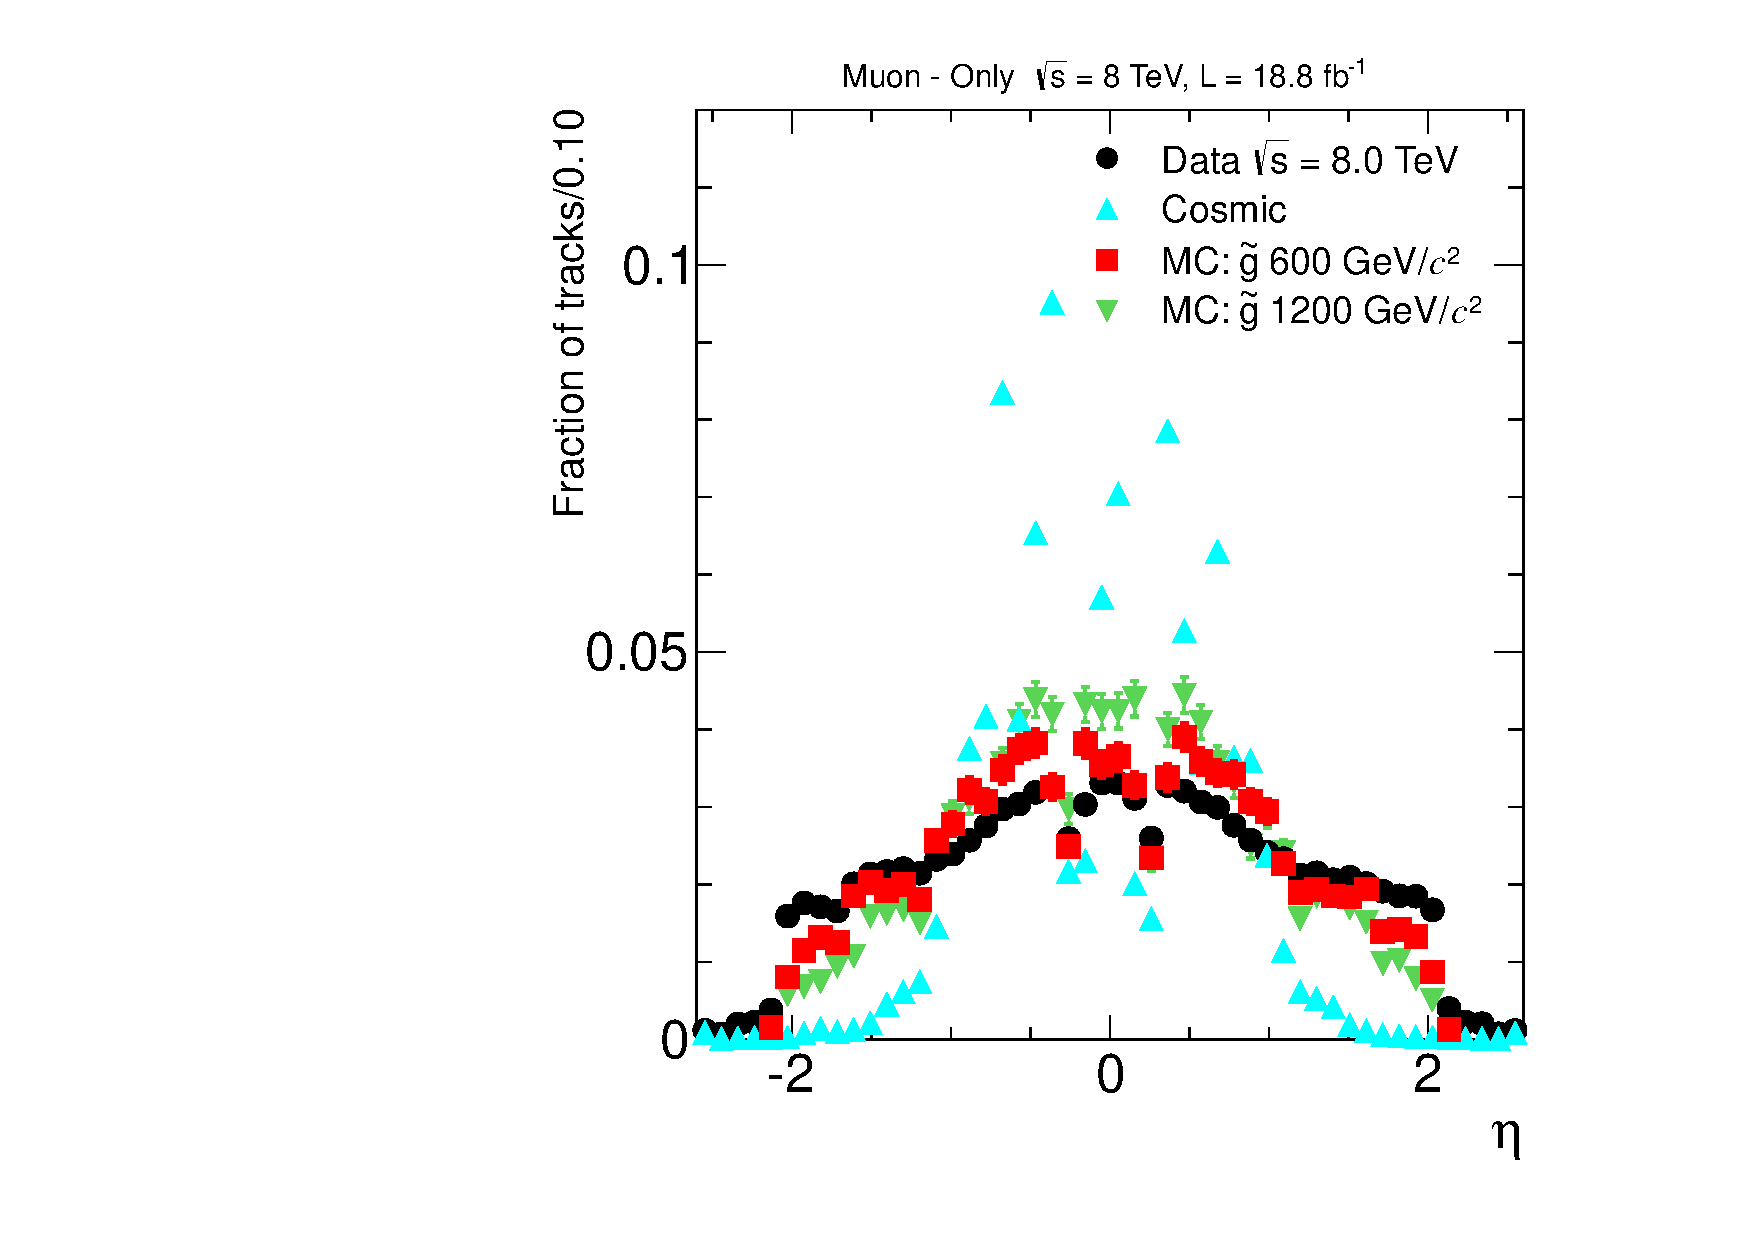
\includegraphics[clip=false, trim=0.0cm 0cm 0.0cm 0cm, width=0.48\textwidth]{figures/muonly/Selection_Comp_8TeV_Cosmic_Eta_BS}
  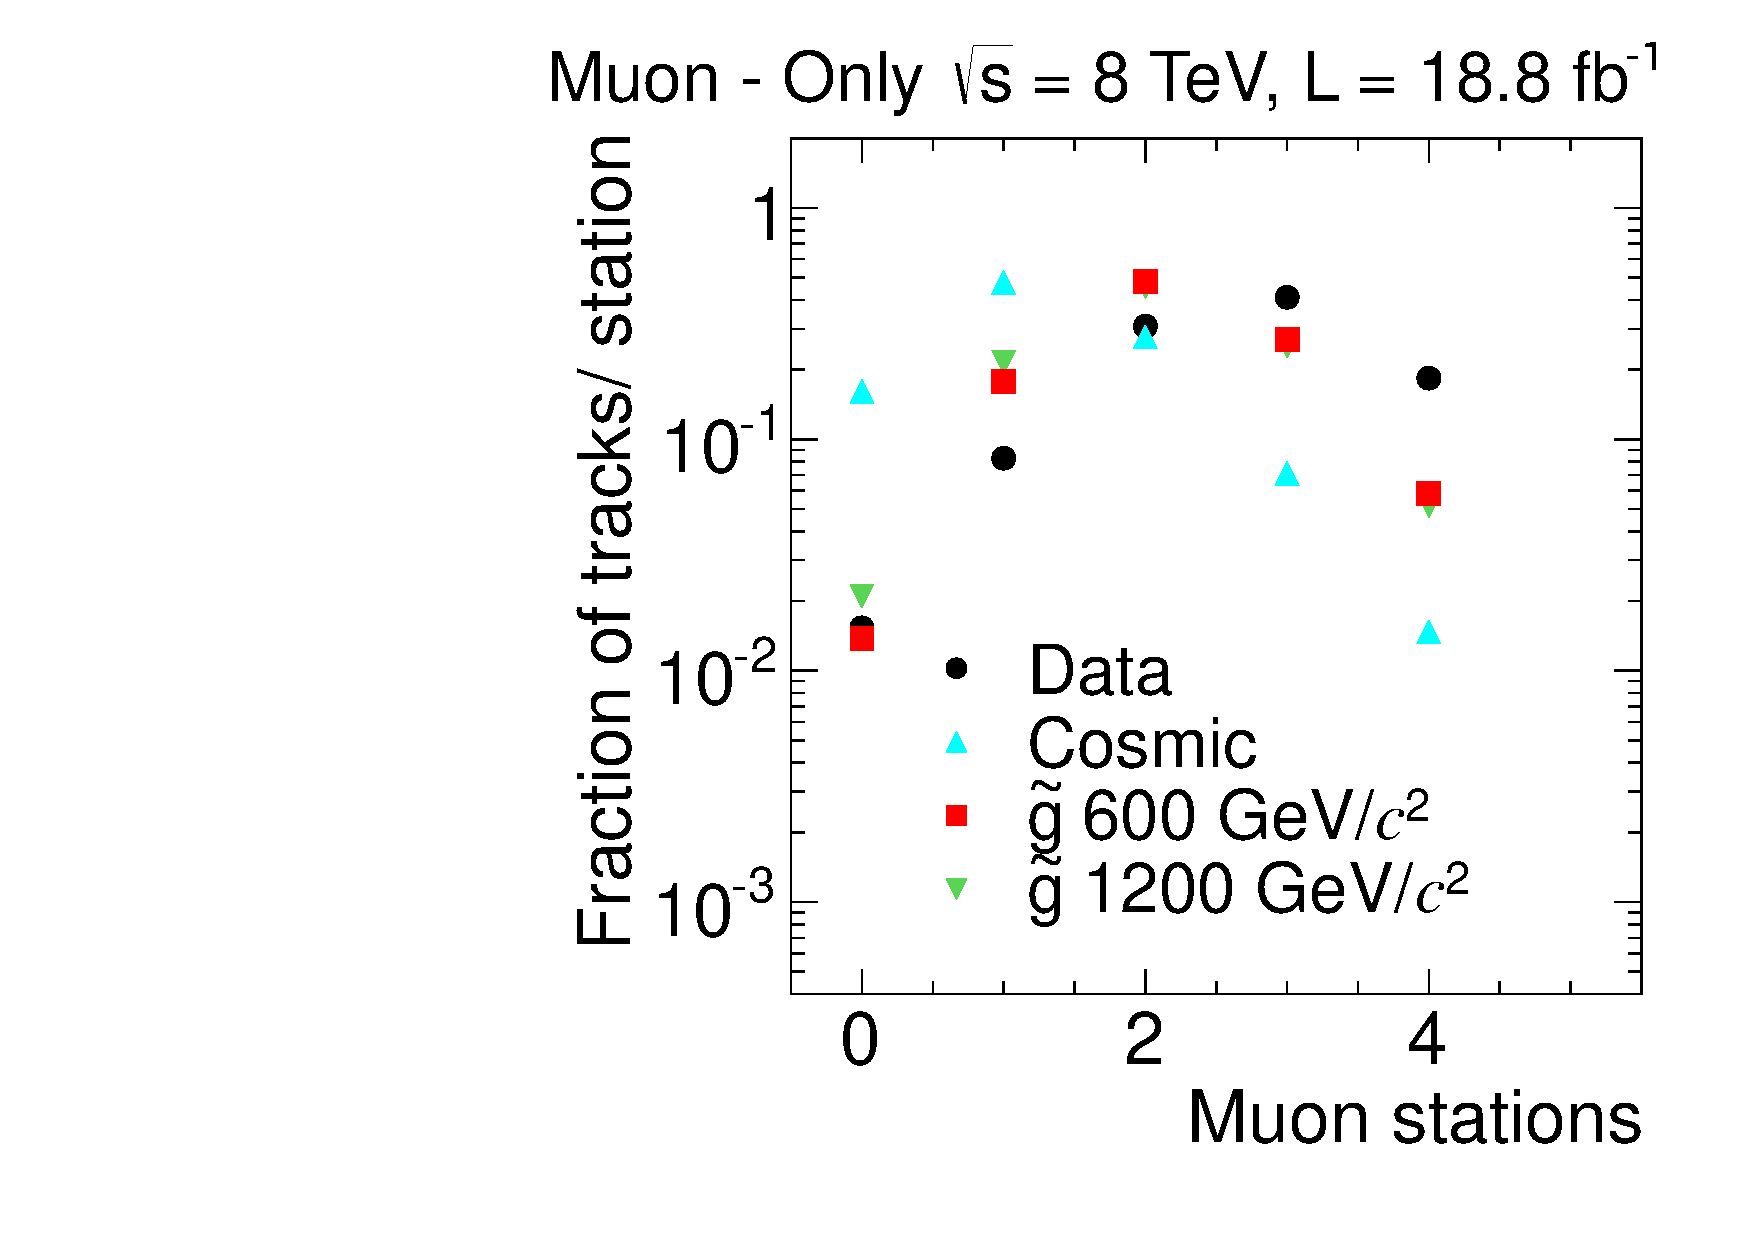
\includegraphics[clip=false, trim=0.0cm 0cm 0.0cm 0cm, width=0.48\textwidth]{figures/muonly/Selection_Comp_8TeV_Cosmic_MatchedStations_BS} \\
\caption[Distribution of $\eta$ and number of matched muon stations for data, cosmic-ray muon control sample, and signal MC samples in the \muononly\ analysis.]
{Distribution of $\eta$ (left) and number of matched muon stations (right) for tracks in the \muononly\ analysis
for data, cosmic-ray muon control sample, and signal MC samples.}
    \label{fig:MuOnlyPreselA}
\end{figure}

\begin{figure}
\centering
  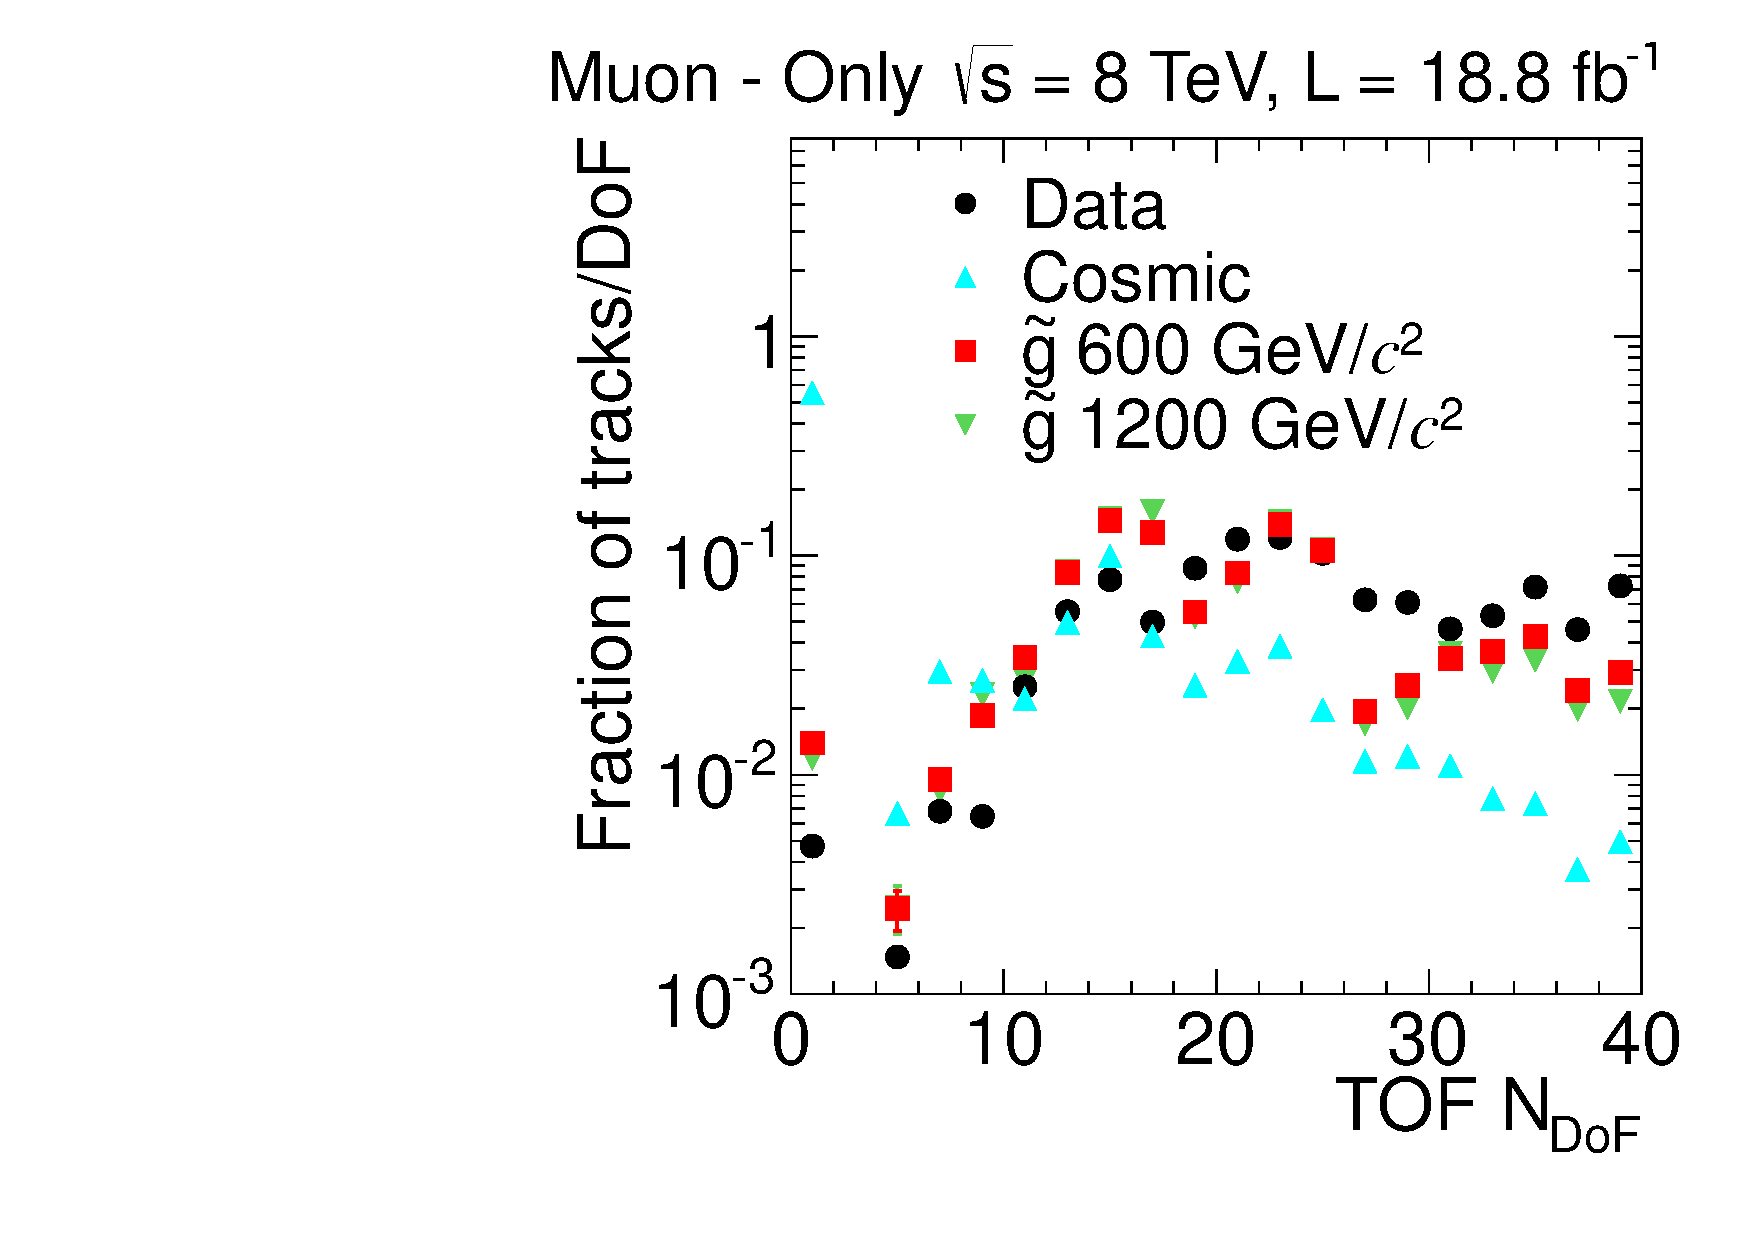
\includegraphics[clip=false, trim=0.0cm 0cm 0.0cm 0cm, width=0.48\textwidth]{figures/muonly/Selection_Comp_8TeV_Cosmic_nDof_BS}
  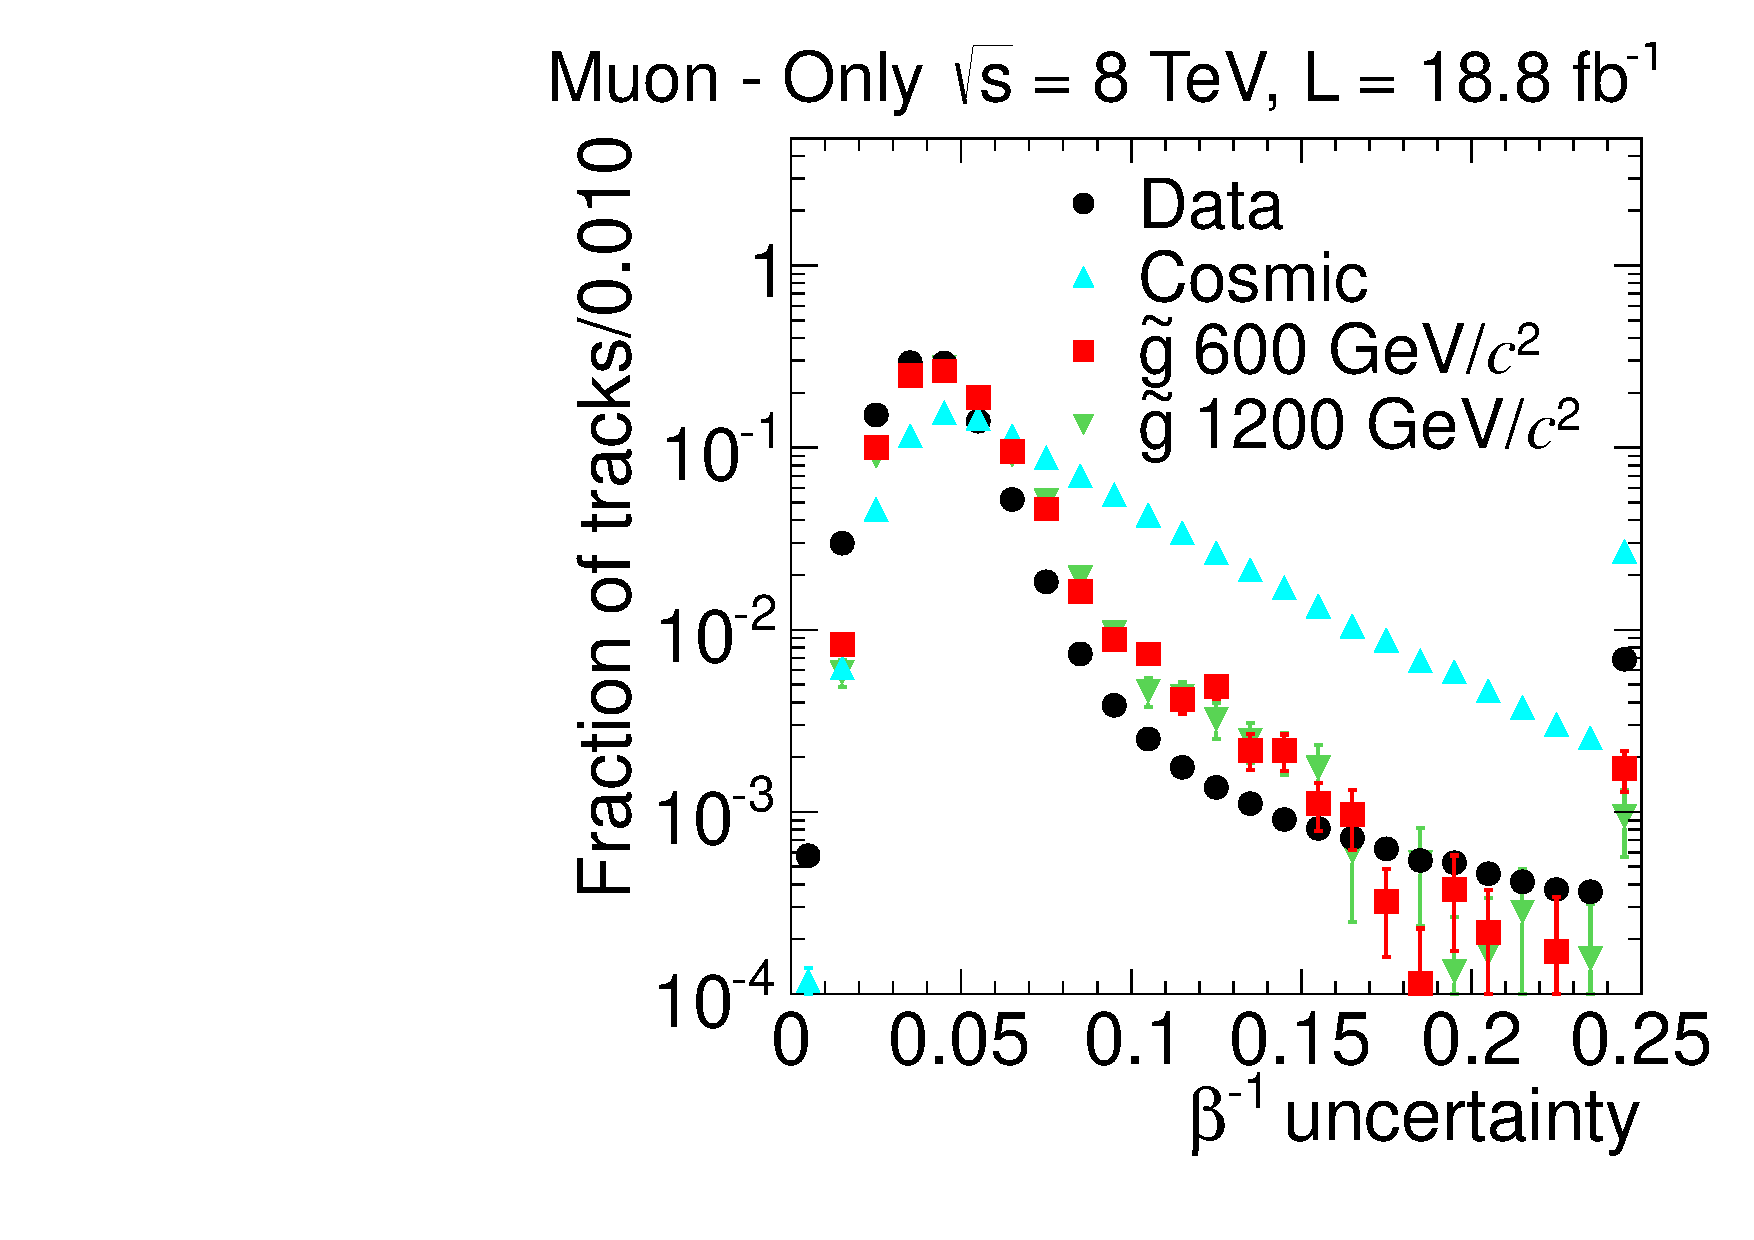
\includegraphics[clip=false, trim=0.0cm 0cm 0.0cm 0cm, width=0.48\textwidth]{figures/muonly/Selection_Comp_8TeV_Cosmic_TOFError_BS} \\
  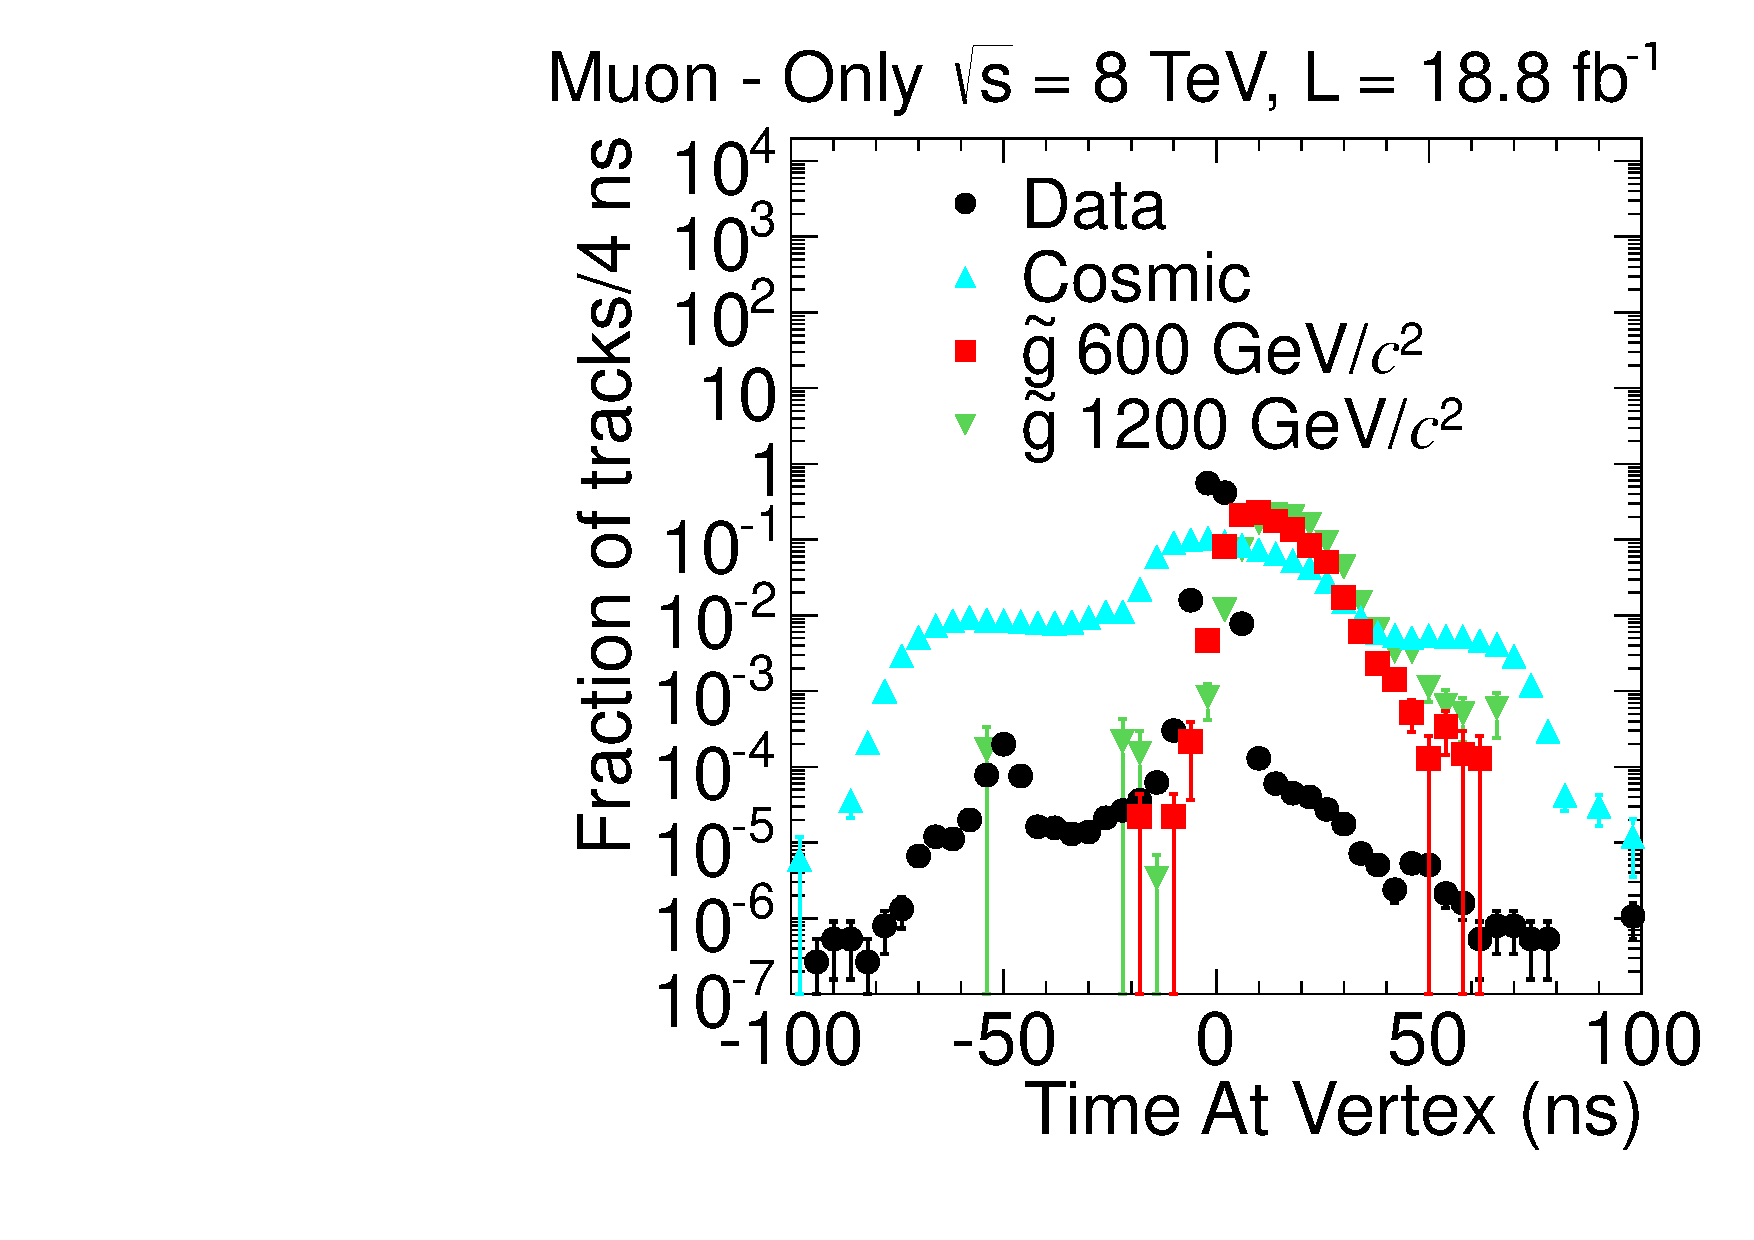
\includegraphics[clip=false, trim=0.0cm 0cm 0.0cm 0cm, width=0.48\textwidth]{figures/muonly/Selection_Comp_8TeV_Cosmic_TimeAtIP_BS} \\
\caption[Distribution of number of degrees of freedom (left) and uncertainty (right) on the \invbeta\ measurement and time at vertex in 
the \muononly\ analysis for data, cosmic-ray muon control sample, and signal MC samples.]
{Distribution of various preselection variables in the \muononly\ analysis for data, cosmic-ray muon control sample, and signal MC samples.
Top row: Number of degrees of freedom (left) and uncertainty (right) on the \invbeta\ measurement.
Bottom row: Time at vertex.}
    \label{fig:MuOnlyPreselB}
\end{figure}

\begin{figure}
\centering
  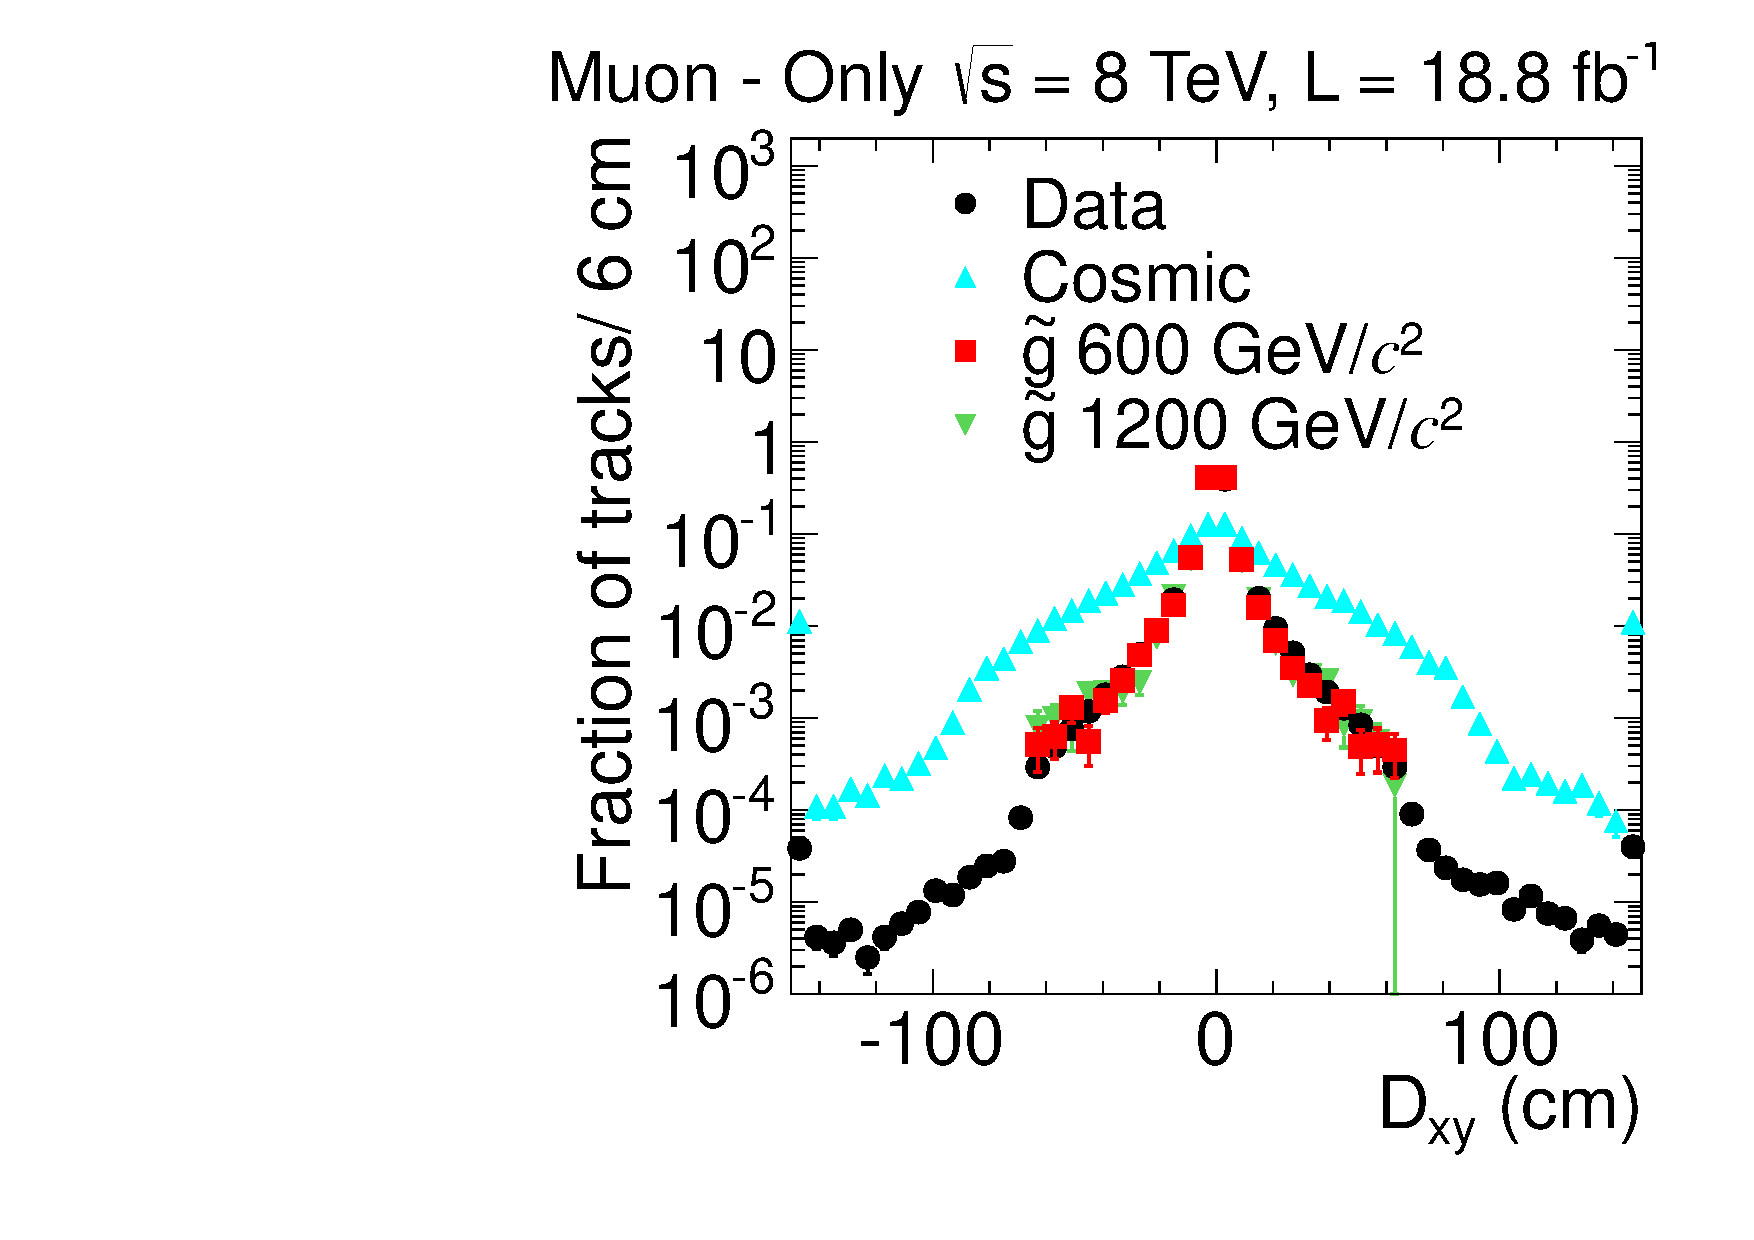
\includegraphics[clip=false, trim=0.0cm 0cm 0.0cm 0cm, width=0.48\textwidth]{figures/muonly/Selection_Comp_8TeV_Cosmic_Dxy_BS}
  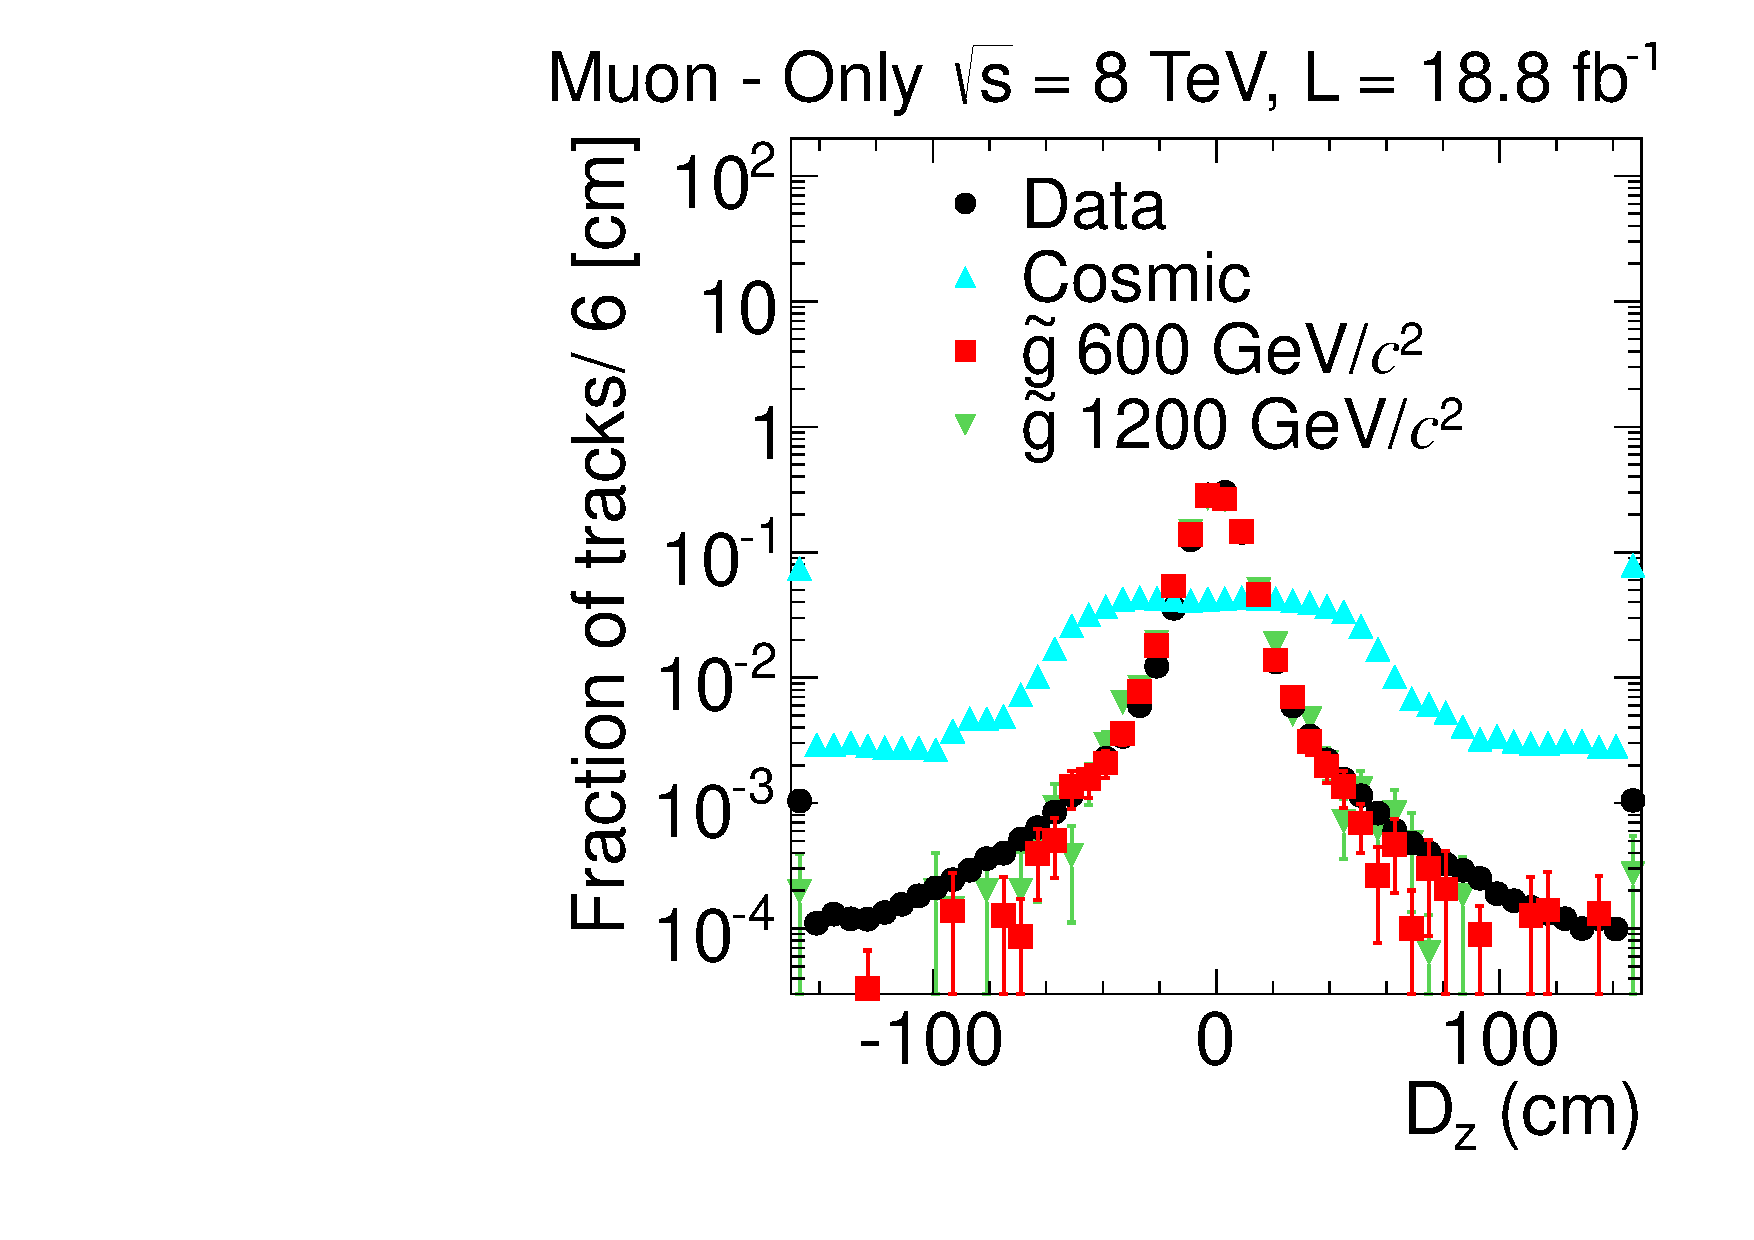
\includegraphics[clip=false, trim=0.0cm 0cm 0.0cm 0cm, width=0.48\textwidth]{figures/muonly/Selection_Comp_8TeV_Cosmic_Dz_BS} \\
  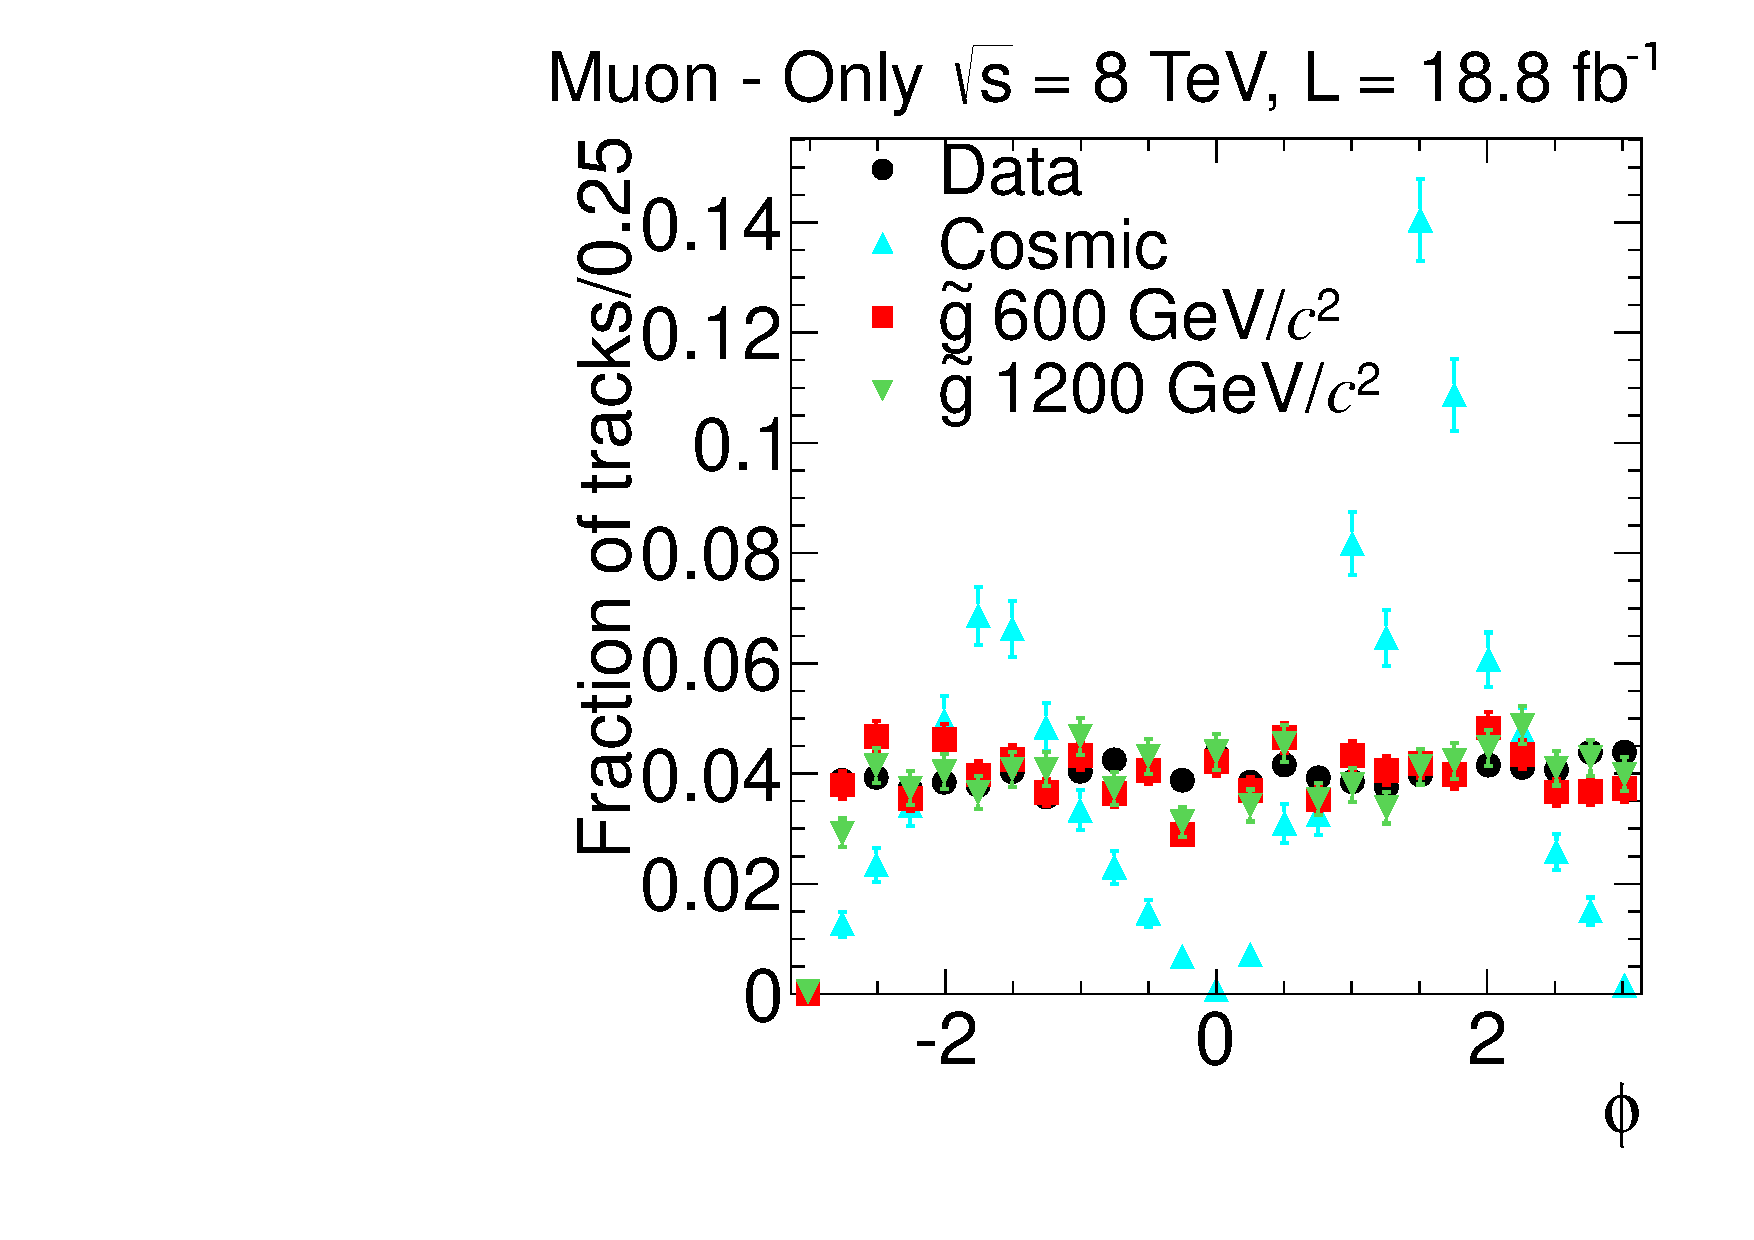
\includegraphics[clip=false, trim=0.0cm 0cm 0.0cm 0cm, width=0.48\textwidth]{figures/muonly/Selection_Comp_8TeV_Cosmic_Phi_BS}
  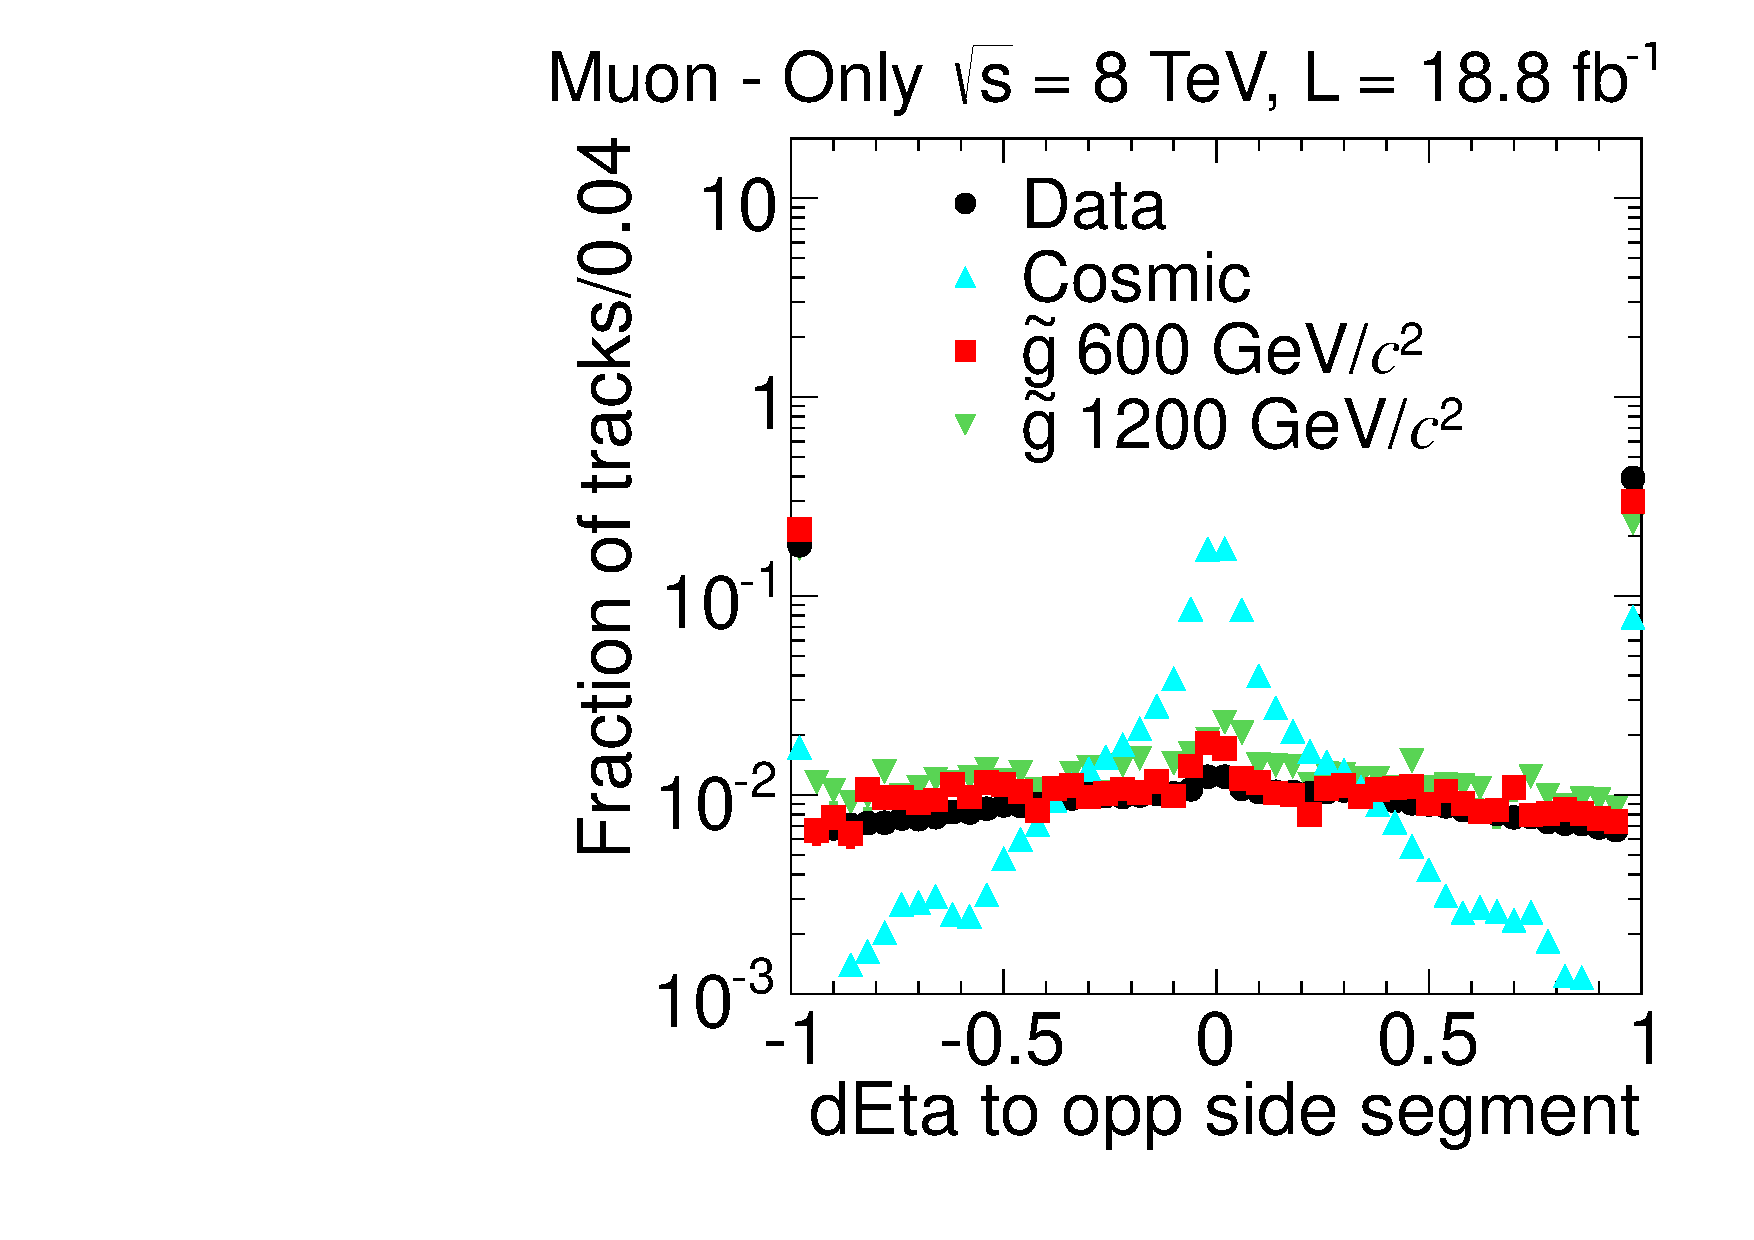
\includegraphics[clip=false, trim=0.0cm 0cm 0.0cm 0cm, width=0.48\textwidth]{figures/muonly/Selection_Comp_8TeV_Cosmic_SegMinEtaSep_BS}
  \caption[Distribution of transverse and longitudinal displacement, $\phi$, and $\eta$ separation to muon segments
in the \muononly\ analysis for data, cosmic-ray muon control sample, and signal MC samples.]
{Distribution of various preselection variables in the \muononly\ analysis for data, cosmic-ray muon control sample, and signal MC samples.
Top row: Distribution of transverse (left) and longitudinal displacement (right).
Bottom row: Distribution of the $\phi$ of the track (left) and the $\eta$ separation of the track to muon segments (right). The rightmost bin in the
$\eta$ separation plot includes tracks where no segments were found.}
    \label{fig:MuOnlyPreselC}
\end{figure}

\subsection{Preselection for \tktof\ \label{sec:tktofpreselection}}

The \tktof\ analysis applies cuts on the inner tracker track, which has a much better $p_T$ and impact parameter resolution than the muon system track.
The track is required to have $p_T > 45$~GeV and  $|\eta| < 2.1$ to match the trigger level requirements. 
Quality cuts are applied as low quality background tracks can have mismeasured momentum and potentially high fluctuations in \dedx.
The inner track is required to have at least eight hits in the inner tracker with at least two coming from the pixel detector. At least 80\% of the hits associated with the track
must be considered valid. As in~\cite{Chatrchyan:2012sp}, a cleaning procedure is applied to the hits before calculating \dedx\ that is 
intended to remove anomalous energy loss from overlapping tracks, nuclear interactions, and hard $\delta$-rays.
There must be at least six measurements passing this cleaning.
Figure~\ref{fig:TkMuPreselA} shows these variables for data and signal MC samples.

\begin{figure}
\centering
  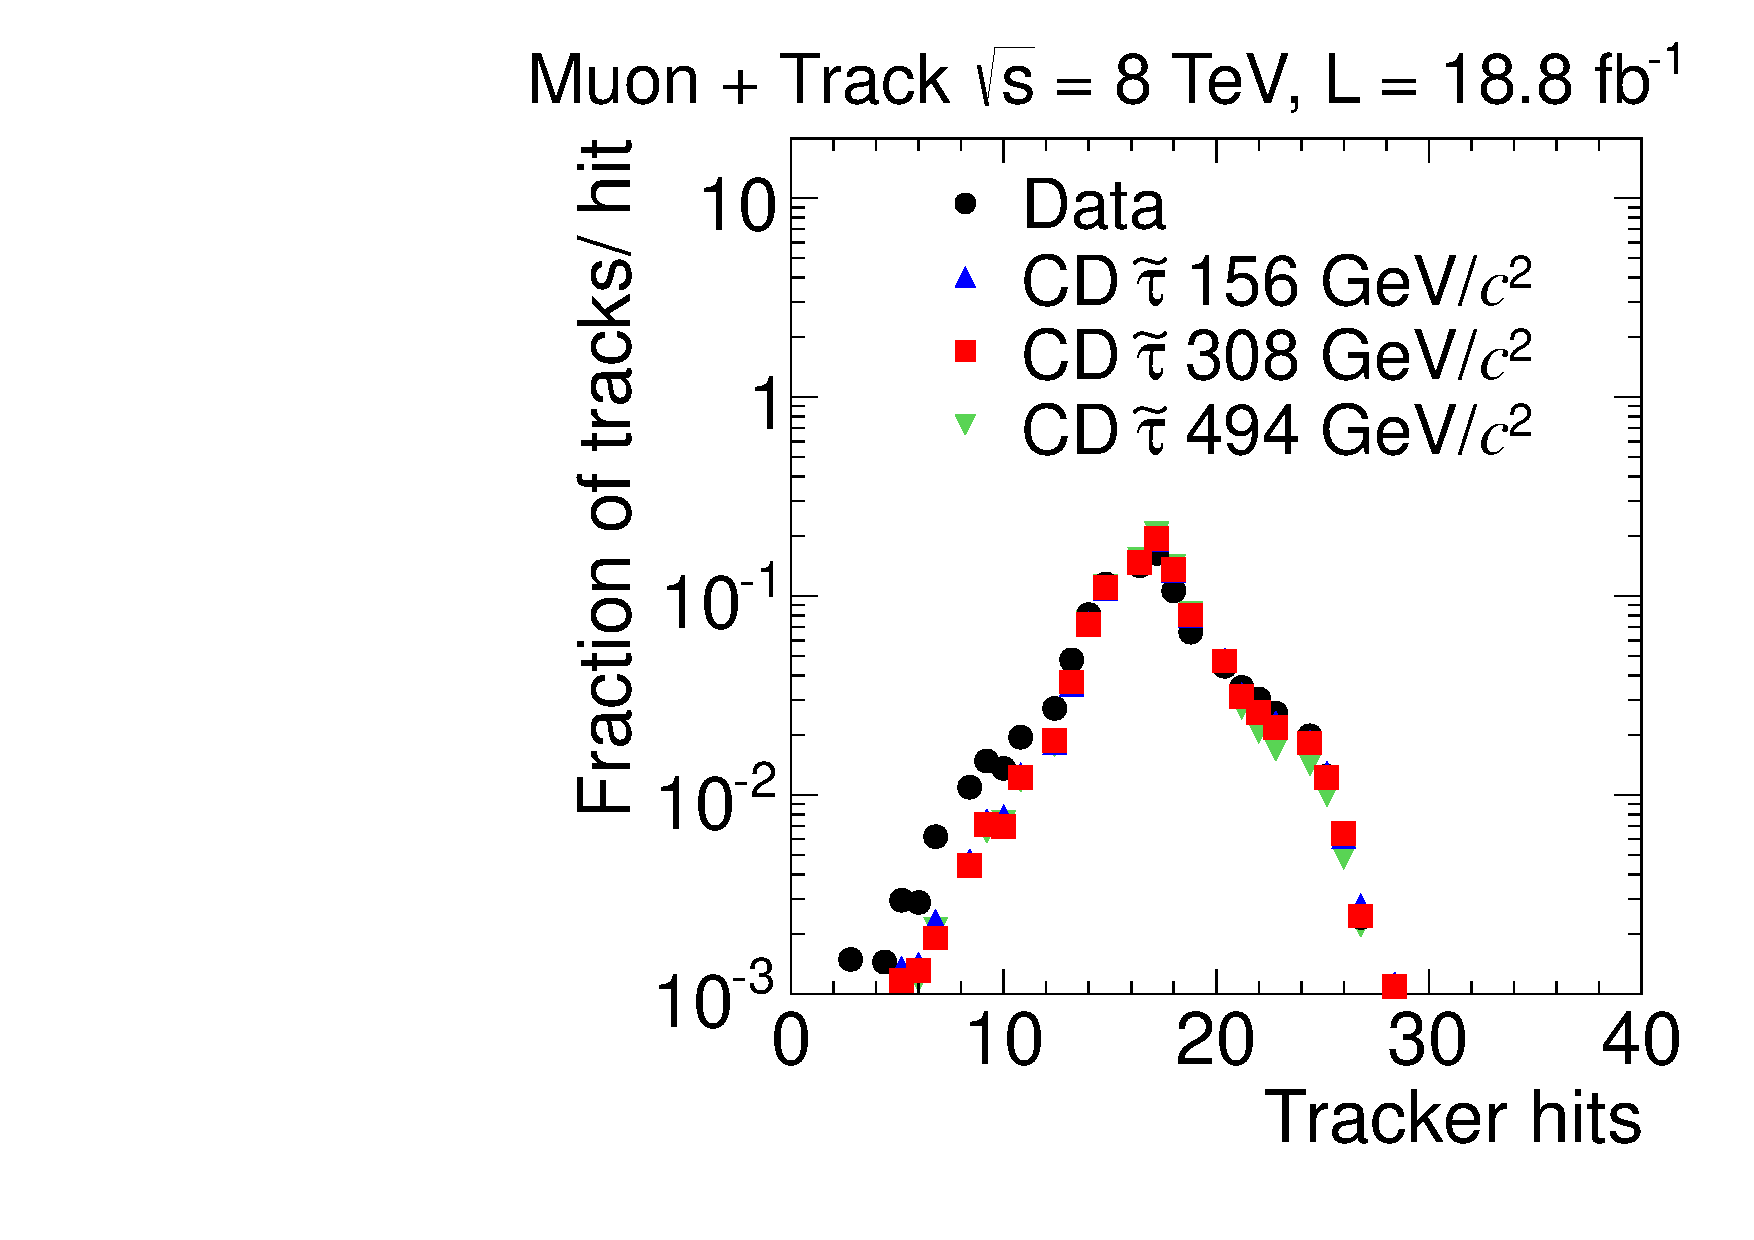
\includegraphics[clip=false, trim=0.0cm 0cm 0.0cm 0cm, width=0.48\textwidth]{figures/tkmu/Selection_Comp_8TeV_GMStau_NOH_BS}
  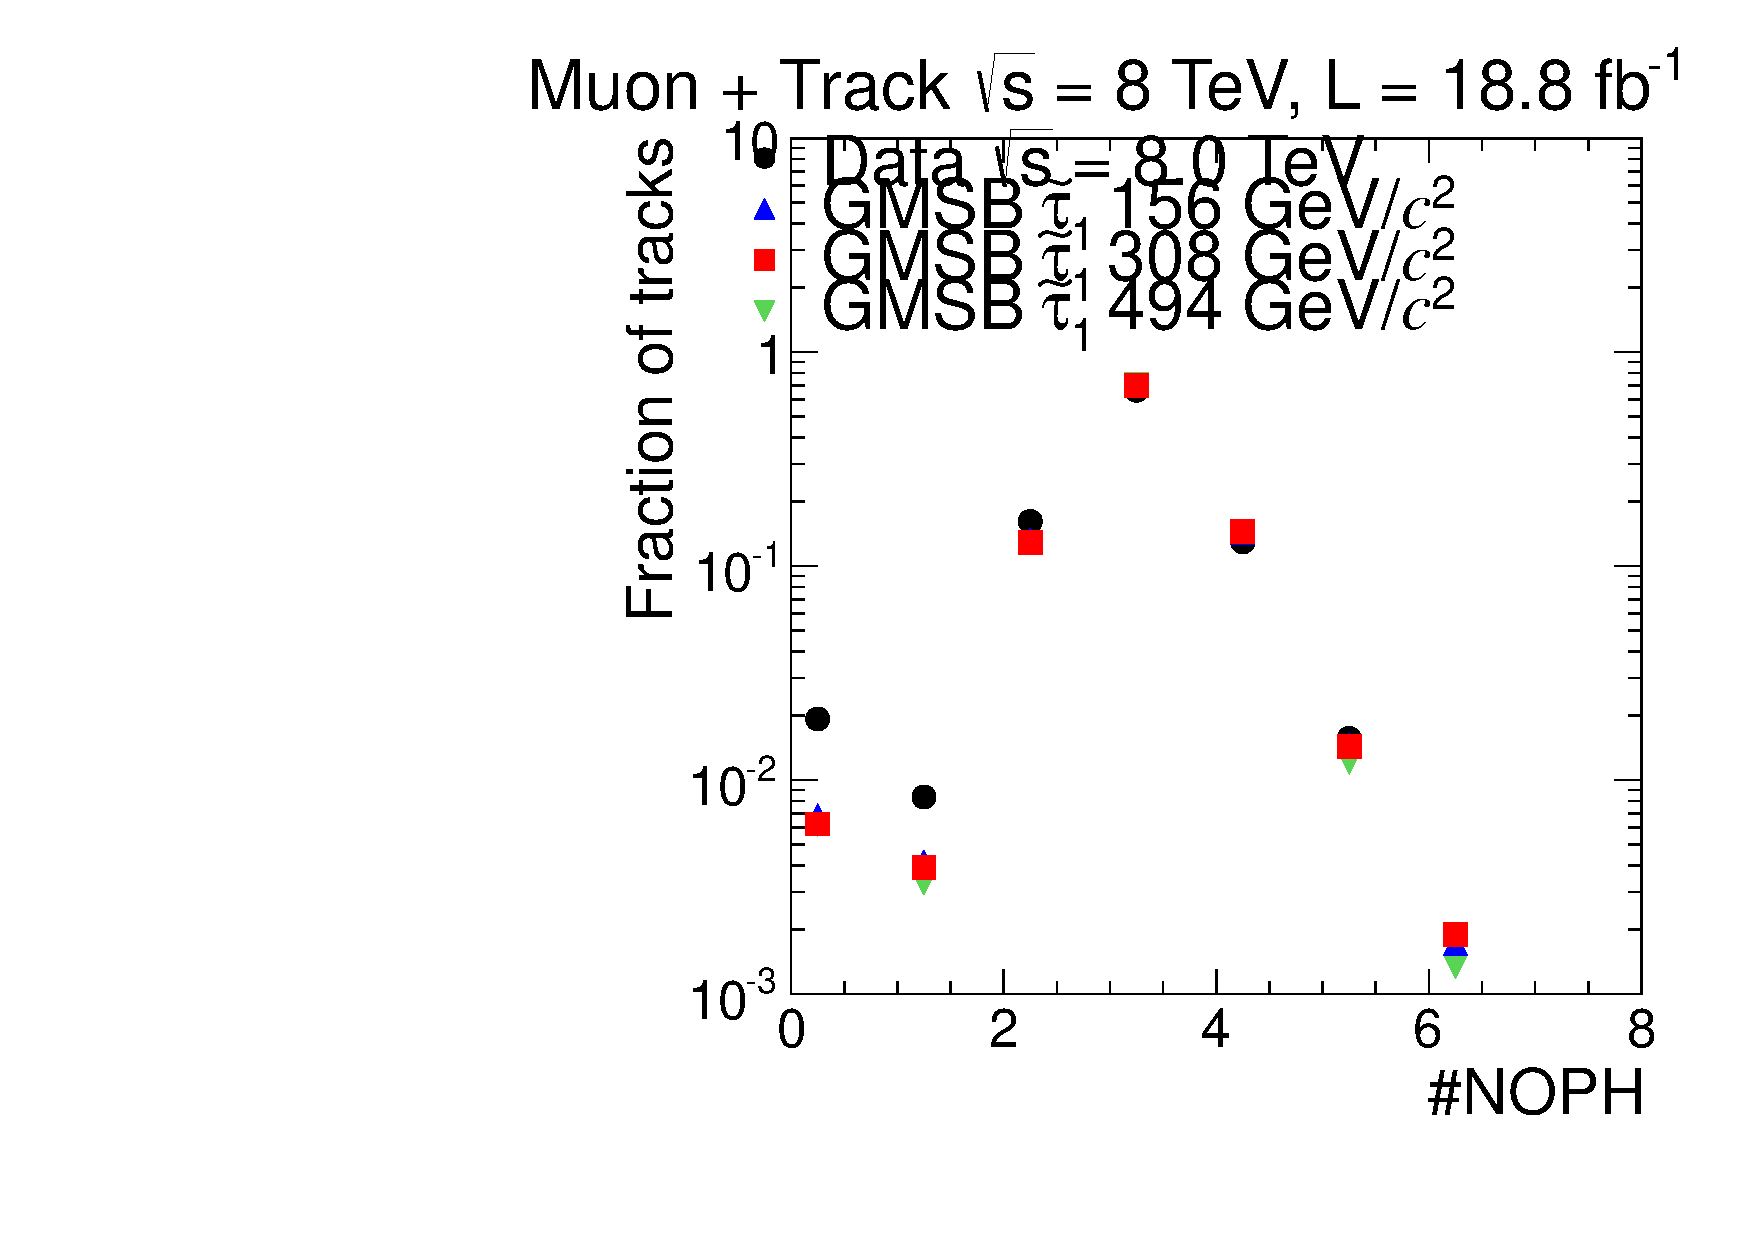
\includegraphics[clip=false, trim=0.0cm 0cm 0.0cm 0cm, width=0.48\textwidth]{figures/tkmu/Selection_Comp_8TeV_GMStau_NOPH_BS} \\
  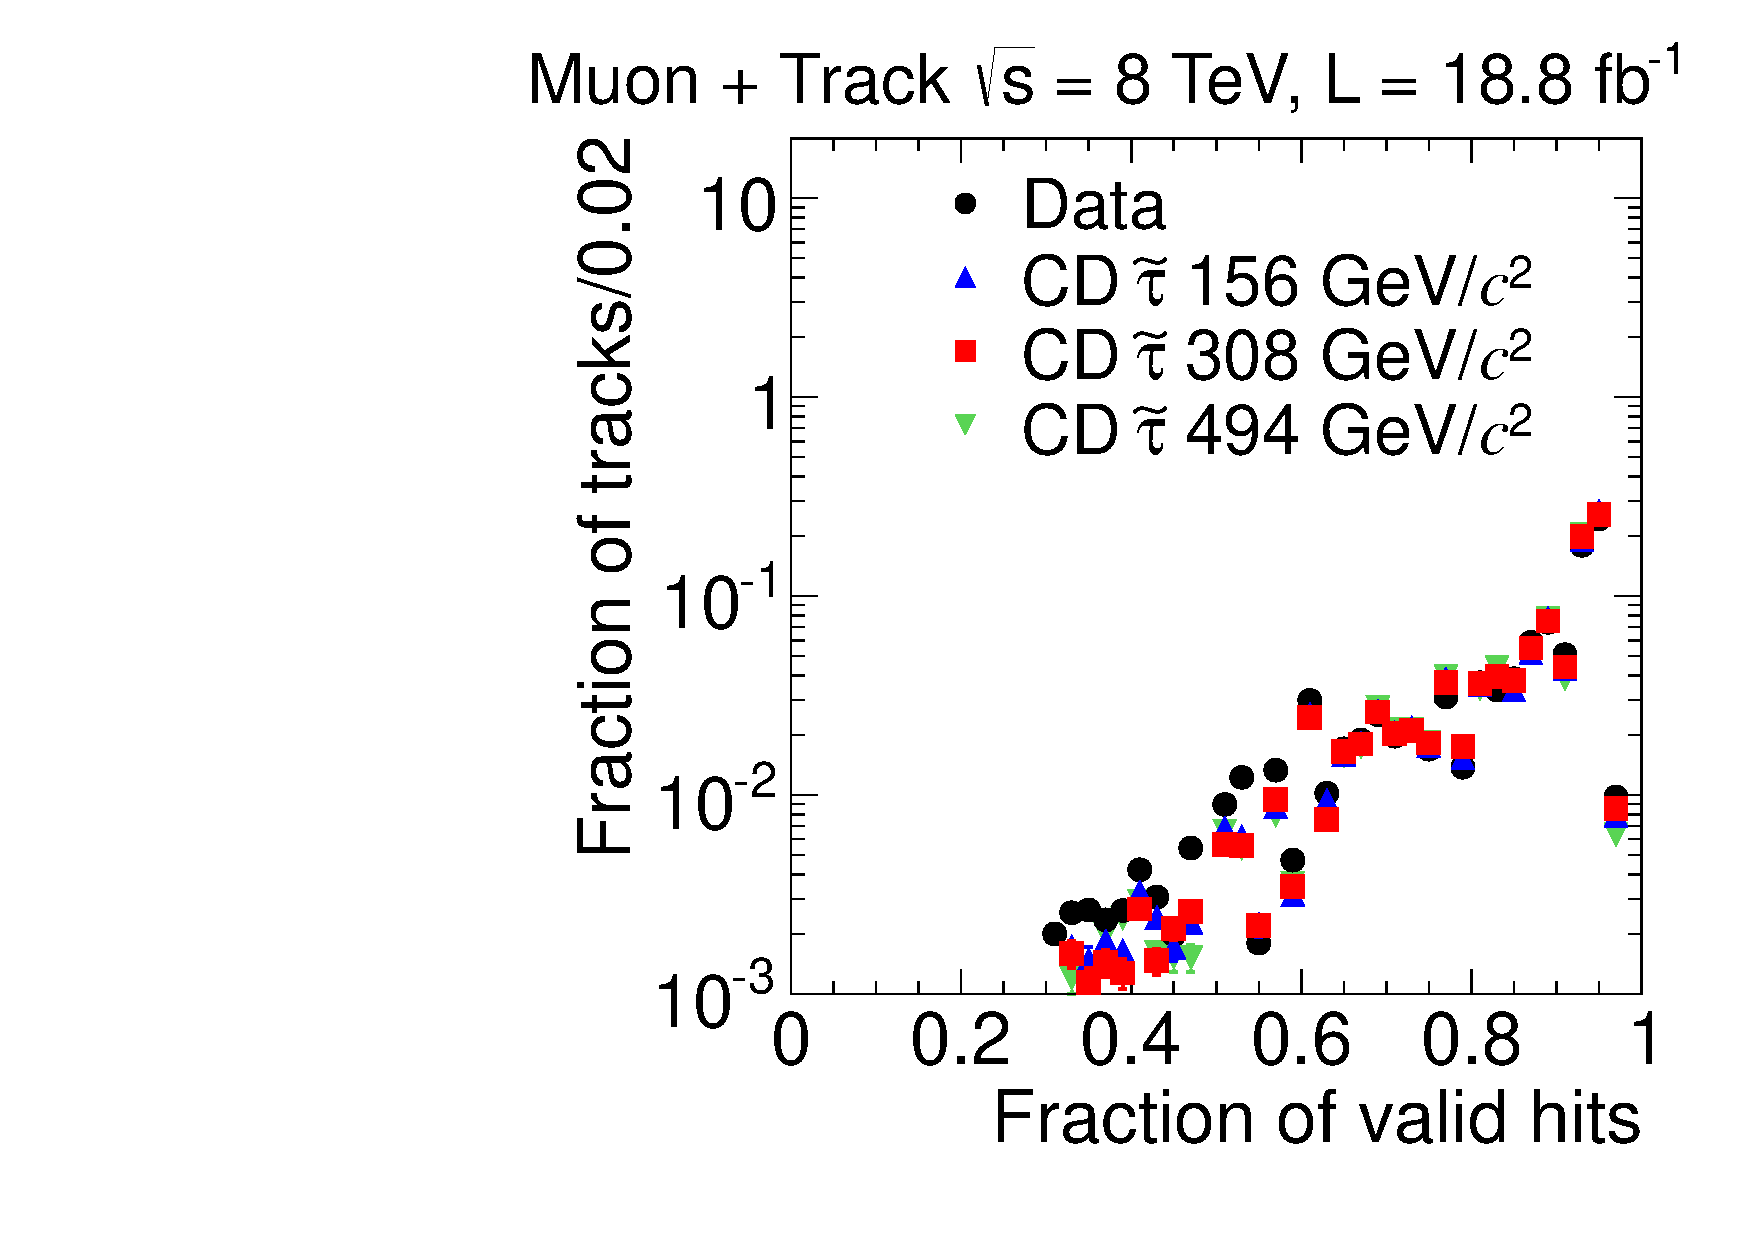
\includegraphics[clip=false, trim=0.0cm 0cm 0.0cm 0cm, width=0.48\textwidth]{figures/tkmu/Selection_Comp_8TeV_GMStau_NOHFraction_BS}
  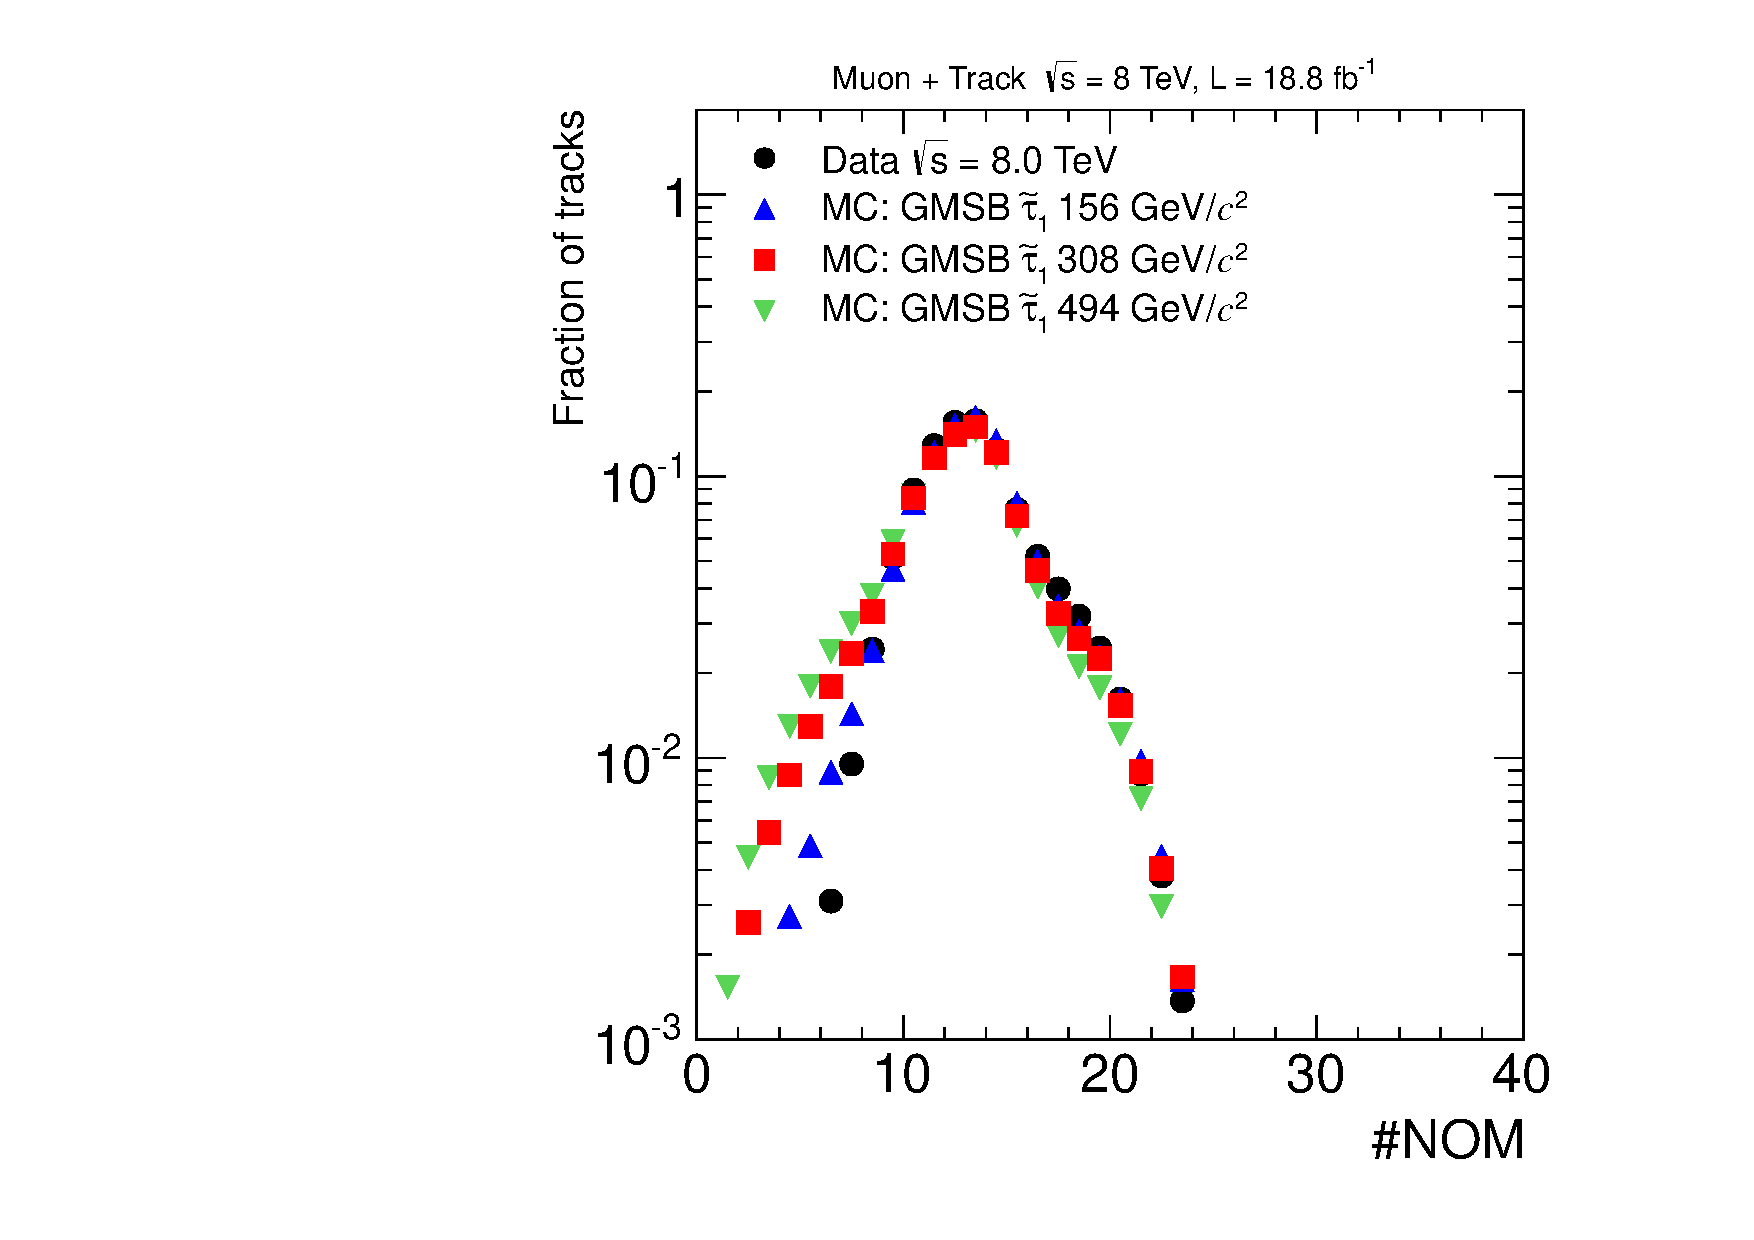
\includegraphics[clip=false, trim=0.0cm 0cm 0.0cm 0cm, width=0.48\textwidth]{figures/tkmu/Selection_Comp_8TeV_GMStau_NOM_BS}
  \caption[Distribution of number of tracker and pixel hits, fraction of valid tracker hits, and number of \dedx\ measurements in the \tktof\ analysis for data and signal MC samples.]
{Distribution of various preselection variables in the \tktof\ analysis for data and signal MC samples.
Top row: Number of tracker (left) and pixel (right) hits.
Bottom row: Fraction of valid tracker hits (left) and number of measurements used for the \dedx\ calculation (right).}
    \label{fig:TkMuPreselA}
\end{figure}

The relative uncertainty on the track $p_T$ ($\sigma_{p_T}/p_T$) must be less than 0.25 and the $\chi^2$ per degree of freedom must be less than five.
While cosmic-ray muons are expected to be a negligible background in the \tktof\ analysis, loose cuts are placed on the impact parameter of the track;
these cuts are nearly 100\% efficient for signal particles.
The displacement of the track with respect to the primary vertex
with the smallest longitudinal displacement must be less than 0.5~cm in both the transverse and longitudinal directions.
Figure~\ref{fig:TkMuPreselB} shows the $p_T$ uncertainty, $\chi^2$ per degree of freedom, and $d_z$ and $d_{xy}$ displacement for data and signal MC samples.

\begin{figure}
\centering
  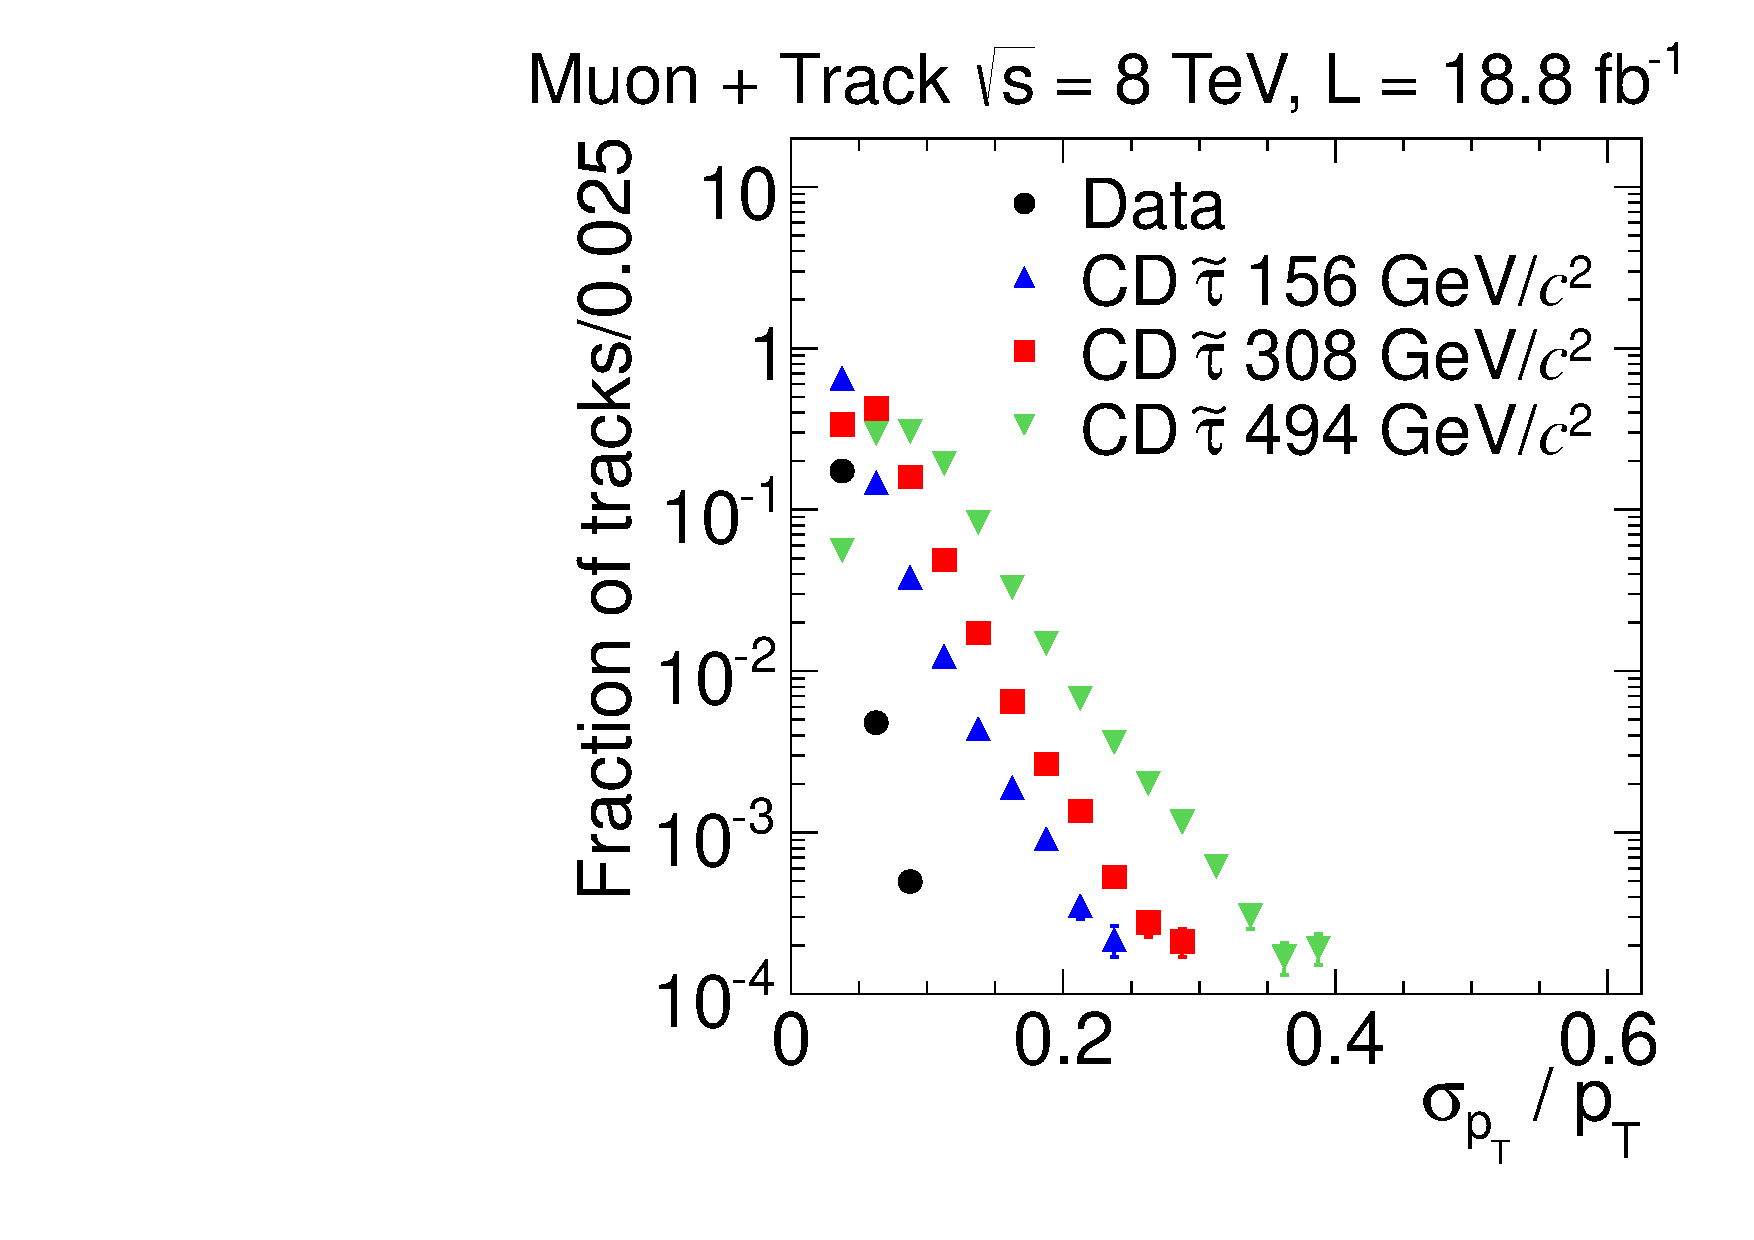
\includegraphics[clip=false, trim=0.0cm 0cm 0.0cm 0cm, width=0.48\textwidth]{figures/tkmu/Selection_Comp_8TeV_GMStau_Pterr_BS}
  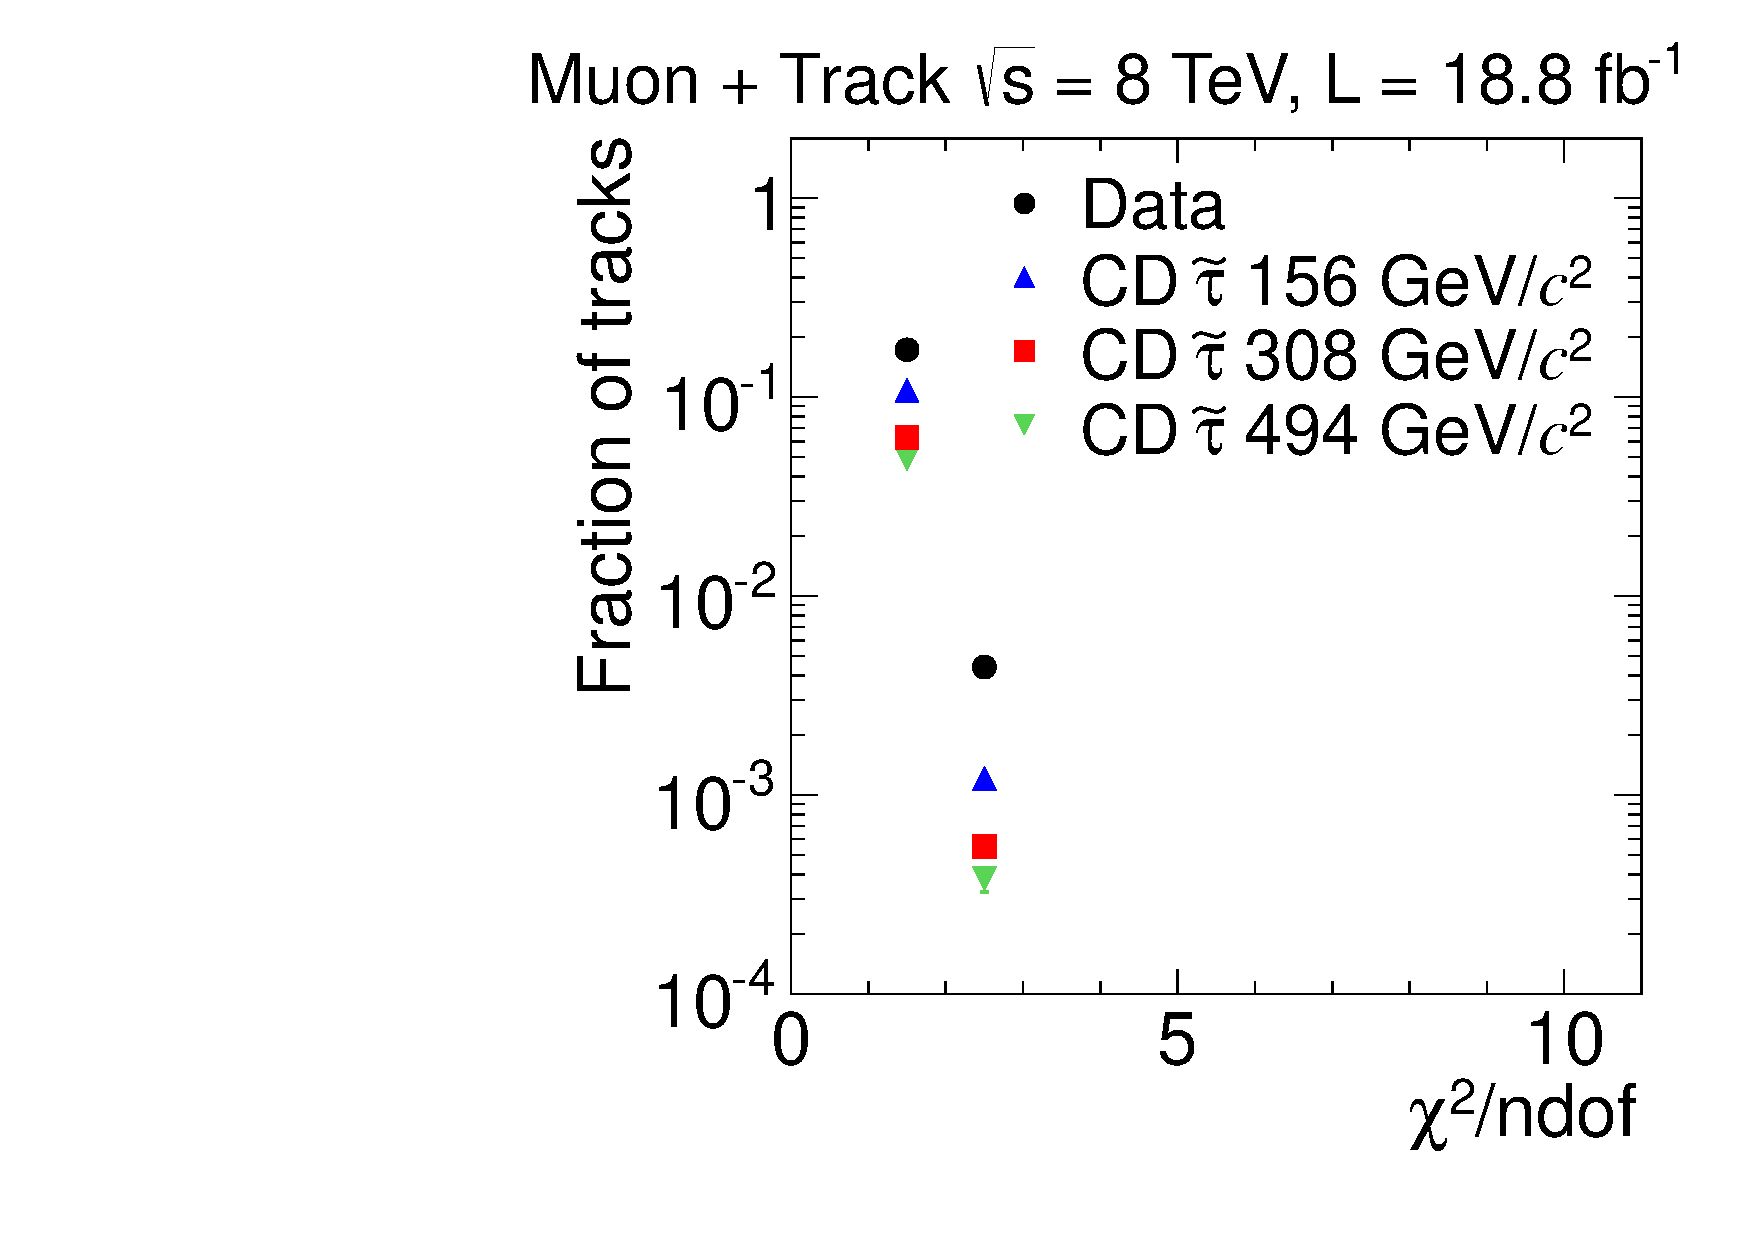
\includegraphics[clip=false, trim=0.0cm 0cm 0.0cm 0cm, width=0.48\textwidth]{figures/tkmu/Selection_Comp_8TeV_GMStau_Chi2_BS} \\
  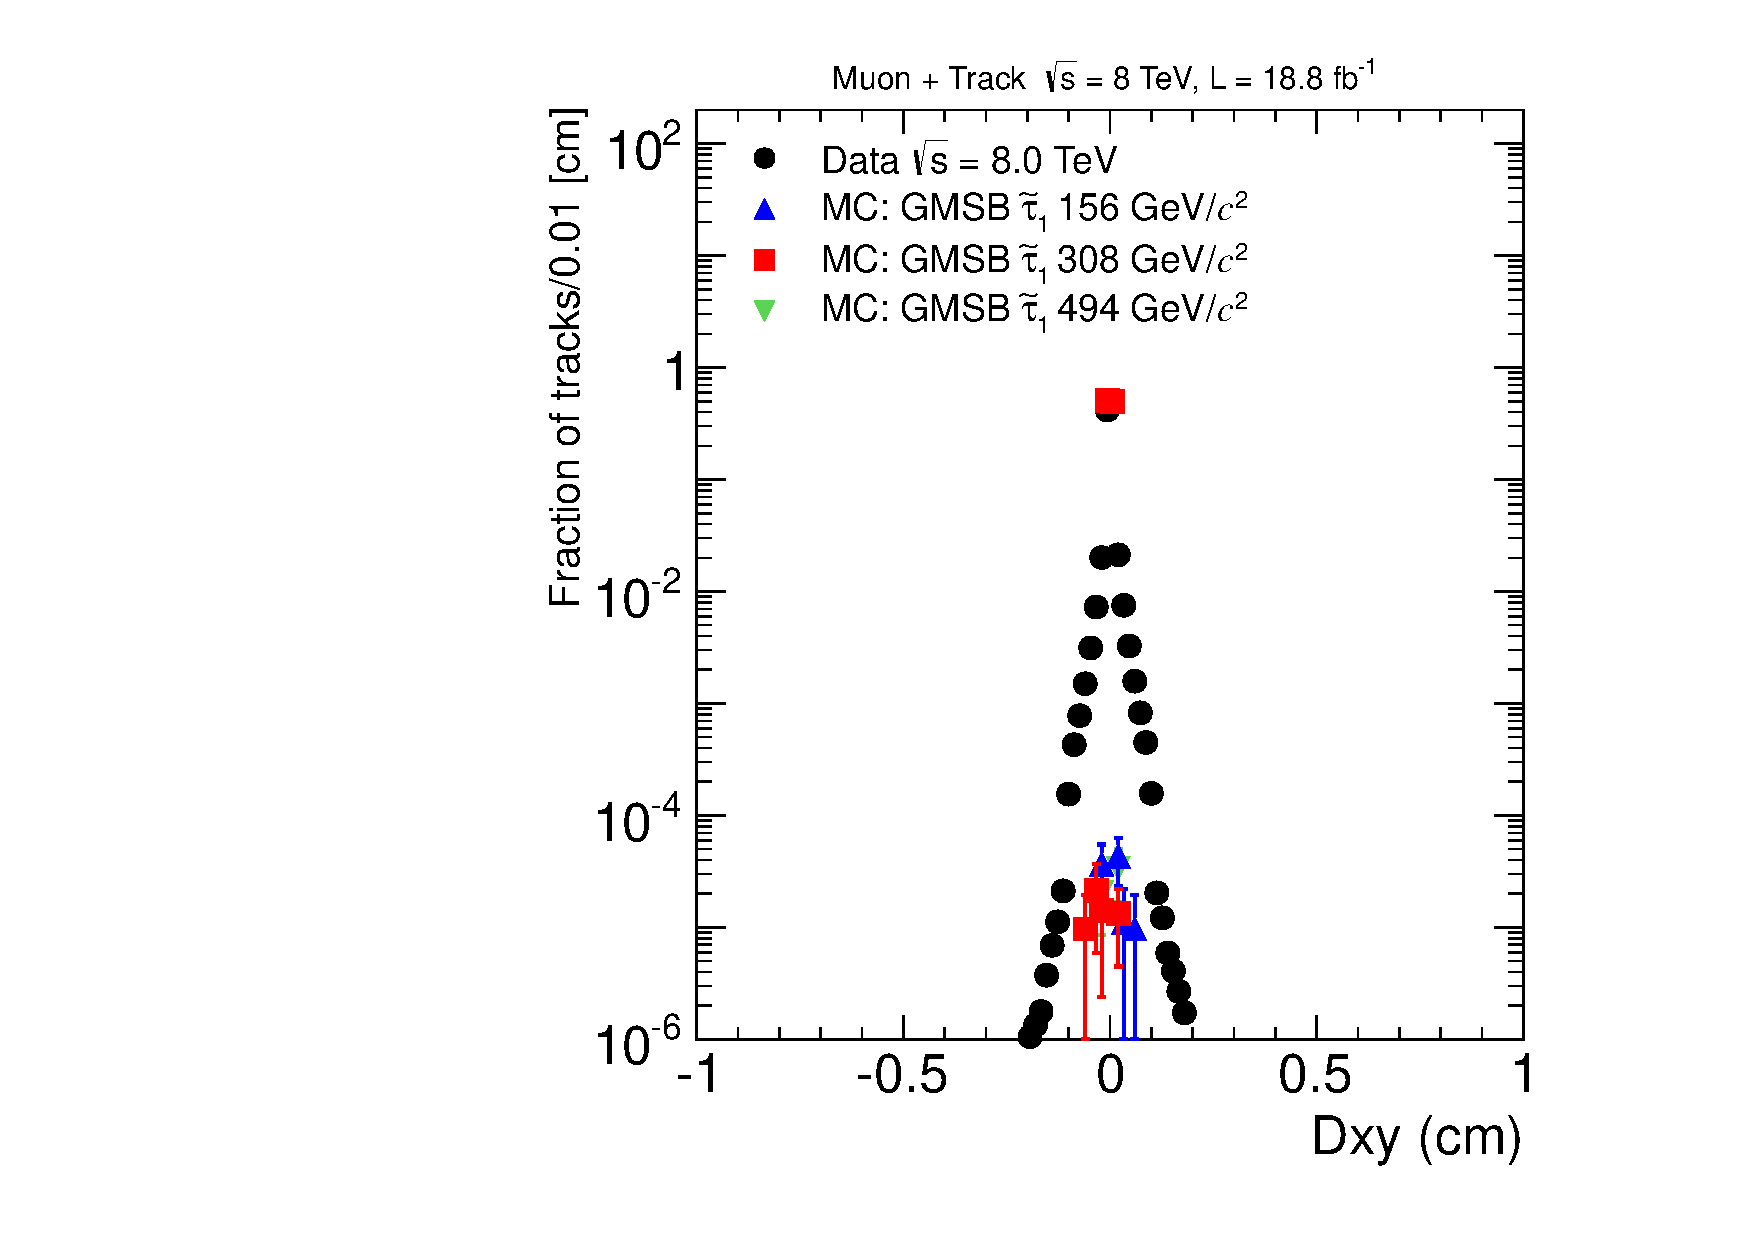
\includegraphics[clip=false, trim=0.0cm 0cm 0.0cm 0cm, width=0.48\textwidth]{figures/tkmu/Selection_Comp_8TeV_GMStau_Dxy_BS}
  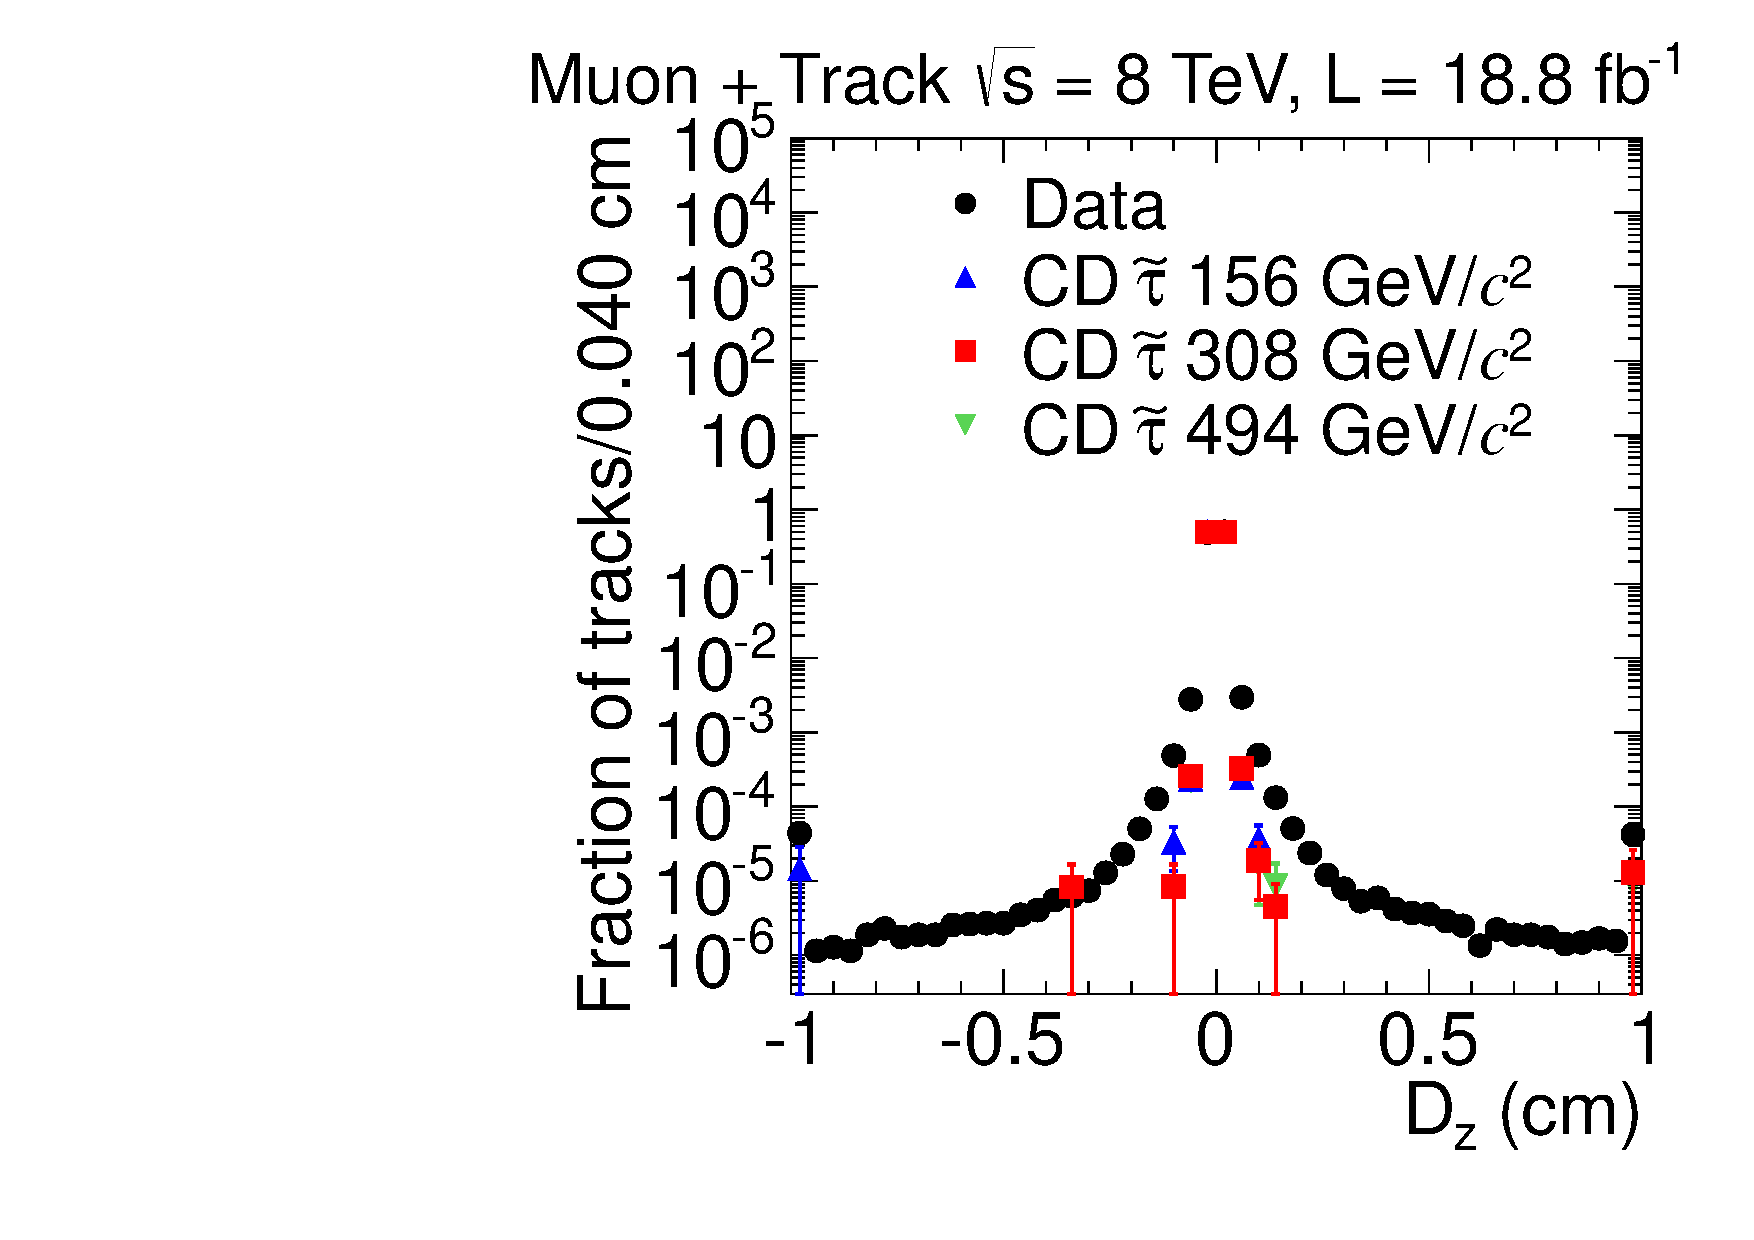
\includegraphics[clip=false, trim=0.0cm 0cm 0.0cm 0cm, width=0.48\textwidth]{figures/tkmu/Selection_Comp_8TeV_GMStau_Dz_BS}
  \caption[Distribution of relative \pt\ uncertainty, $\chi^2$ per degree of freedom, and transverse and longitudinal
displacement in the \tktof\ analysis for data and signal MC samples.]
{Distribution of various preselection variables in the \tktof\ analysis for data and signal MC samples.
Top row: Relative $p_T$ uncertainty (left) and $\chi^2$ per degree of freedom (right).
Bottom row: Displacement in the transverse (left) and longitudinal (right) directions.}
    \label{fig:TkMuPreselB}
\end{figure}

Isolation cuts are also applied in the \tktof\ analysis. Isolated means that there not be high energy particles near the track.
This is required to reduce the background from jets where overlapping tracks could give
anomalously high \dedx\ values. The isolation cuts are kept very loose as the goal is not to find isolated particles but just to reject very high energy jets.
Specifically, the sum of the momentum of the tracks within 0.3 in $\eta-\phi$ 
space of the track (excluding the track itself) is required to be less than 50 GeV. Additionally, the total
amount of energy measured in the calorimeter within a radius of 0.3 in $\eta-\phi$ space to the track divided by the track momentum must be less than 0.3.

Additionally, the \tktof\ analysis uses the same cuts on the \invbeta\ uncertainty and number of measurements as the \muononly\ analysis.
Figure~\ref{fig:TkMuPreselC} shows the isolation and \invbeta\ variables for data and signal MC samples.

\begin{figure}
\centering
  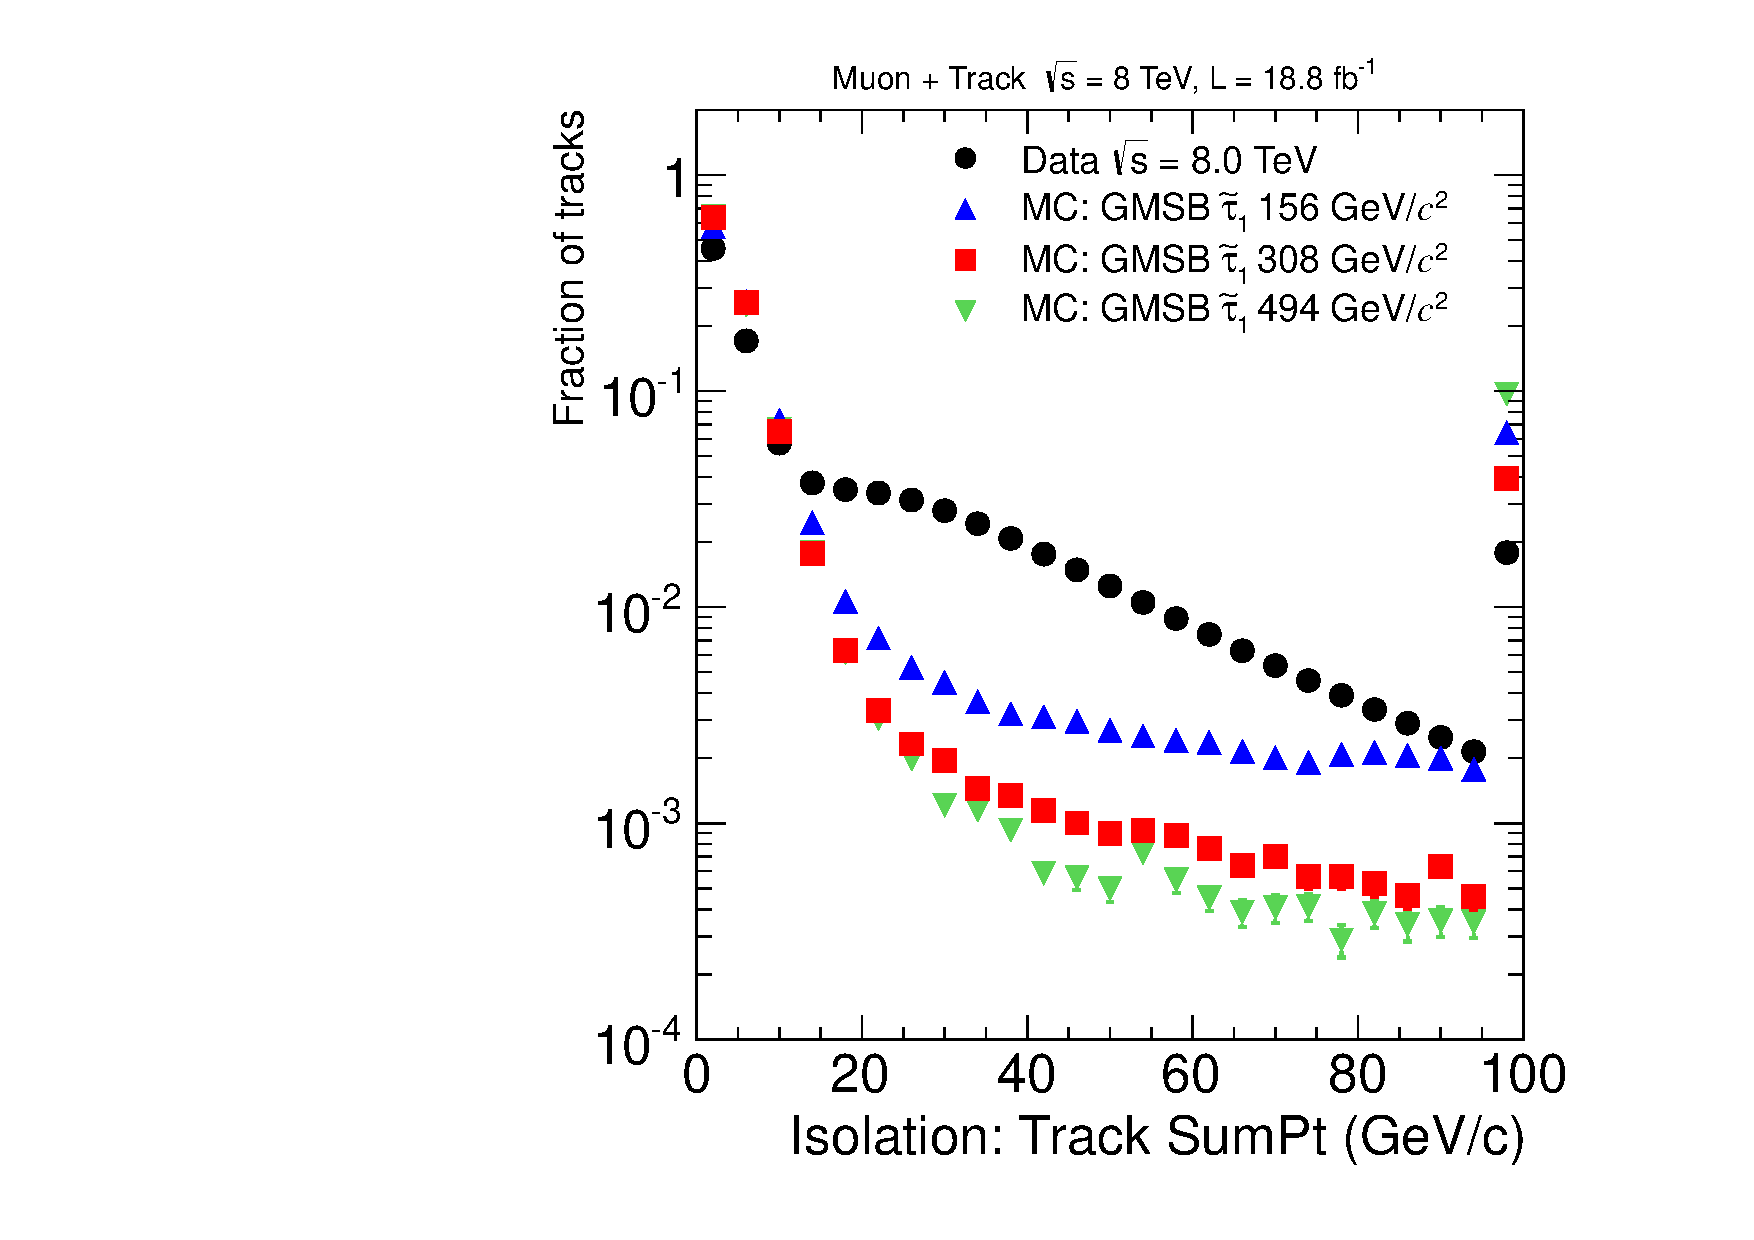
\includegraphics[clip=false, trim=0.0cm 0cm 0.0cm 0cm, width=0.48\textwidth]{figures/tkmu/Selection_Comp_8TeV_GMStau_IsolT_BS}
  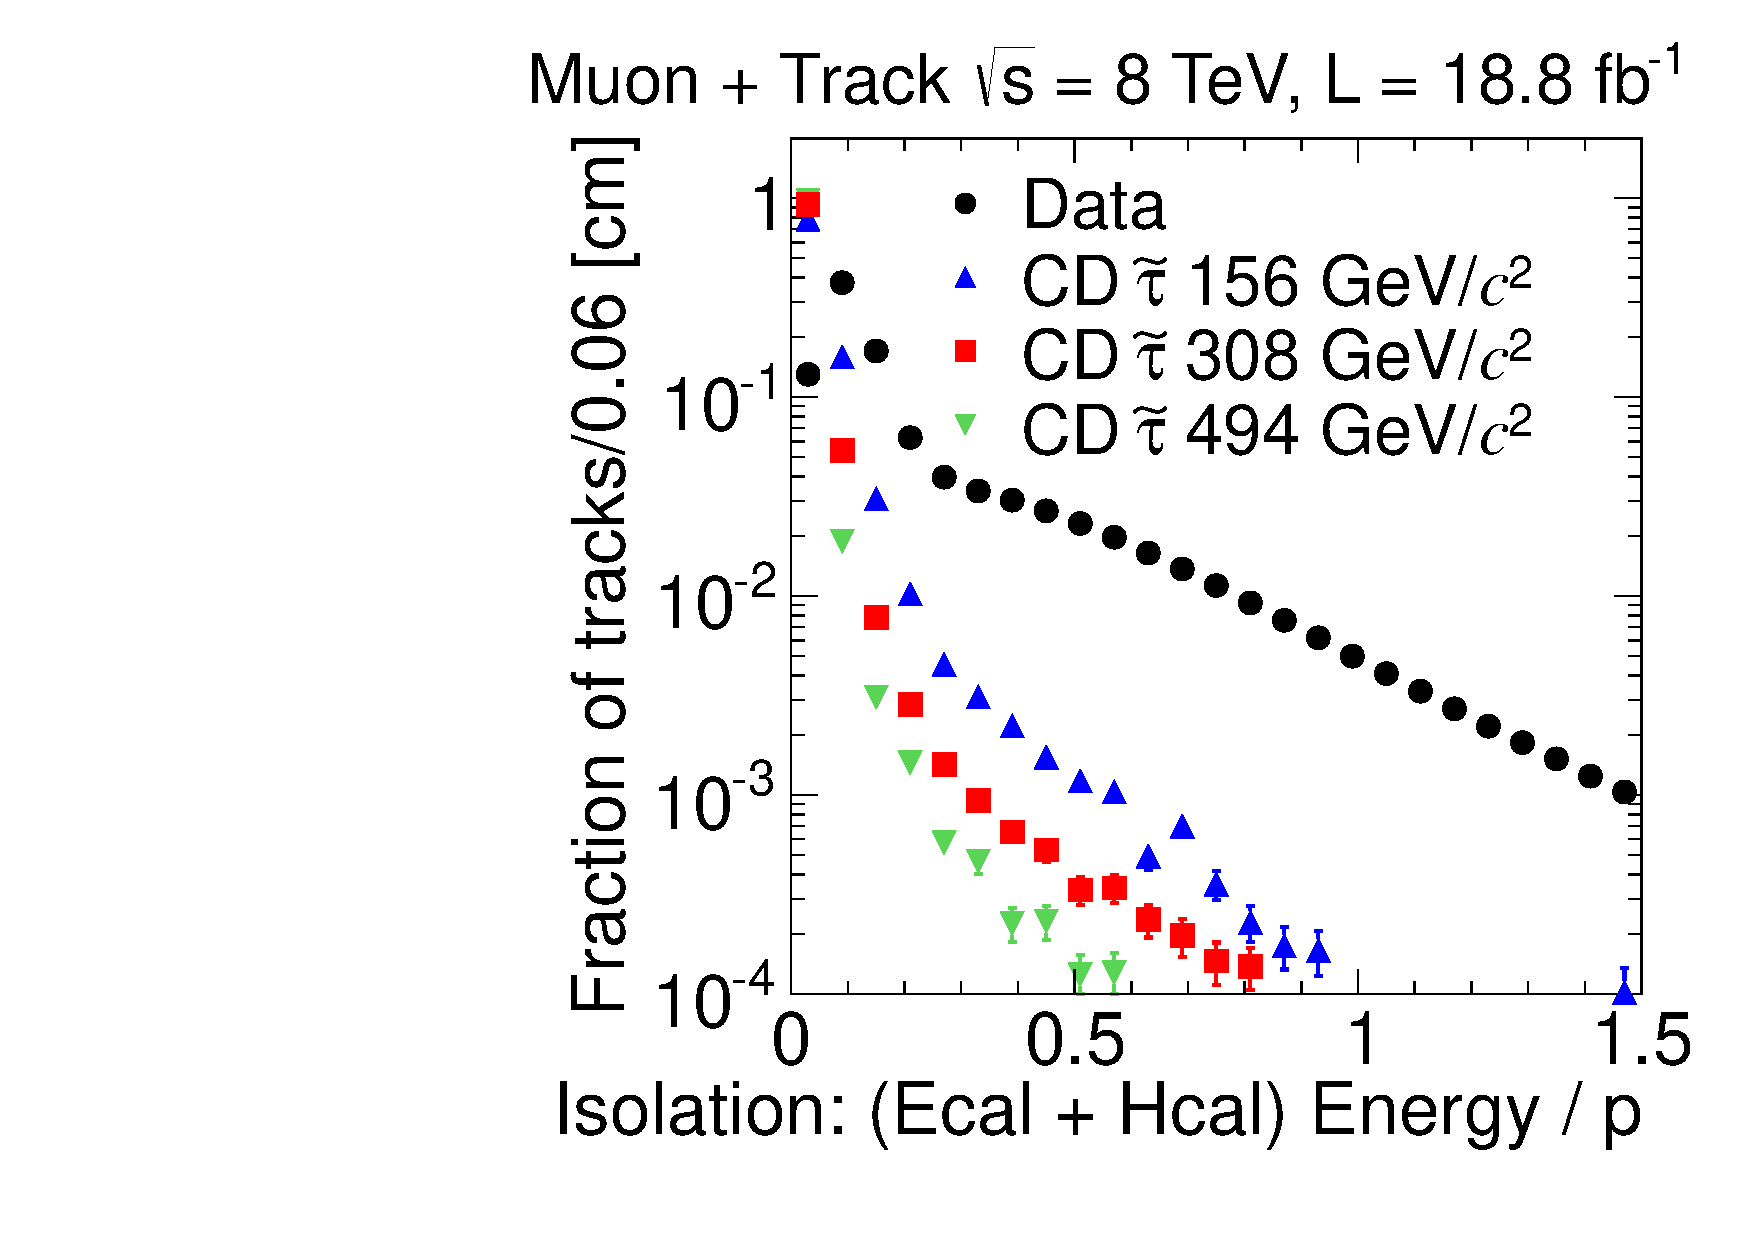
\includegraphics[clip=false, trim=0.0cm 0cm 0.0cm 0cm, width=0.48\textwidth]{figures/tkmu/Selection_Comp_8TeV_GMStau_IsolE_BS} \\
  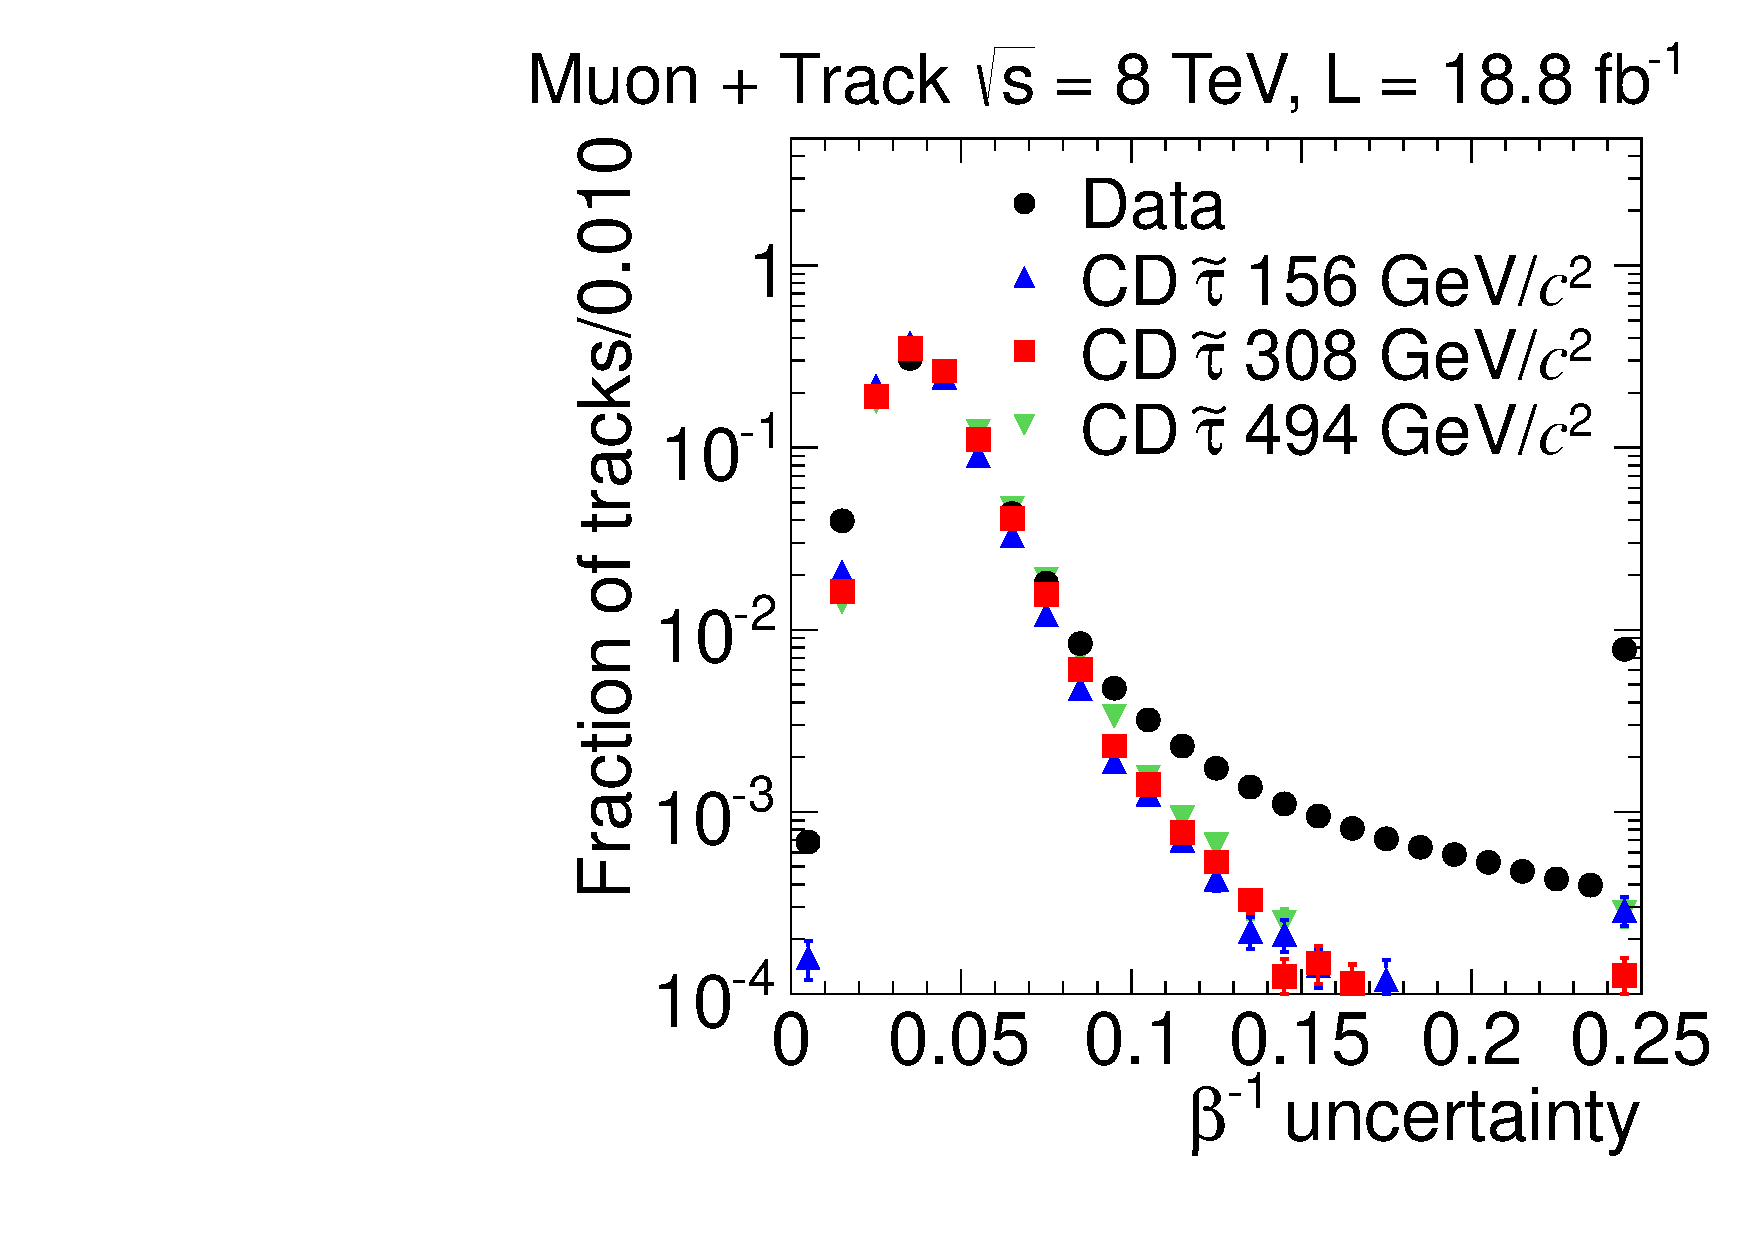
\includegraphics[clip=false, trim=0.0cm 0cm 0.0cm 0cm, width=0.48\textwidth]{figures/tkmu/Selection_Comp_8TeV_GMStau_TOFError_BS}
  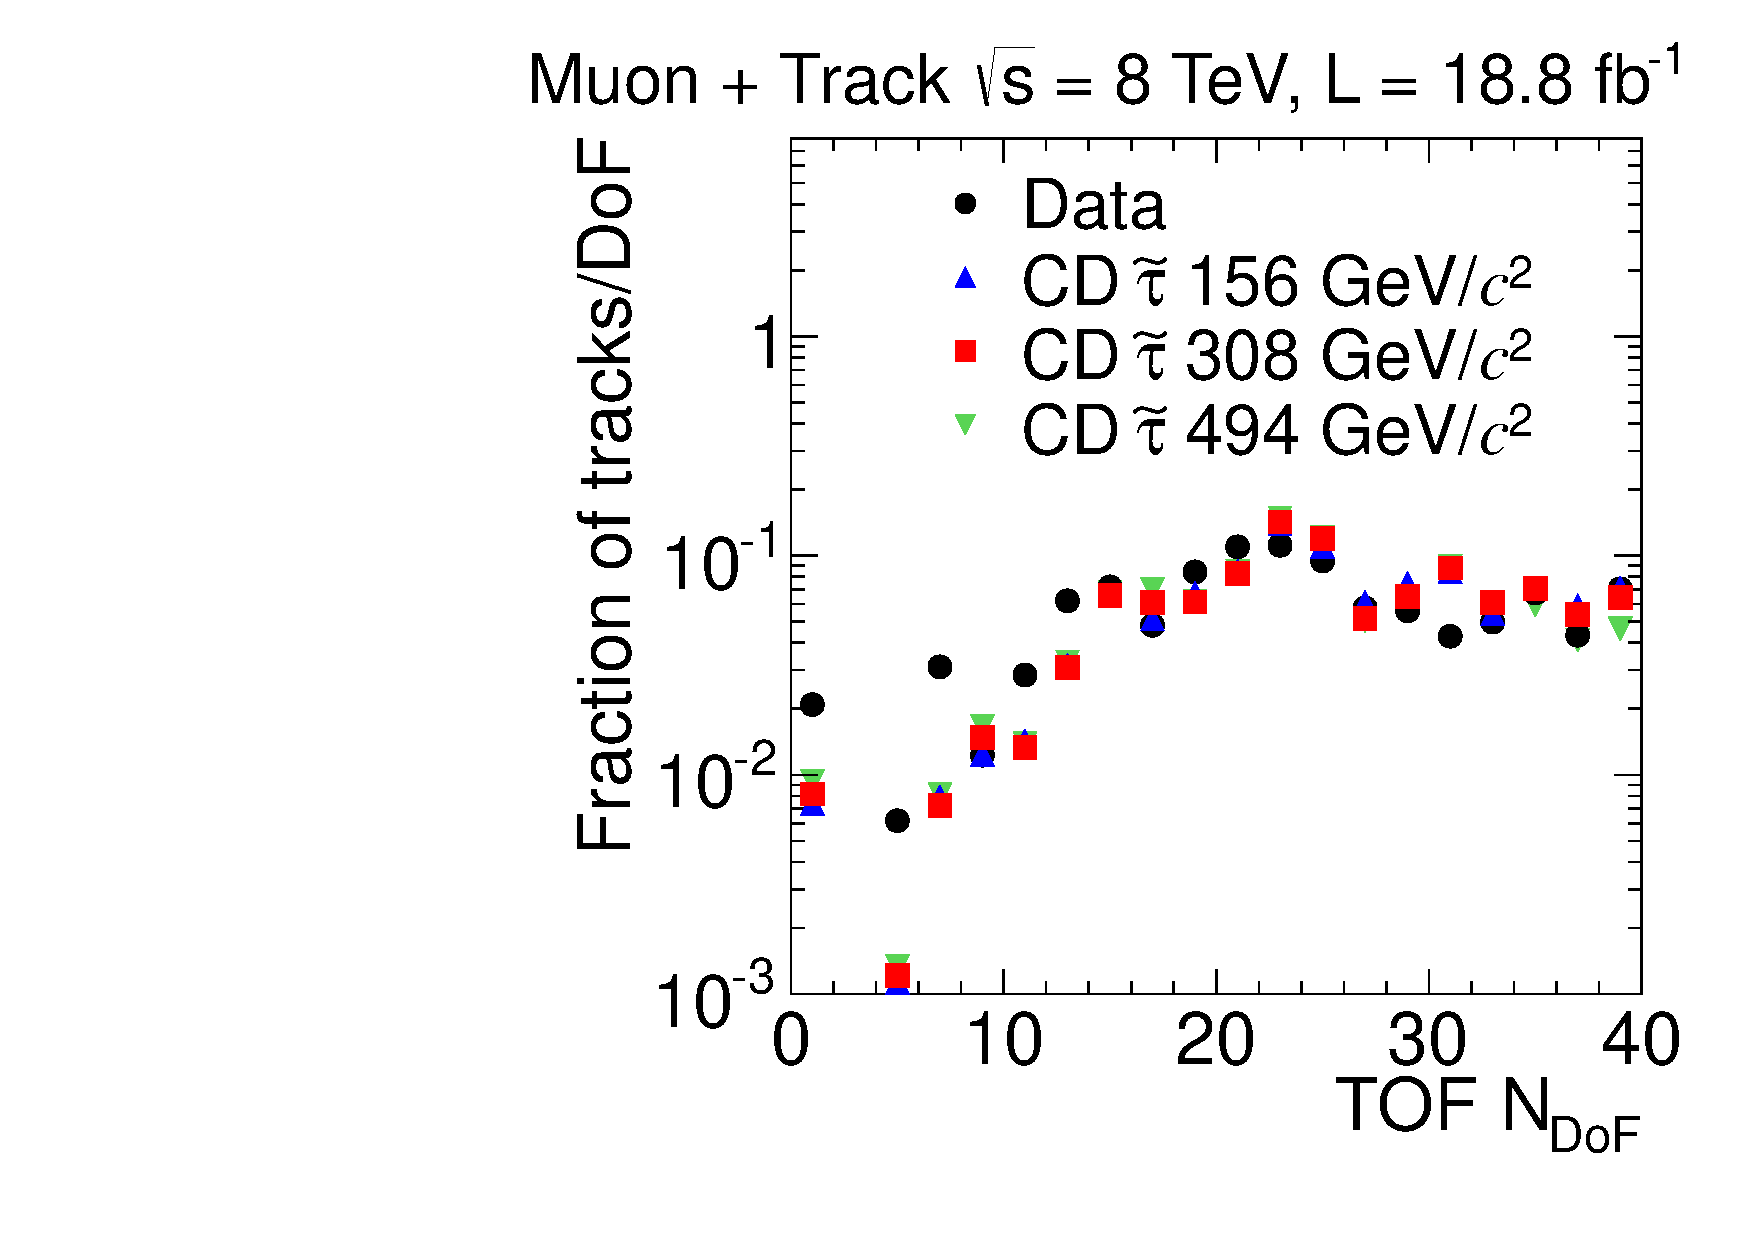
\includegraphics[clip=false, trim=0.0cm 0cm 0.0cm 0cm, width=0.48\textwidth]{figures/tkmu/Selection_Comp_8TeV_GMStau_nDof_BS}
  \caption[Distribution of tracker and calorimeter isolation as well as the \invbeta\ measurement number of degrees of freedom and uncertainty
in the \tktof\ analysis for data and signal MC samples.]
{Distribution of various preselection variables in the \tktof\ analysis for data and signal MC samples.
Top row: Sum momentum of tracks within 0.3 (left) and calorimeter energy within 0.3 divided by track momentum (right).
Bottom row: Distribution of the \invbeta\ measurement uncertainty (left) and the number of degrees of freedom (right).}
    \label{fig:TkMuPreselC}
\end{figure}

\subsection{Preselection for \tkonly\ and \multi\ \label{sec:otherpreselection}}

The \tkonly\ analysis applies the same preselection as the \tktof\ analysis except the cuts on the timing measurement are not applied, as the tracks
are not required to be reconstructed in the muon system. 
%The \fract\ analysis uses preselection like \tkonly\ but inverting the \ih\ requirement
%to be less than 2.8 and requiring no tracks with \pt\ greater than 45 GeV to have an opening angle with the track greater than 2.8 radians.

The \multi\ analysis applies
the same selection criteria as the \tktof\ analysis except the cut on relative isolation less than 0.3 and the cleaning of the hits used for the \dedx\ calculation
is not done. The cleaning procedure is not applied because the amount of charge deposited is proportional to $Q^2$ meaning that even a $Q=2e$ HSCP will
deposit four times as much charge as a $Q=1e$ HSCP. As the tracker saturates for a energy loss approximately three times that expected for a MIP, many of the hits from $Q>1e$ HSCP
will be saturated; this can confuse the cleaning procedure. Additionally, as the high charge samples deposit so much charge, 
there will still be good signal/background separation even with longer tails in the \dedx\ distribution.
Figure~\ref{fig:Multi} shows the number of measurements passing the cleaning for multiply charged samples.
% and the opening angle described above for fractionally charged samples.

\begin{figure}
\centering
%  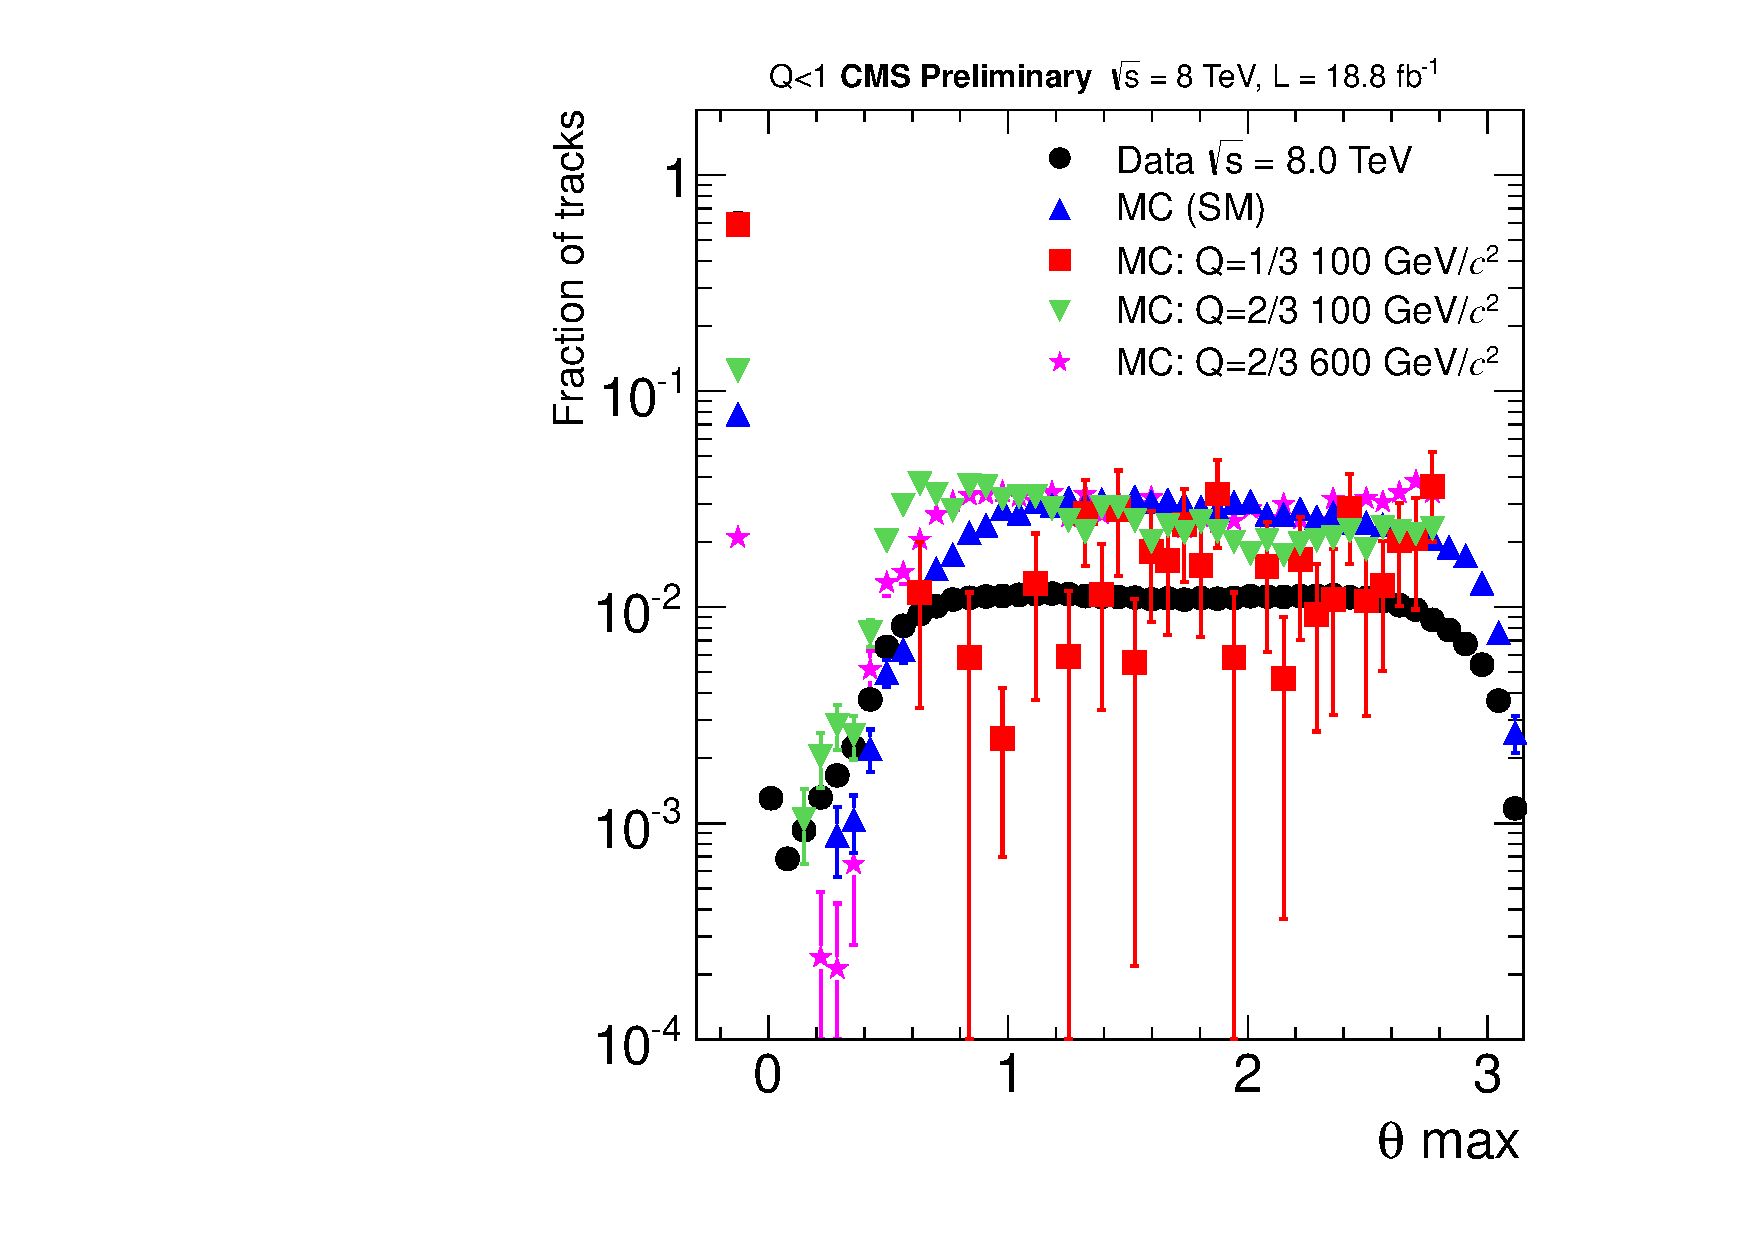
\includegraphics[clip=false, trim=0.0cm 0cm 0.0cm 0cm, width=0.48\textwidth]{figures/fract/Selection_Comp_8TeV_DY_OpenAngle_BS}
  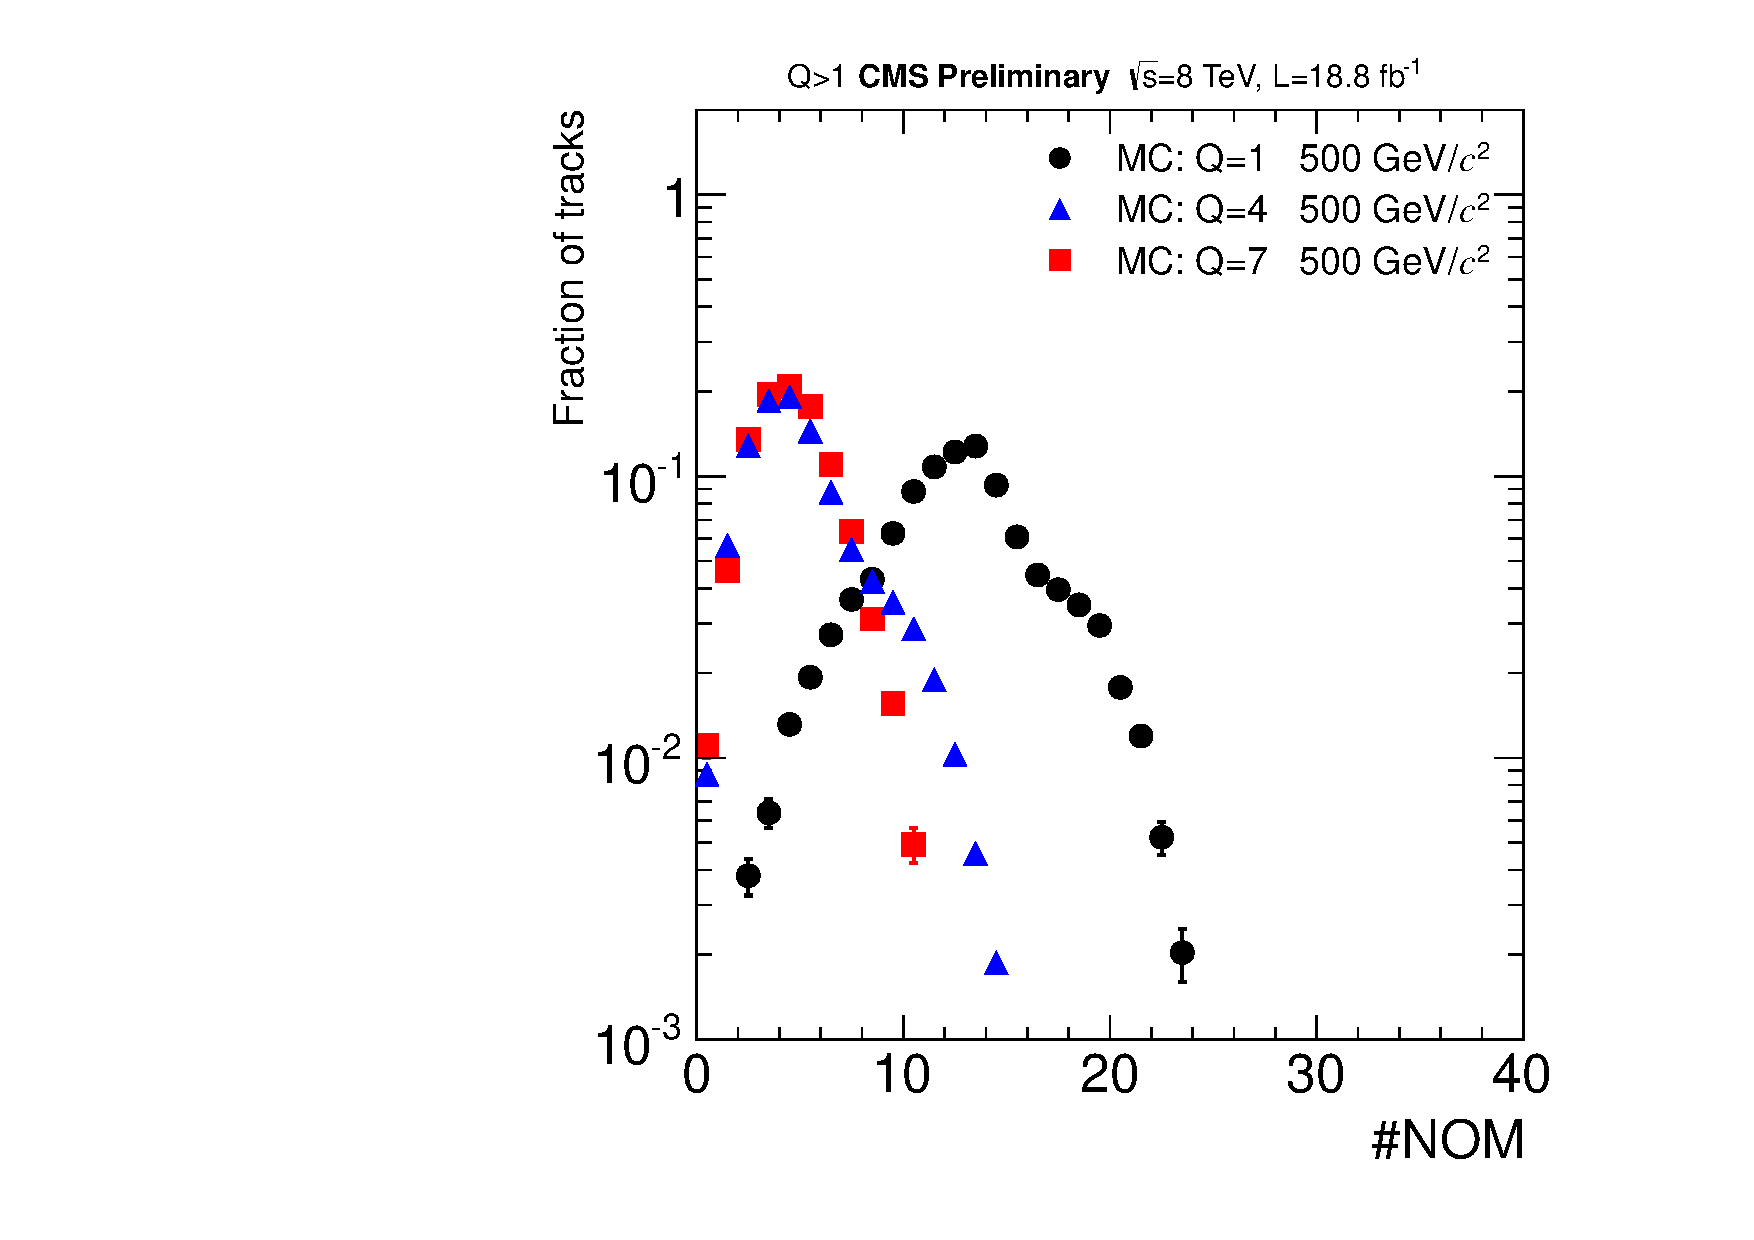
\includegraphics[clip=false, trim=0.0cm 0cm 0.0cm 0cm, width=0.48\textwidth]{figures/multi/Selection_Comp_8TeV_DY_QG_NOM_BS}
  \caption{Distribution of number of \dedx\ measurements passing cleaning for samples of three different charges
    \label{fig:Multi}}
\end{figure}

\subsection{Summary of Preselection \label{sec:summarypreselection}}

The preselection criteria applied on the track in the muon system used in the \muononly, \tktof, and \multi\ analyses are summarized in Table~\ref{tab:preselectionSA}.
The preselection criteria applied on the track in the inner tracker used in the \tktof, \tkonly, and \multi\ analyses are summarized in Table~\ref{tab:preselectionTk}.

%\begin{table}
% \begin{center}
%  \caption{Preselection criteria used in the various analyses}
%     \label{tab:preselection}
%  \begin{tabular}{|l|c|c|c|c|} \hline
%                                            & Muon               & Muon+ & {\em multiple}            & Track       \\
%                                            & Only               & track & {\em charge}              & Only        \\ \hline
%   Track Type                               & Muon               & \multicolumn{2}{c|}{Inner + muon} & Inner       \\ \hline
%   $|\eta|$                                 & \multicolumn{4}{c|}{$< 2.1$}                                         \\ \hline
%   $p_T$ (GeV)                              & $> 80$             & \multicolumn{3}{c|}{$> 45$}                     \\ \hline
%   $d_z$ and $d_{xy}$ (cm)                  & $< 15$             & \multicolumn{3}{c|}{$< 0.5$}                    \\ \hline
%   \# DT or CSC Stations                    & $> 1$              & \multicolumn{3}{c|}{/}                          \\ \hline
%   Opp. segment $|\eta|$ difference         & $> 0.1$            & \multicolumn{3}{c|}{/}                          \\ \hline
%   $|\phi|$                                 & $< 1.2$ OR $> 1.9$ & \multicolumn{3}{c|}{/}                          \\ \hline
%   $|\delta t|$ to other beam crossing (ns) & $> 5$              & \multicolumn{3}{c|}{/}                          \\ \hline
%   \# TOF Measurements                      & \multicolumn{3}{c|}{$> 7$}                             & /           \\ \hline
%   $\sigma_{1/\beta}$                       & \multicolumn{3}{c|}{$< 0.07$}                          & /           \\ \hline
%   $1/\beta$                                & \multicolumn{3}{c|}{$> 1$}                             & /           \\ \hline
%   $\sigma_{p_T}/p_T$                       & /                  & \multicolumn{3}{c|}{$< 0.25$}                   \\ \hline
%   Track $\chi^2/d.o.f$                     & /                  & \multicolumn{3}{c|}{$< 5$}                      \\ \hline
%   \# Pixel Hits                            & /                  & \multicolumn{3}{c|}{$> 1$}                      \\ \hline
%   \# Tracker Hits                          & /                  & \multicolumn{3}{c|}{$> 7$}                      \\ \hline
%   Frac. Valid Hits                         & /                  & \multicolumn{3}{c|}{$> 0.8$}                    \\ \hline
%   \# \dedx\ Measurements                   & /                  & \multicolumn{3}{c|}{$> 5$}                      \\ \hline
%   \ih\ (MeV/cm)                            & /                  & \multicolumn{3}{c|}{ $> 3.0$}                   \\ \hline
%   \dedx\ Strip Shape Test                  & /                  & yes     & no                        & yes       \\ \hline
%   $\Sigma p_T^{trk} (\Delta R < 0.3)$ (GeV)& /                  & \multicolumn{3}{c|}{$< 50$}                     \\ \hline
%   $E_{cal}(\Delta R < 0.3)/p$              & /                  & $< 0.3$ & /                         & $< 0.3$   \\ \hline
%  \end{tabular}
% \end{center}
%\end{table}

\begin{table}
 \begin{center}
  \caption{Summary of preselection criteria on muon system qualities used in the various analyses as defined in the text.
     \label{tab:preselectionSA}}
  \begin{tabular}{|l|c|c|c|} \hline
                                            & \muononly\ & \tktof\  &  $|Q|>1e$    \\ \hline
   \# TOF measurements                      & \multicolumn{3}{c|}{$> 7$}   \\ \hline
   $\sigma_{1/\beta}$                       & \multicolumn{3}{c|}{$< 0.07$}\\ \hline
   $1/\beta$                                & \multicolumn{3}{c|}{$> 1$}   \\ \hline
   $|\eta|$                                 & $< 2.1$              & \multicolumn{2}{c|}{$-$} \\ \hline
   $p_T$ ($GeV/c$)                            & $> 80$      & \multicolumn{2}{c|}{$-$} \\ \hline
   $d_z$ and $d_{xy}$ (cm)                  & $< 15$      & \multicolumn{2}{c|}{$-$} \\ \hline
   \# DT or CSC stations                         & $> 1$      & \multicolumn{2}{c|}{$-$} \\ \hline
   Opp. segment $|\eta|$ difference              & $> 0.1$    & \multicolumn{2}{c|}{$-$} \\ \hline
   $|\phi|$                                      & $< 1.2$ OR $> 1.9$    & \multicolumn{2}{c|}{$-$} \\ \hline
   $|\delta t|$ to other beam crossing (ns)      & $>5$    & \multicolumn{2}{c|}{$-$} \\ \hline
  \end{tabular}
 \end{center}
\end{table}

\begin{table}
 \begin{center}
  \caption{Summary of preselection criteria on the silicon tracker qualities used in the various analyses as defined in the text.
     \label{tab:preselectionTk}}
  \begin{tabular}{|l|c|c|c|} \hline
                                            & \tktof\ & \tkonly\  &  $|Q|>1e$    \\ \hline
   $|\eta|$                                 & \multicolumn{3}{c|}{$< 2.1$}                            \\ \hline
   $p_T$ ($GeV/c$)                            & \multicolumn{3}{c|}{$> 45$}               \\ \hline
   $d_z$ and $d_{xy}$ (cm)                  & \multicolumn{3}{c|}{$< 0.5$}              \\ \hline
   $\sigma_{p_T}/p_T$                       & \multicolumn{3}{c|}{$< 0.25$}             \\ \hline
   Track $\chi^2/{n_d}$           & \multicolumn{3}{c|}{$< 5$}                    \\ \hline
   \# Pixel hits                            & \multicolumn{3}{c|}{$> 1$}                \\ \hline
   \# Tracker hits                          & \multicolumn{3}{c|}{$> 7$}                \\ \hline
   Frac. Valid hits                         & \multicolumn{3}{c|}{$> 0.8$}              \\ \hline
   $\Sigma p_{T}^{trk} (\Delta R < 0.3)$ ($GeV/c$) & \multicolumn{3}{c|}{$< 50$}             \\ \hline
   \# \dedx\ measurements                   & \multicolumn{3}{c|}{$> 5$}                \\ \hline
   \dedx\ strip shape test                  & \multicolumn{2}{c|}{yes}       & no       \\ \hline
   $E_{cal}(\Delta R < 0.3)/p$              & \multicolumn{2}{c|}{$< 0.3$}   & $-$      \\ \hline
  \end{tabular}
 \end{center}
\end{table}

The total preselection efficiency is shown in Tables~\ref{tab:preselectionEff} and ~\ref{tab:preselectionEffA} for the SUSY and modified DY samples, respectively.
The efficiencies are presented with respect to HSCP reconstructed as a track in CMS.
The inefficiency for the \muononly\ analysis mostly arises from the cuts used to suppress the background from cosmic-ray muons.
The other analyses lose efficiency due to quality requirements on the inner track and \dedx\ measurement
which are necessary to constrain the background from misreconstructed tracks.
Additionally, as CMS reconstruction generally assumes signatures of SM particles, HSCP tracks can have a lower quality than a SM particle would.
The requirements are set trying to balance keeping the signal efficiency high while maintaining a low background contamination of the signal region.


\begin{table}
 \begin{center}
  \caption[Preselection efficiency for a few benchmark SUSY samples in the \muononly, \tktof, and \tkonly\ analyses]
{Preselection efficiency for a few benchmark SUSY samples in each analysis.  
This efficiency is with respect to the reconstructed HSCP track (i.e. muon system track for the \muononly\ analysis and muon system plus inner tracker 
for the \tktof\ analysis).
The fraction of glueballs assumed for the gluino samples is given in parentheses at the end of the signal name.}
     \label{tab:preselectionEff}
   \begin{tabular}{|l|c|c|c|} \hline
Model         & \muononly\        & \tktof\        & \tkonly\  \\ \hline
%         & muon-           & track        & track  \\
%Model                    & only           & +muon        & only   \\ \hline
%Gluino 500    & \multirow{2}{*}{44\%} & \multirow{2}{*}{-}    & \multirow{2}{*}{-}  \\
%GeV (1.0)     &                         &                       &                  \\ \hline
%Guino 1000    & \multirow{2}{*}{40\%} & \multirow{2}{*}{-}    & \multirow{2}{*}{-} \\
%GeV (1.0)     &                         &                       &                  \\ \hline
%Gluino 500    & \multirow{2}{*}{44\%} & \multirow{2}{*}{60\%}    & \multirow{2}{*}{70\%} \\
%GeV (0.1)     &                         &                       &                     \\ \hline
%Gluino 1000   & \multirow{2}{*}{43\%} & \multirow{2}{*}{42\%} & \multirow{2}{*}{51\%} \\
%GeV (0.1)     &                         &                       &                     \\ \hline
%Gluino(CS)    & \multirow{2}{*}{-}    & \multirow{2}{*}{-}    & \multirow{2}{*}{64\%} \\
%5500 GeV (0.1) &                       &                       &                       \\ \hline
%Gluino(CS)    & \multirow{2}{*}{-}    & \multirow{2}{*}{-}    & \multirow{2}{*}{47\%} \\
%1000 GeV(0.1) &                         &                       &                     \\ \hline
%Stop 600      & \multirow{2}{*}{48\%} & \multirow{2}{*}{53\%} & \multirow{2}{*}{61\%} \\
%GeV           &                         &                       &                     \\ \hline
%Stop (CS)     & \multirow{2}{*}{56\%} & \multirow{2}{*}{-}    & \multirow{2}{*}{56\%} \\
%600 GeV       &                         &                       &                     \\ \hline
%CD Stau     & \multirow{2}{*}{-}    & \multirow{2}{*}{76\%}    & \multirow{2}{*}{78\%} \\
%370 GeV       &                         &                       &                     \\ \hline%


Gluino 500 GeV (1.0)   & 44\% & -    & -  \\
%GeV (1.0)     &     	      	      	&     	      	      	&     	      	   \\ \hline
Guino 1000 GeV (1.0)   & 40\% & -    & - \\ 
%GeV (1.0)     &     	      	      	&     	      	      	&     	      	   \\ \hline
Gluino 500 GeV (0.1)   & 44\% & 60\%    & 70\% \\
%GeV (0.1)     &     	      	      	&     	      	      	&     	      	      \\ \hline
Gluino 1000 GeV (0.1)  & 43\% & 42\% & 51\% \\
%GeV (0.1)     &     	      	      	&     	      	      	&     	      	      \\ \hline
Gluino(CS) 500 GeV (0.1)   & -    & -    & 64\% \\
%500 GeV (0.1) &                       &                       &                       \\ \hline
Gluino(CS) 1000 GeV (0.1)   & -    & -    & 47\% \\
%1000 GeV(0.1) &     	      	      	&     	      	      	&     	      	      \\ \hline
Stop 600 GeV     & 48\% & 53\% & 61\% \\
%GeV           &     	      	      	&     	      	      	&     	      	      \\ \hline
Stop (CS) GeV    & 56\% & -    & 56\% \\
%600 GeV       &     	      	      	&     	      	      	&     	      	      \\ \hline
CD Stau 370 GeV    & -    & 76\%    & 78\% \\
%370 GeV       &     	      	      	&     	      	      	&     	      	      \\ \hline
\hline
   \end{tabular}
 \end{center}
\end{table}


\begin{table}
 \begin{center}
  \caption
[Preselection efficiency for a few benchmark modified DY samples in the \tktof, \tkonly, and \multi\ analyses.]
{Preselection efficiency for a few benchmark modified DY samples in each analysis.
This efficiency is with respect to the reconstructed HSCP track (i.e. muon system plus inner track for the \multi\ analysis and inner track for the \tkonly\ analysis).}
     \label{tab:preselectionEffA}
   \begin{tabular}{|l|c|c|c|} \hline
%              & track        & track        & {\em multiple} \\
%Model         & +muon        & only         & {\em charge}          \\ \hline
%%DY Q2o3       & \multirow{2}{*}{15\%}    & \multirow{2}{*}{17\%} & \multirow{2}{*}{-} \\
%%400 GeV       &                          &                       &                    \\ \hline
%DY $Q = 1e$         & \multirow{2}{*}{72\%}    & \multirow{2}{*}{76\%} & \multirow{2}{*}{75\%} \\
%600 GeV       &                          &                       &                       \\ \hline
%DY $Q = 3e$         & \multirow{2}{*}{-}    & \multirow{2}{*}{-}    & \multirow{2}{*}{71\%} \\
%600 GeV       &                          &                       &                       \\ \hline
%DY $Q = 5e$         & \multirow{2}{*}{-}    & \multirow{2}{*}{-}    & \multirow{2}{*}{50\%} \\
%600 GeV       &                          &                       &                       \\ \hline
%DY $Q 7e$         & \multirow{2}{*}{-}       & \multirow{2}{*}{-}    & \multirow{2}{*}{37\%} \\
%600 GeV       &                          &                       &                       \\ \hline

Model     & \tktof\    & \tkonly\        & \multi\ \\ \hline
DY $Q = 1e$ 600 GeV        & 72\%    & 76\% & 75\% \\
DY $Q = 3e$ 600 GeV        & -    & -    & 71\% \\
DY $Q = 5e$ 600 GeV        & -    & -    & 50\% \\
DY $Q = 7e$ 600 GeV        & -       & -    & 37\% \\
\hline
   \end{tabular}
 \end{center}
\end{table}


The distributions of $p_T$ and \invbeta\ for the \muononly\ analysis for data, cosmic-ray muon control sample, and various signal models is 
shown in Figure~\ref{fig:MuOnlySelVar} after applying the preselection requirements. Figure~\ref{fig:TkMuSelVar} shows the $p_T$, \invbeta, and \dedx\
distributions after applying the \tktof\ preselection cuts for data and various signal models.

\begin{figure}
\centering
  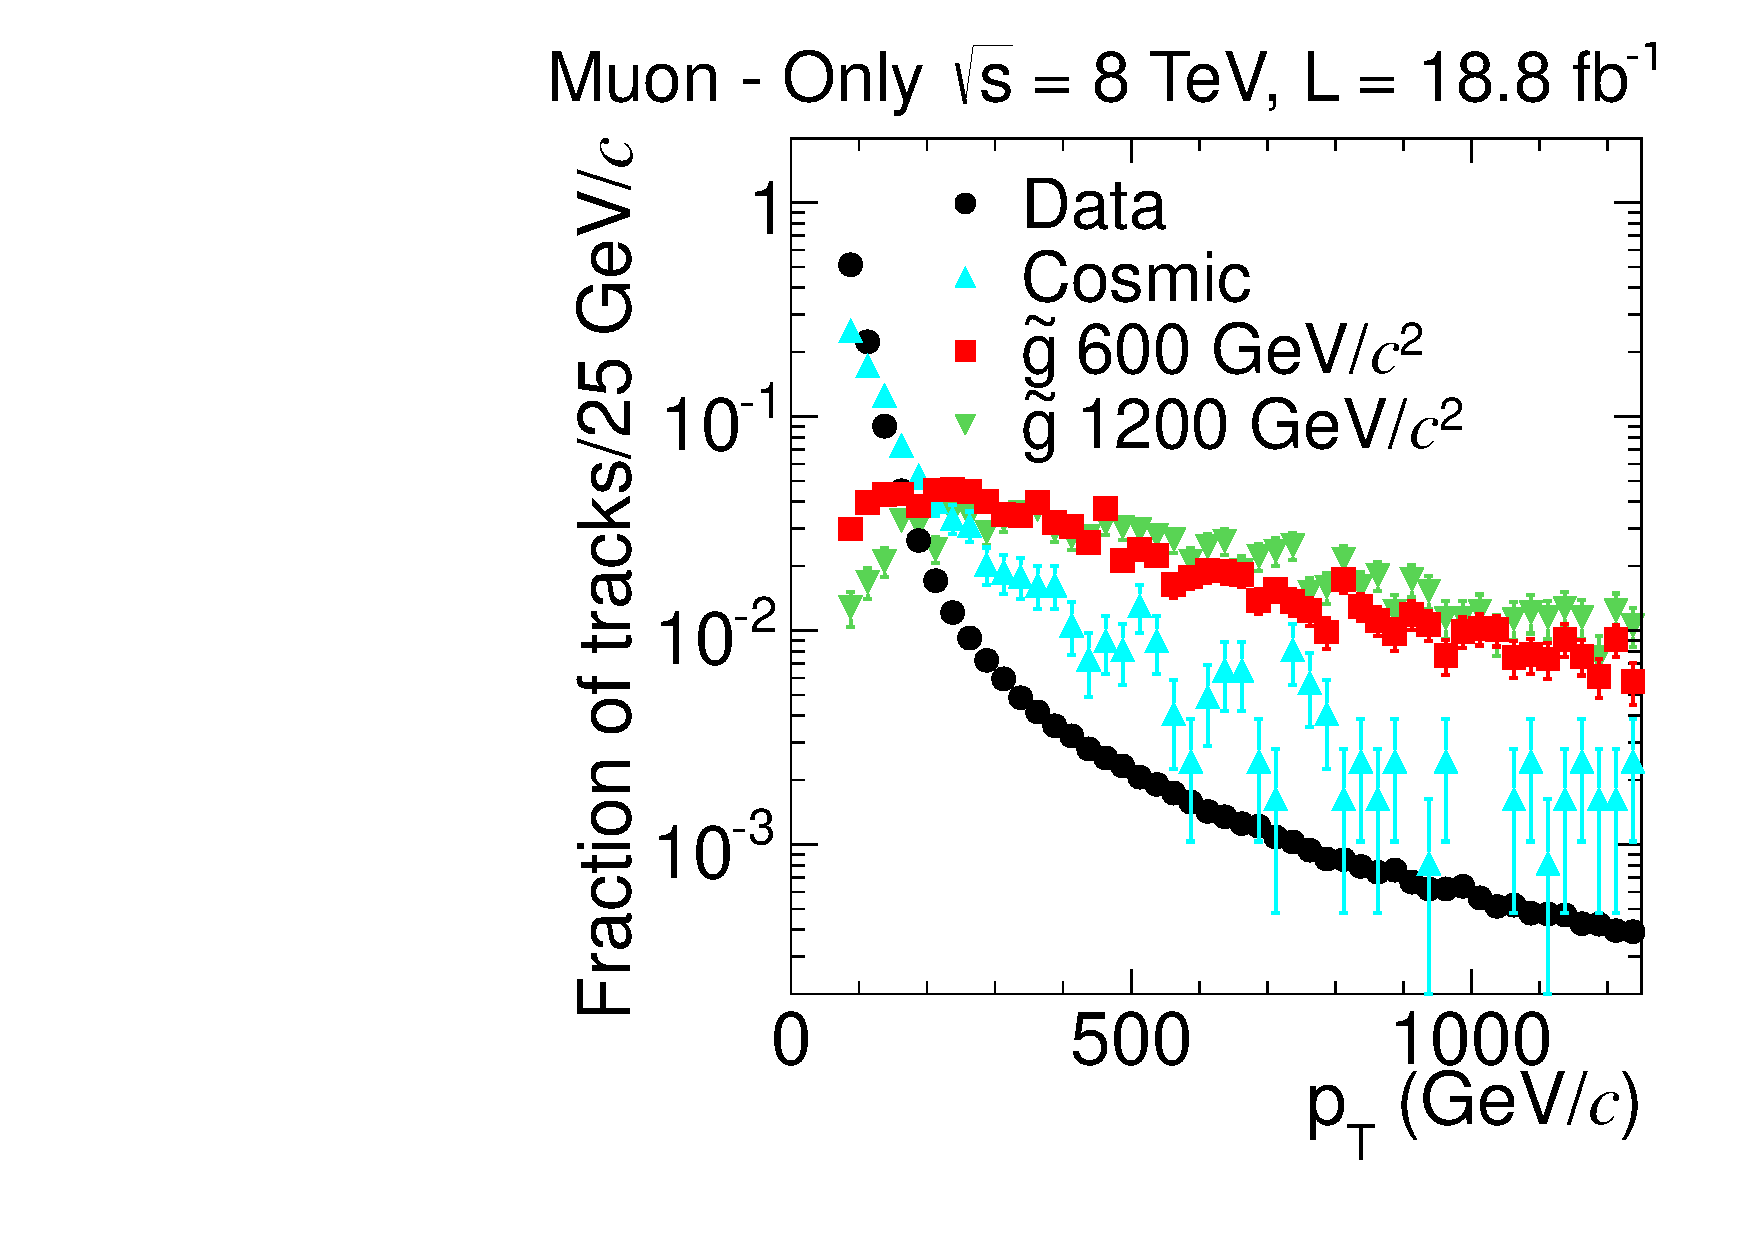
\includegraphics[clip=false, trim=0.0cm 0cm 0.0cm 0cm, width=0.48\textwidth]{figures/muonly/Selection_Comp_8TeV_Cosmic_Pt_BS}
  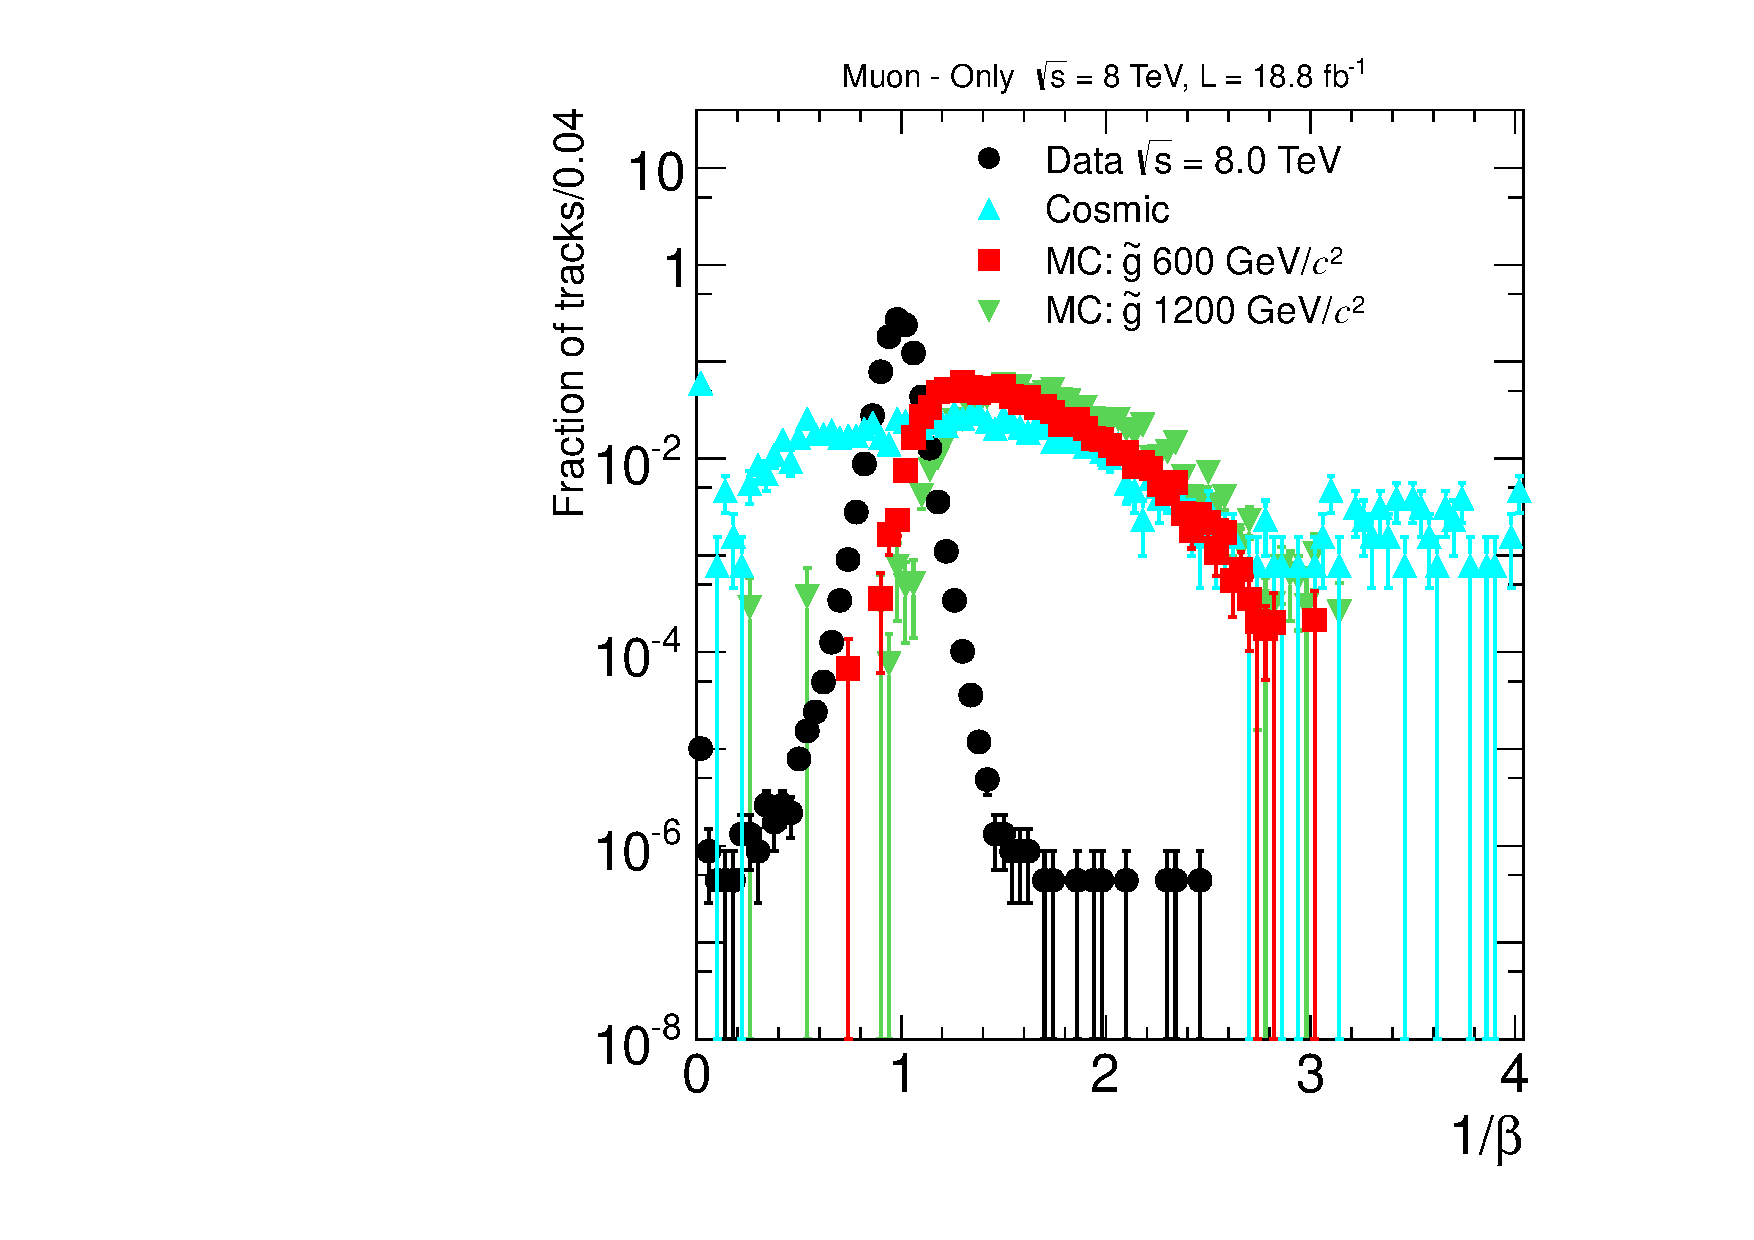
\includegraphics[clip=false, trim=0.0cm 0cm 0.0cm 0cm, width=0.48\textwidth]{figures/muonly/Selection_Comp_8TeV_Cosmic_TOF_BS} \\
  \caption[Distribution of \invbeta\ and \pt\ in the \muononly\ analysis for data, cosmic-ray muon control sample, and signal MC samples]
{Distribution of selection variables for data, cosmic-ray muon control sample, and signal MC samples.
Left: Distribution of $p_T$. Right: Distribution of \invbeta.}
    \label{fig:MuOnlySelVar}
\end{figure}

\begin{figure}
\centering
  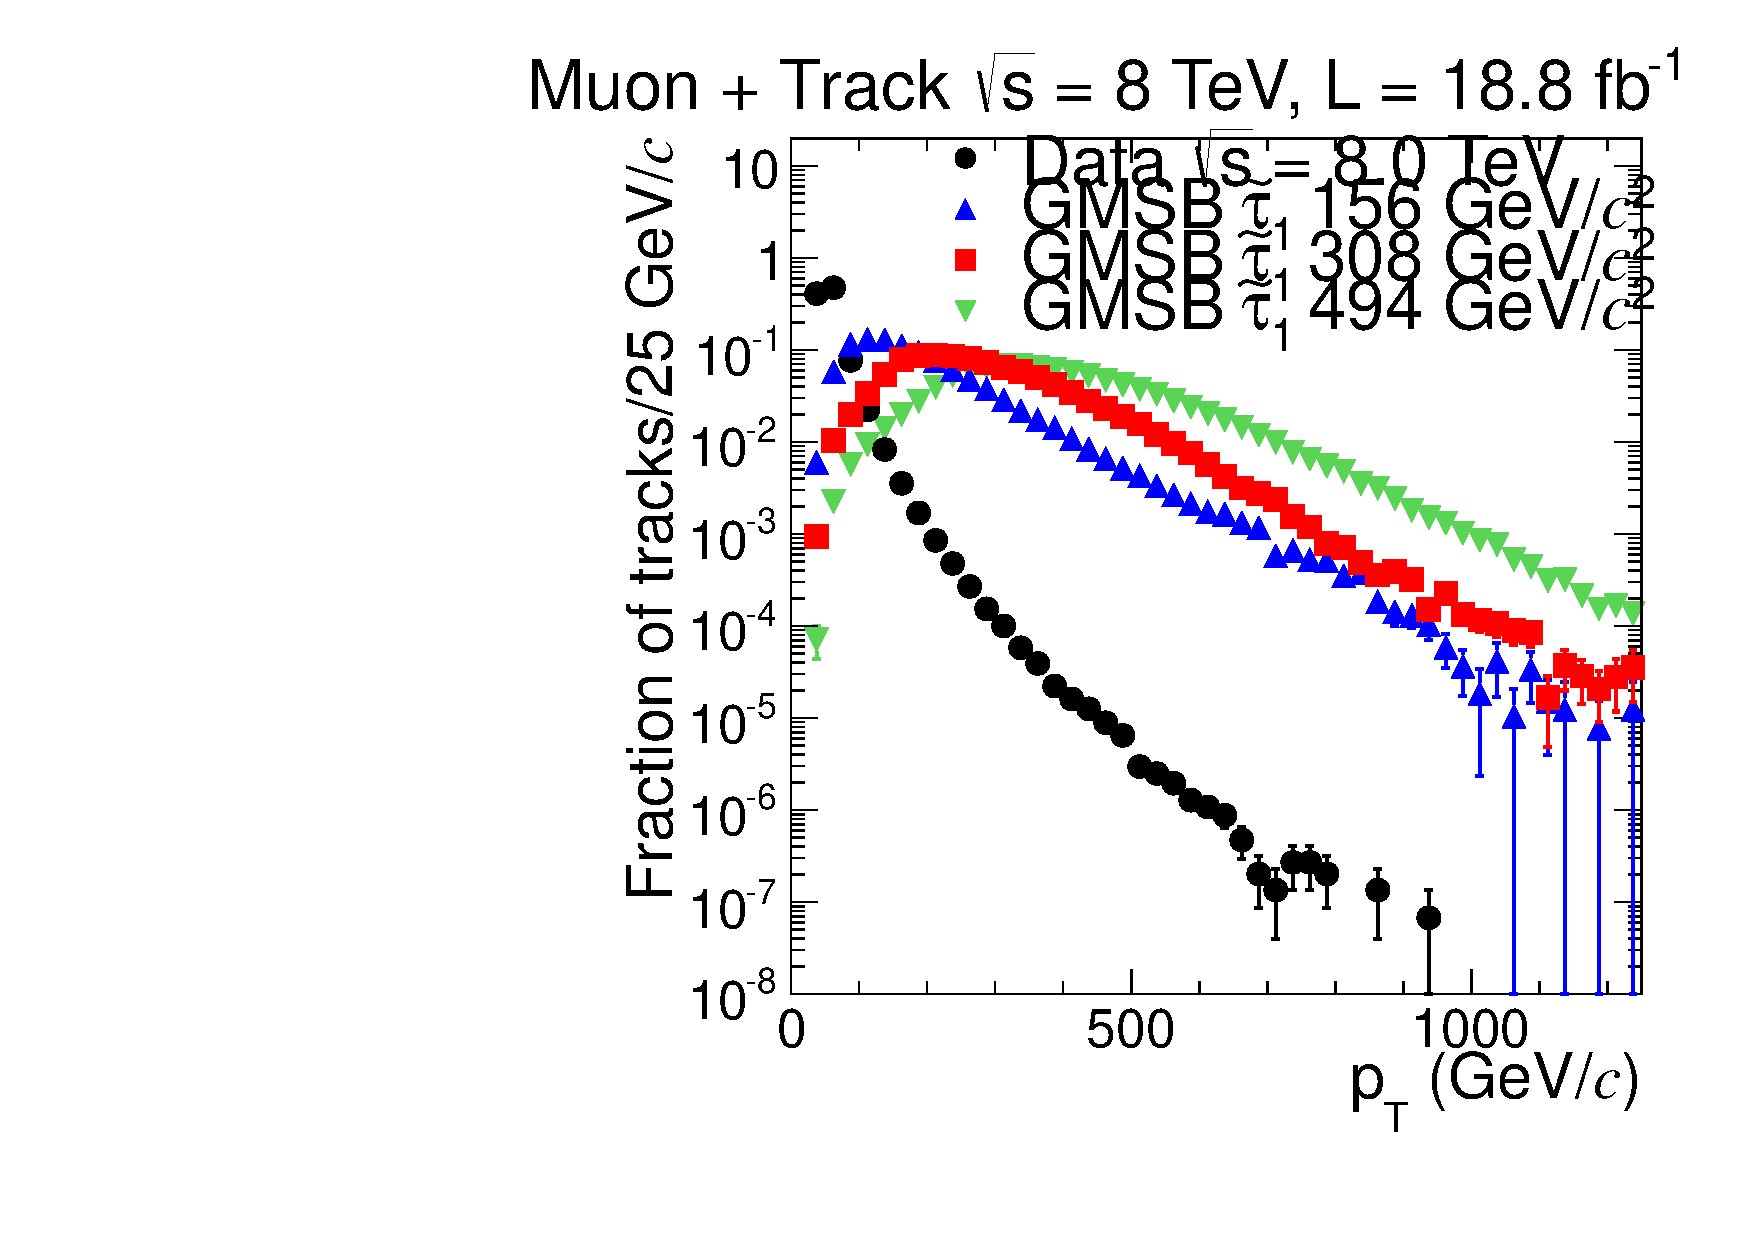
\includegraphics[clip=false, trim=0.0cm 0cm 0.0cm 0cm, width=0.48\textwidth]{figures/tkmu/Selection_Comp_8TeV_GMStau_Pt_BS}
  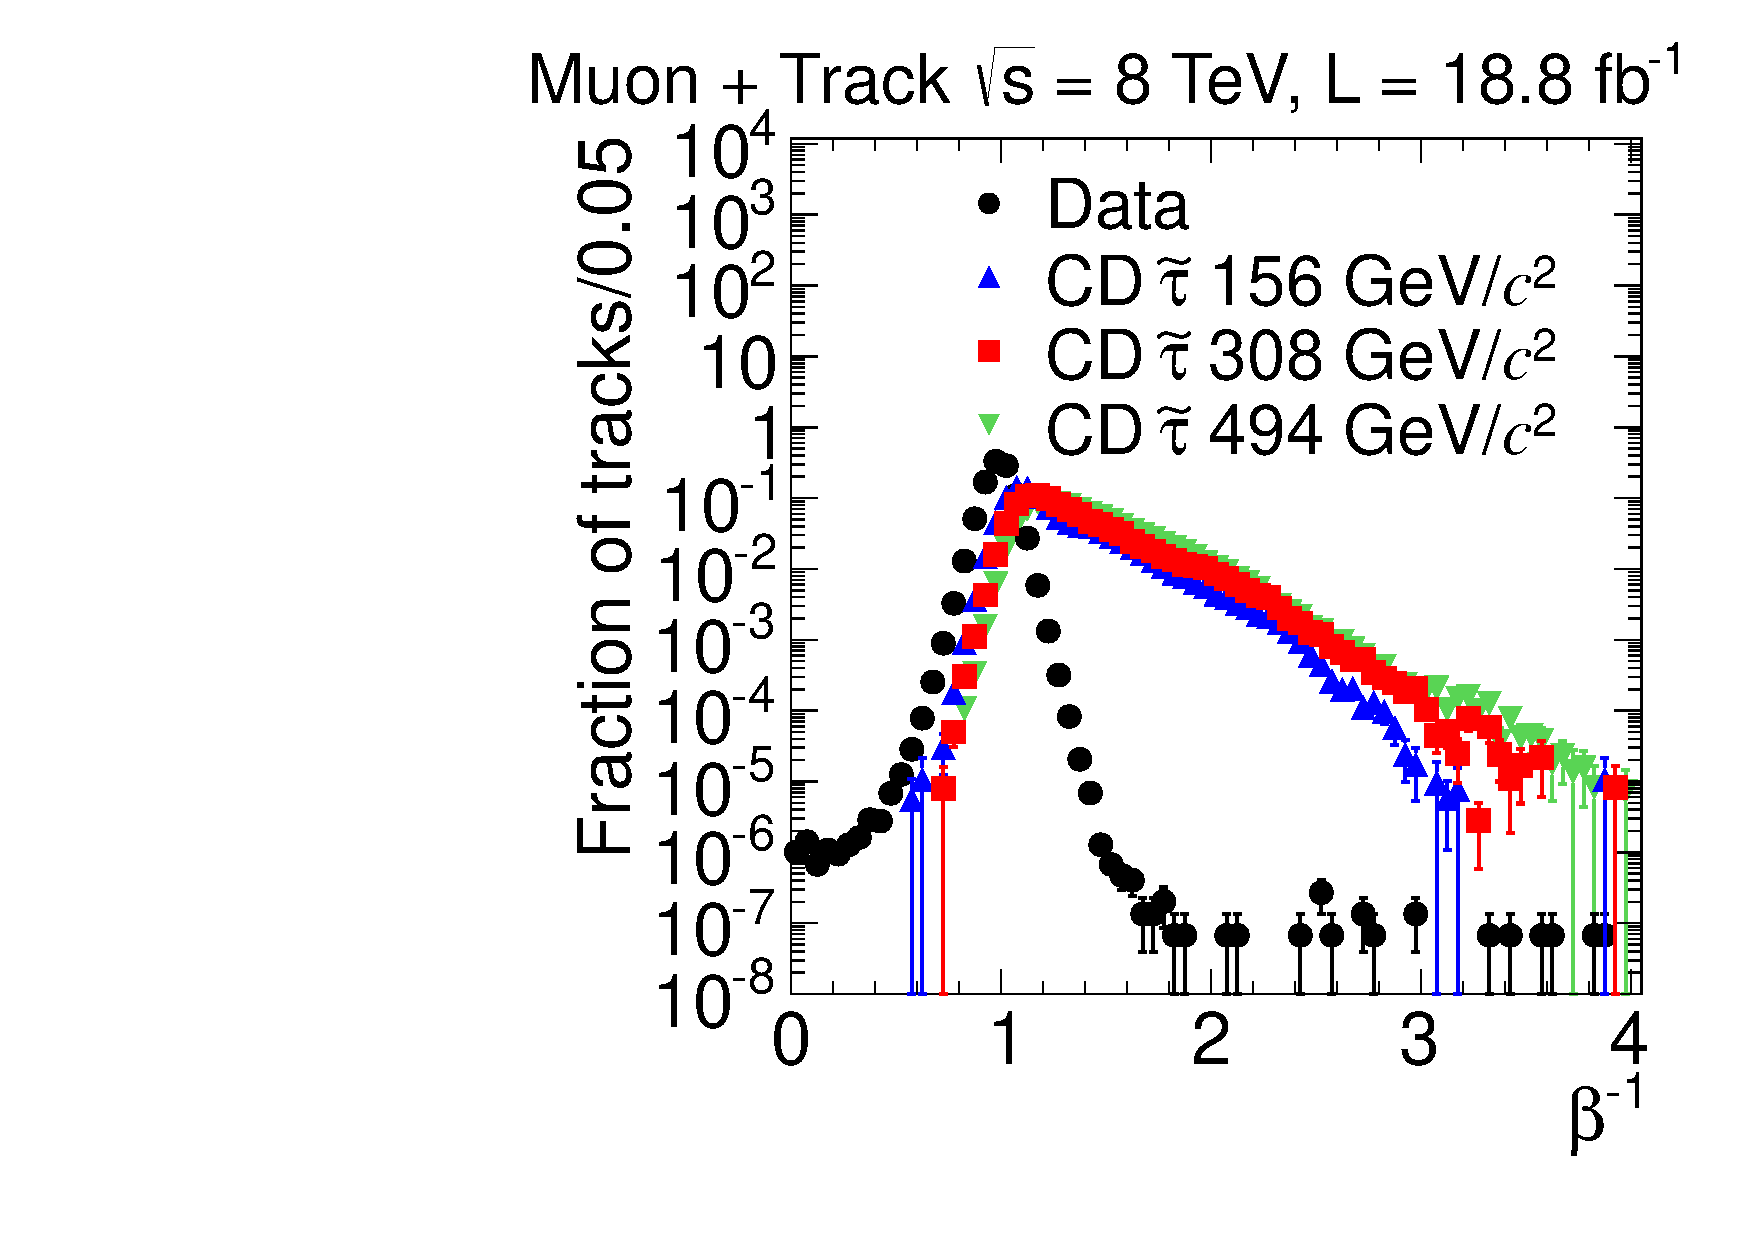
\includegraphics[clip=false, trim=0.0cm 0cm 0.0cm 0cm, width=0.48\textwidth]{figures/tkmu/Selection_Comp_8TeV_GMStau_TOF_BS} \\
  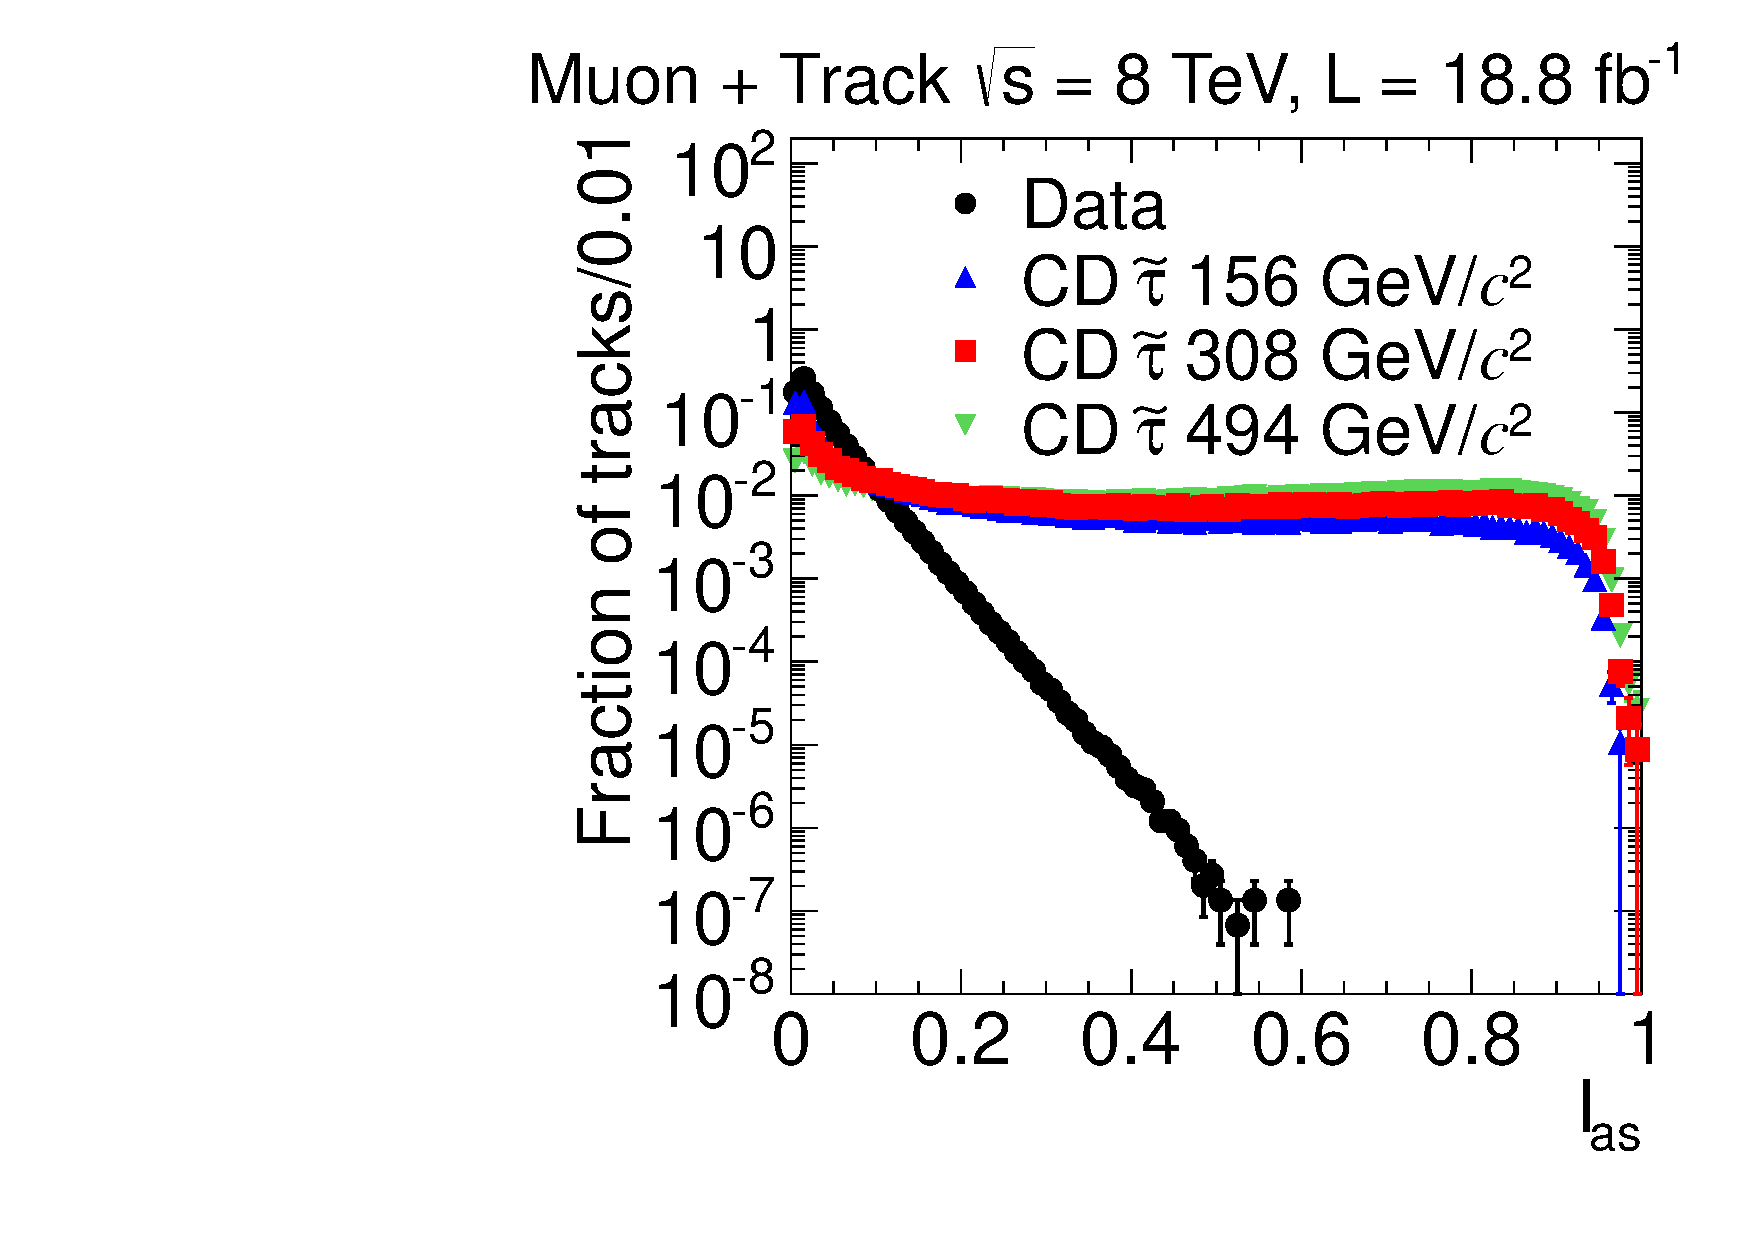
\includegraphics[clip=false, trim=0.0cm 0cm 0.0cm 0cm, width=0.48\textwidth]{figures/tkmu/Selection_Comp_8TeV_GMStau_Is_BS}
  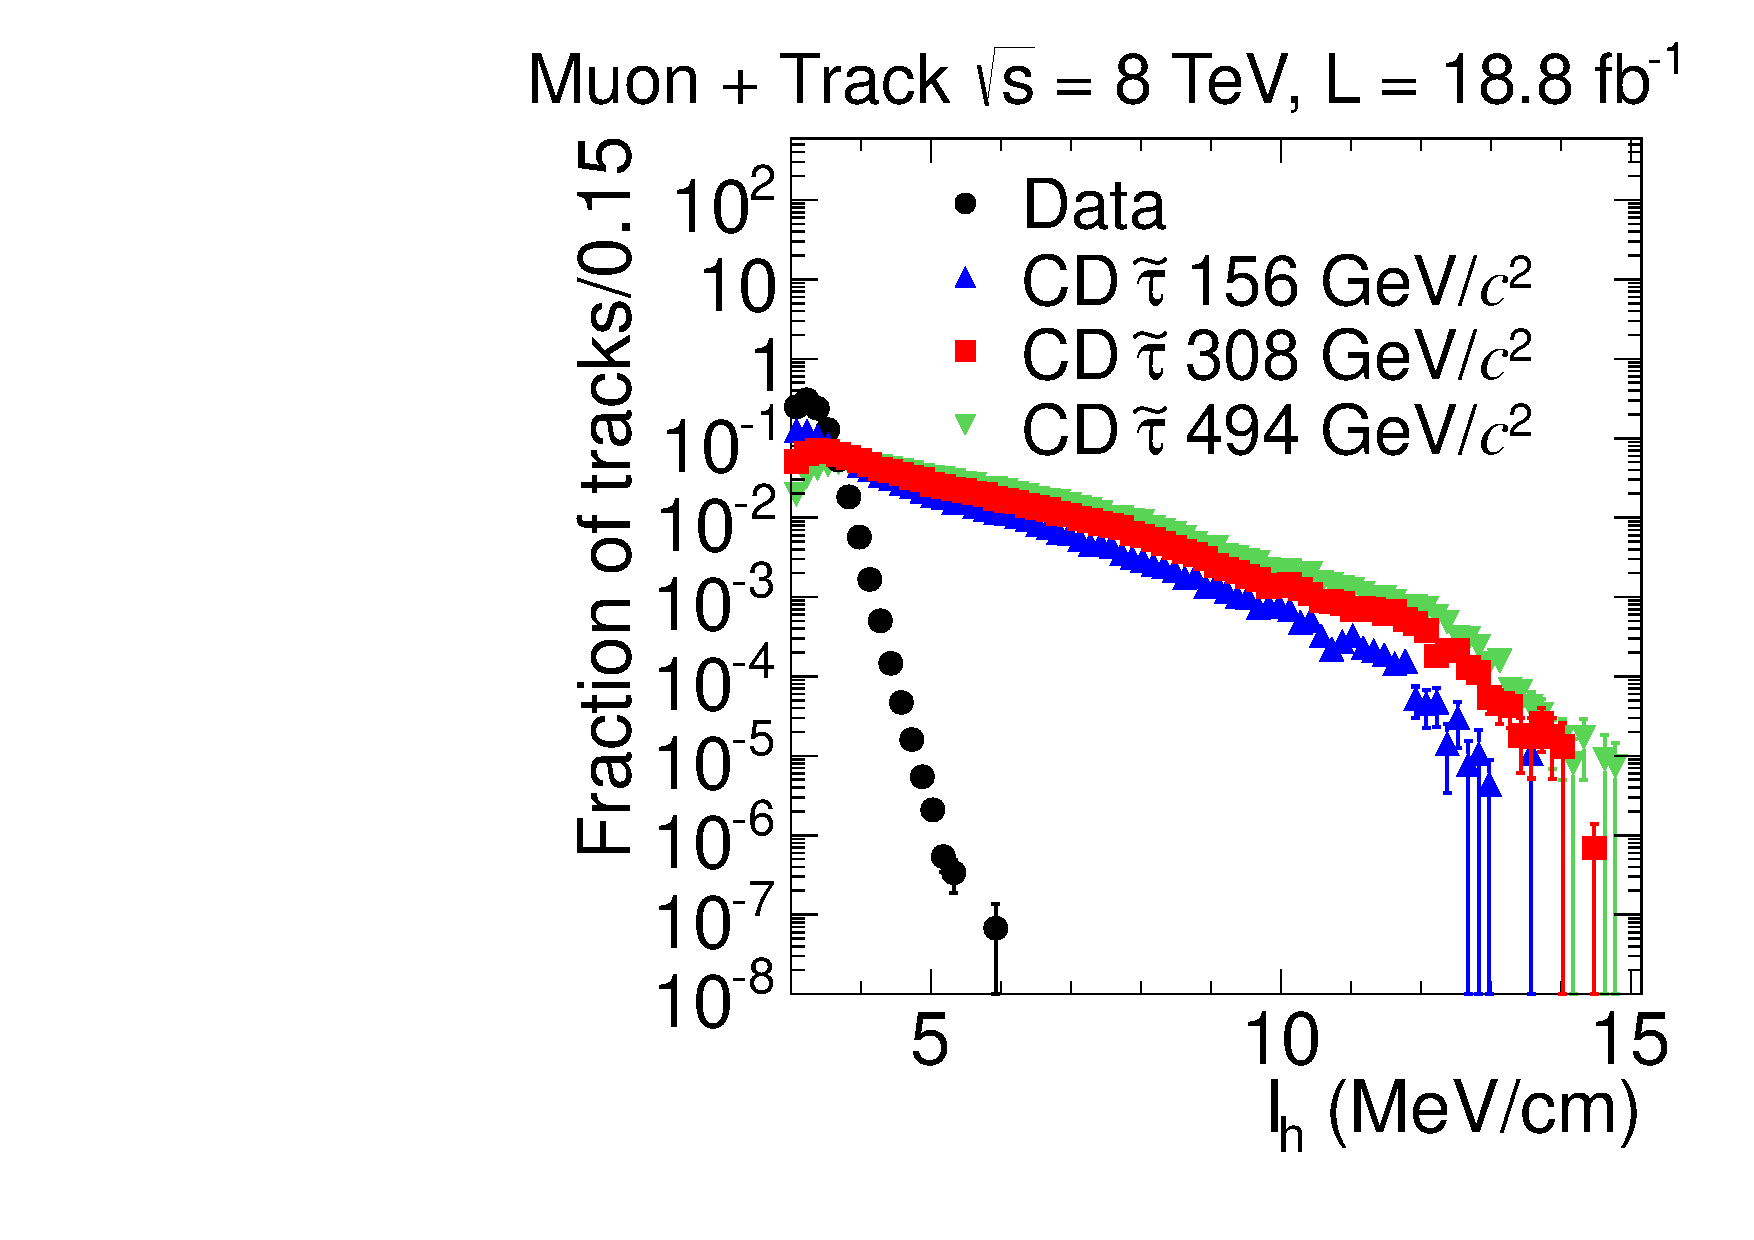
\includegraphics[clip=false, trim=0.0cm 0cm 0.0cm 0cm, width=0.48\textwidth]{figures/tkmu/Selection_Comp_8TeV_GMStau_Im_BS}
  \caption[Distribution of selection variables in the \tktof\ analysis for data and signal MC samples.]
{Distribution of section variables for data and signal MC samples.
Top row: Distribution of $p_T$ (left) and \invbeta\ (right).
Bottom row: Distribution of \ias\ (left) and \ih\ (right).}
    \label{fig:TkMuSelVar}
\end{figure}

\subsection{Tag and Probe Studies \label{sec:TagProbe}}
The study of the agreement between data and MC simulation for numerous muon qualities is done by the Muon POG of CMS.
The group provides scale factors for correcting MC samples to match data.
For all of the analyses except for \muononly\  it is sufficient to use results obtained from this group as the muon qualities
those analyses use are common within CMS.
However, as the \muononly\ analysis uses numerous variables which are unique to it, the results from the muon POG are not applicable to it.

For this reason, additional studies were performed to test the agreement of MC simulation with data.
The efficiency of the selections was checked with a tag-and-probe technique~\cite{2012JInst...7P0002T} using muons from Z boson decays.
% Z bosons decay to a particle and its anti-particle with the invariant mass of the particle--anti-particle
%pair equal to the mass of the Z boson they were created from.
The tag-and-probe procedure proceeds by requiring one muon, the ``tag'' muon, be found with a stringent selection while the other muon, the ``probe'' muon,
is required to be found with only a loose selection using only the silicon tracker. The efficiency to pass the preselection in the \muononly\ analysis
can then be estimated as the fraction of of the probes that pass the preselection. The background from processes other than Z bosons is small and is subtracted by
a simultaneous fit to the tag-probe invariant mass distributions of signal and background around the Z boson mass.
The efficiency estimated in data is compared with that found in MC samples. Scale factors are used to correct the MC samples for any discrepancy observed between the efficiencies.
The MC sample used does not contain any production from background processes.

The tag muon is required to pass the tight selection (see Section.~\ref{sec:timingintro}) recommended by the Muon POG and to match to an object that triggered the read out of CMS. 
The last requirement assures that no bias is introduced in the efficiency measurement by the need for the event to have been read out.
Additionally, the tag must pass the requirements of a skim that was used to reduce the data size to a level
making processing reasonable. The skim requirements are at least three \dedx\ measurements and \ih\ $> 3.0$ or \ih\ $< 2.8$.

A set of probe candidates is defined as tracks reconstructed in the inner tracker with no requirement
of muon system activity. The probes are required to have $p_T > 40$ GeV, $|\eta| < 2.1$, and the opposite charge of the tag muon.
The invariant mass of the tag-probe pair is then required to be within 10 GeV of the mass of the Z boson, 91 GeV.
The invariant mass distribution of the tag-probe pairs is fit using the
sum of two Voigtians (the convolution of a Lorentzian and a Gaussian) to represent the signal and an exponential for the background.

%The fit is found to agree well with the data.
%Figures~\ref{fig:MuOnlyTagProbeFitData} and ~\ref{fig:MuOnlyTagProbeFitMC} show sample fits to data and MC, respectively.
%It can be seen that the fits match well.
%The efficiency is extracted from these fits using a procedure from the muon POG.

%\begin{figure}
% \begin{center}
%  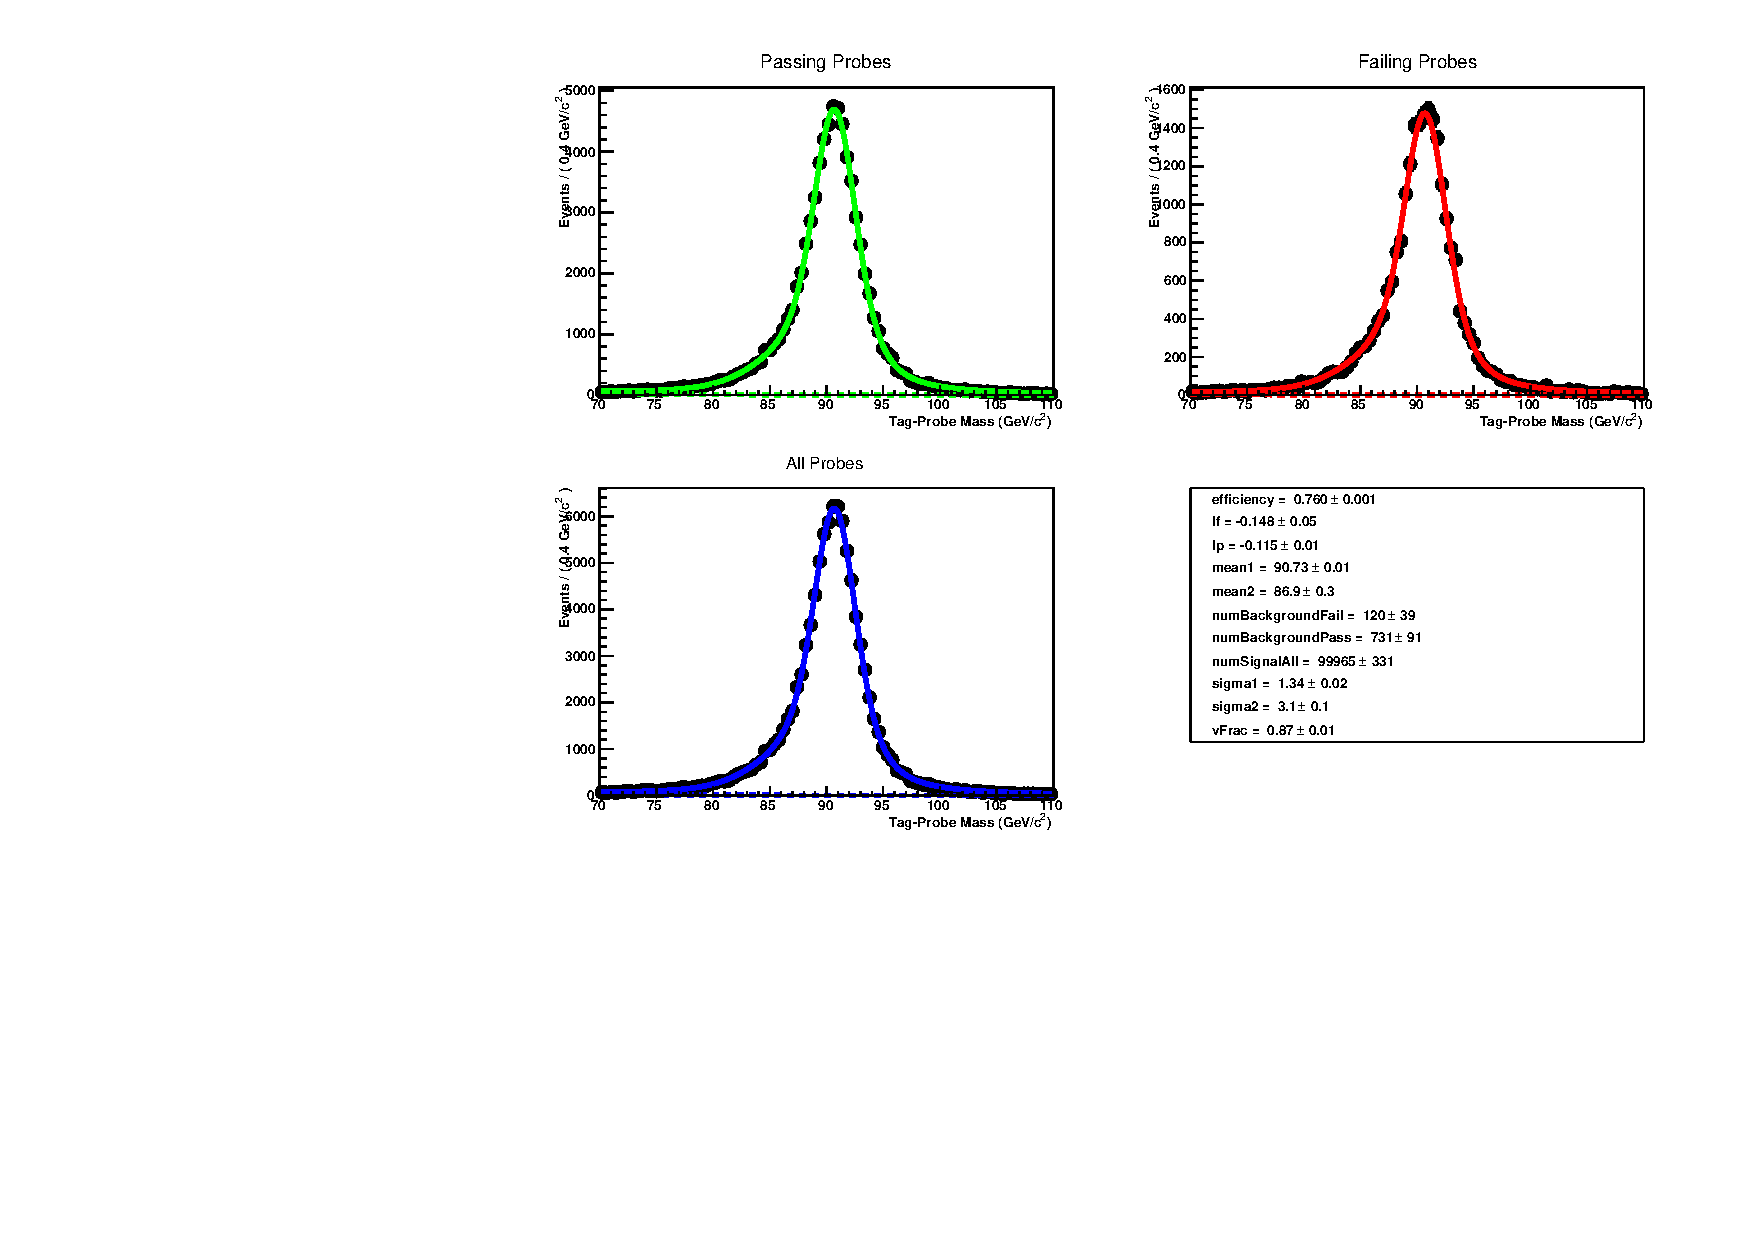
\includegraphics[clip=true, trim=0.0cm 7.0cm 0.0cm 0.0cm, width=0.95\textwidth]{figures/muonly/FitCanvasDataPtBin0}
% \end{center}
% \caption[Example fits to invariant mass distributions
%in the tag-and-probe procedure for the \muononly\ analysis for data.]
%{Example fits to invariant mass distributions
%in the tag-and-probe procedure for the \muononly\ analysis for data.
%Top left: Mass distribution and fit for probes passing the preselection. Top right: Mass distribution and fit for probes failing the preselection.
%Bottom left: Mass distribution and fit for all probes. Bottom right: Parameters extracted from the fit.}
%    \label{fig:MuOnlyTagProbeFitData}
%\end{figure}

%\begin{figure}
% \begin{center}
%  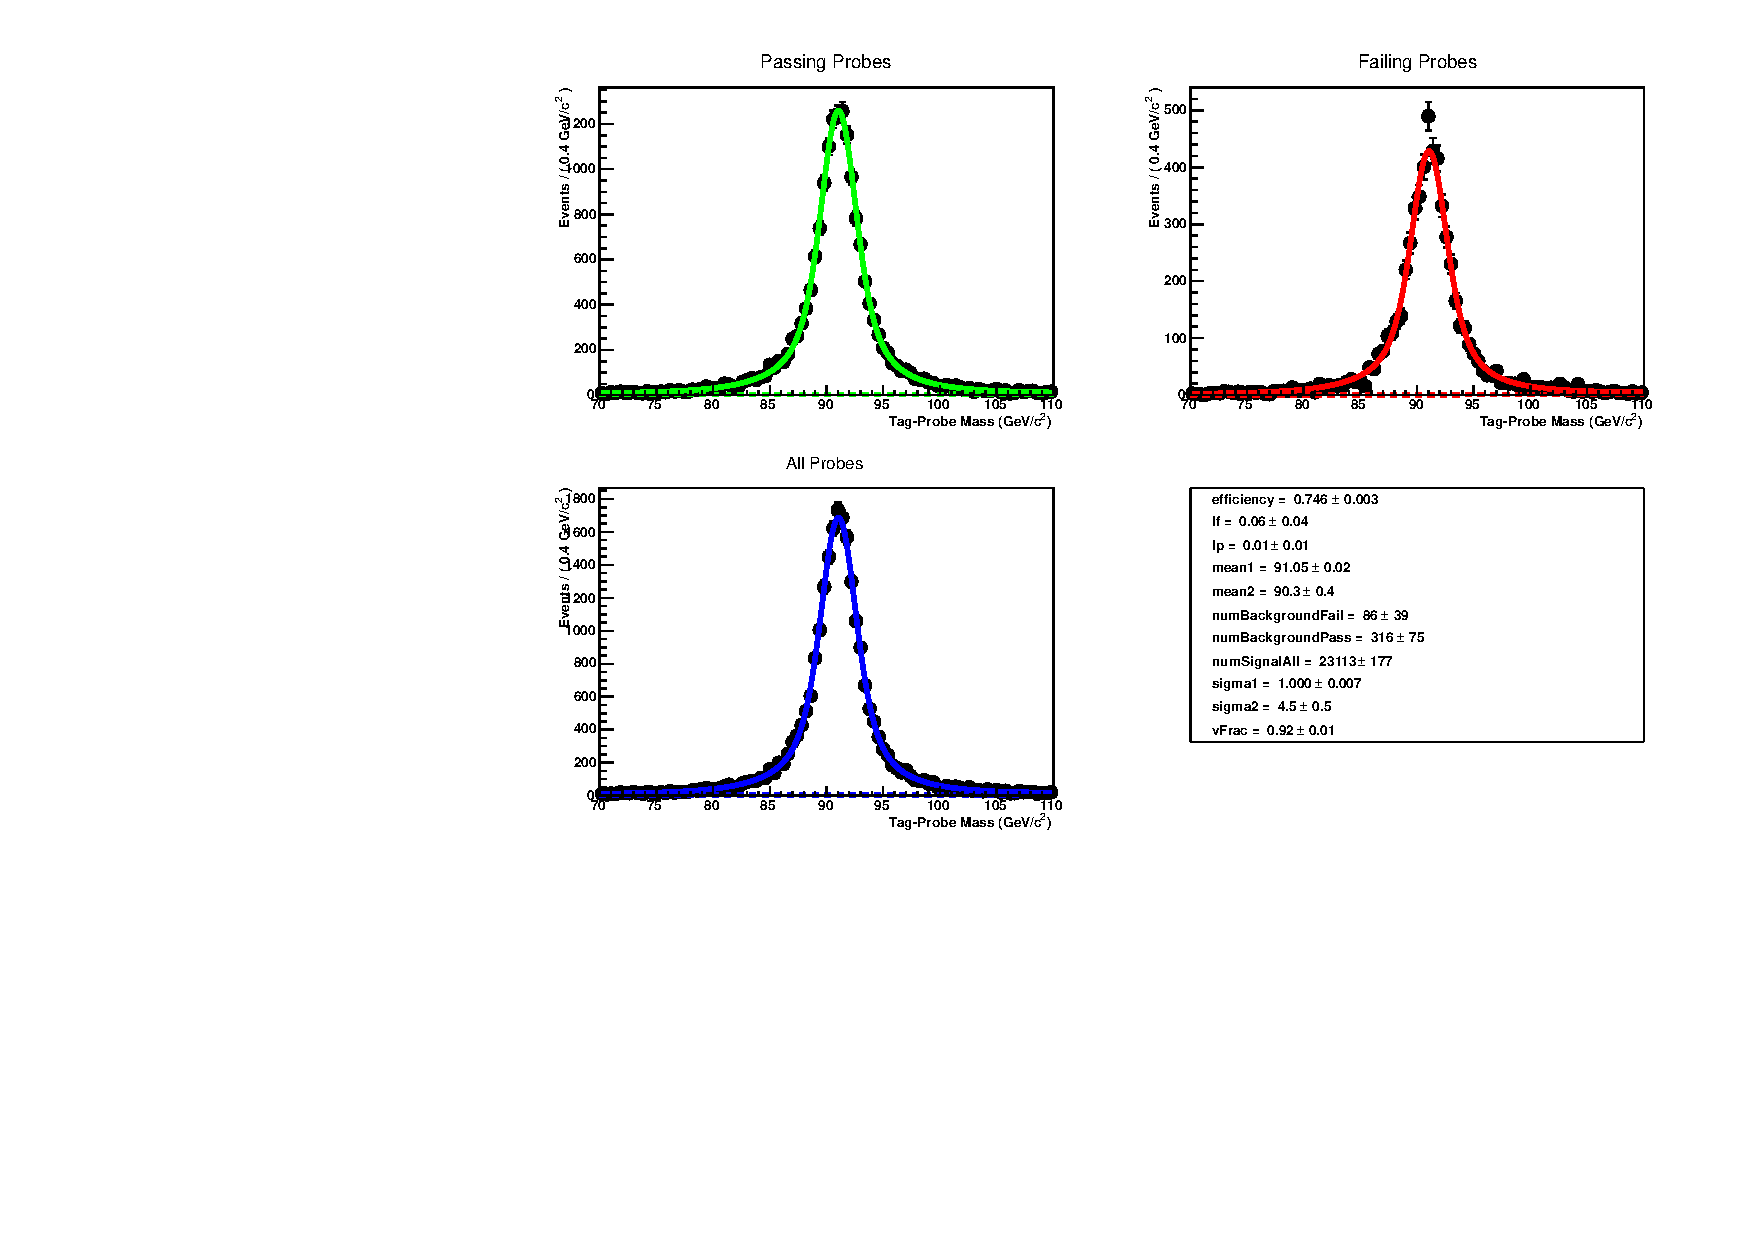
\includegraphics[width=0.95\textwidth]{figures/muonly/FitCanvasMCEtaBin6}
% \end{center}
% \caption[Example fits to invariant mass distributions
%in the tag-and-probe procedure for the \muononly\ analysis for MC.]
%{Same as Fig.~\ref{fig:MuOnlyTagProbeFitData} but for MC.}
%    \label{fig:MuOnlyTagProbeFitMC}
%\end{figure}

Figure~\ref{fig:MuOnlyTagProbeEff} shows the efficiency for the probes
to pass the preselection, except for the selection on $p_T$, against the probe
$p_T$, $\eta$, and the number of primary vertices in the event.
Overall the efficiency is approximately 75\% in data and 80\% in the MC sample.
The efficiency is mostly flat versus $p_T$ and number of vertices but does depend
on $\eta$.  The MC simulation is scaled by an $\eta$ dependent scale factor to correct for the discrepancy.

\begin{figure}
 \begin{center}
  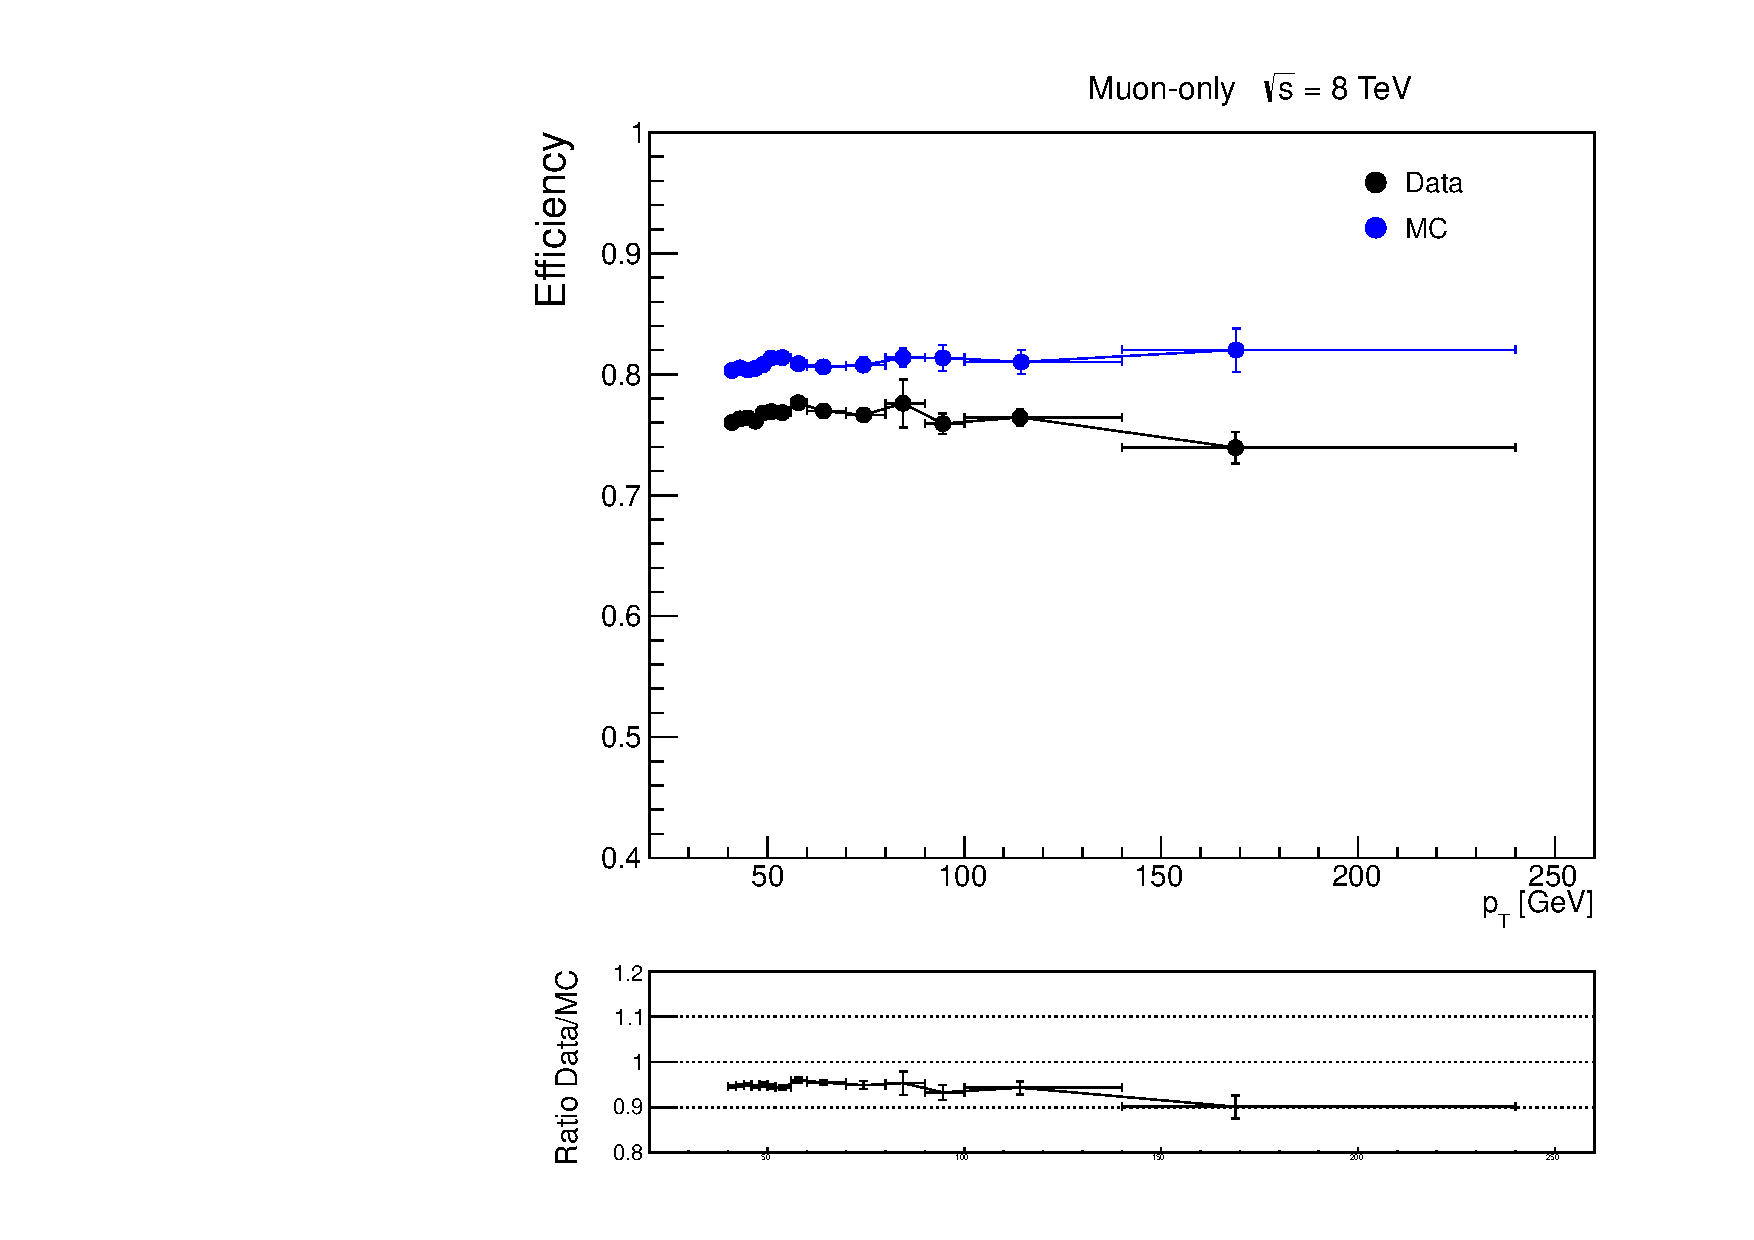
\includegraphics[clip=false, trim=0.0cm 0cm 0cm 0cm, width=0.44\textwidth]{figures/muonly/pteff_Comp}
  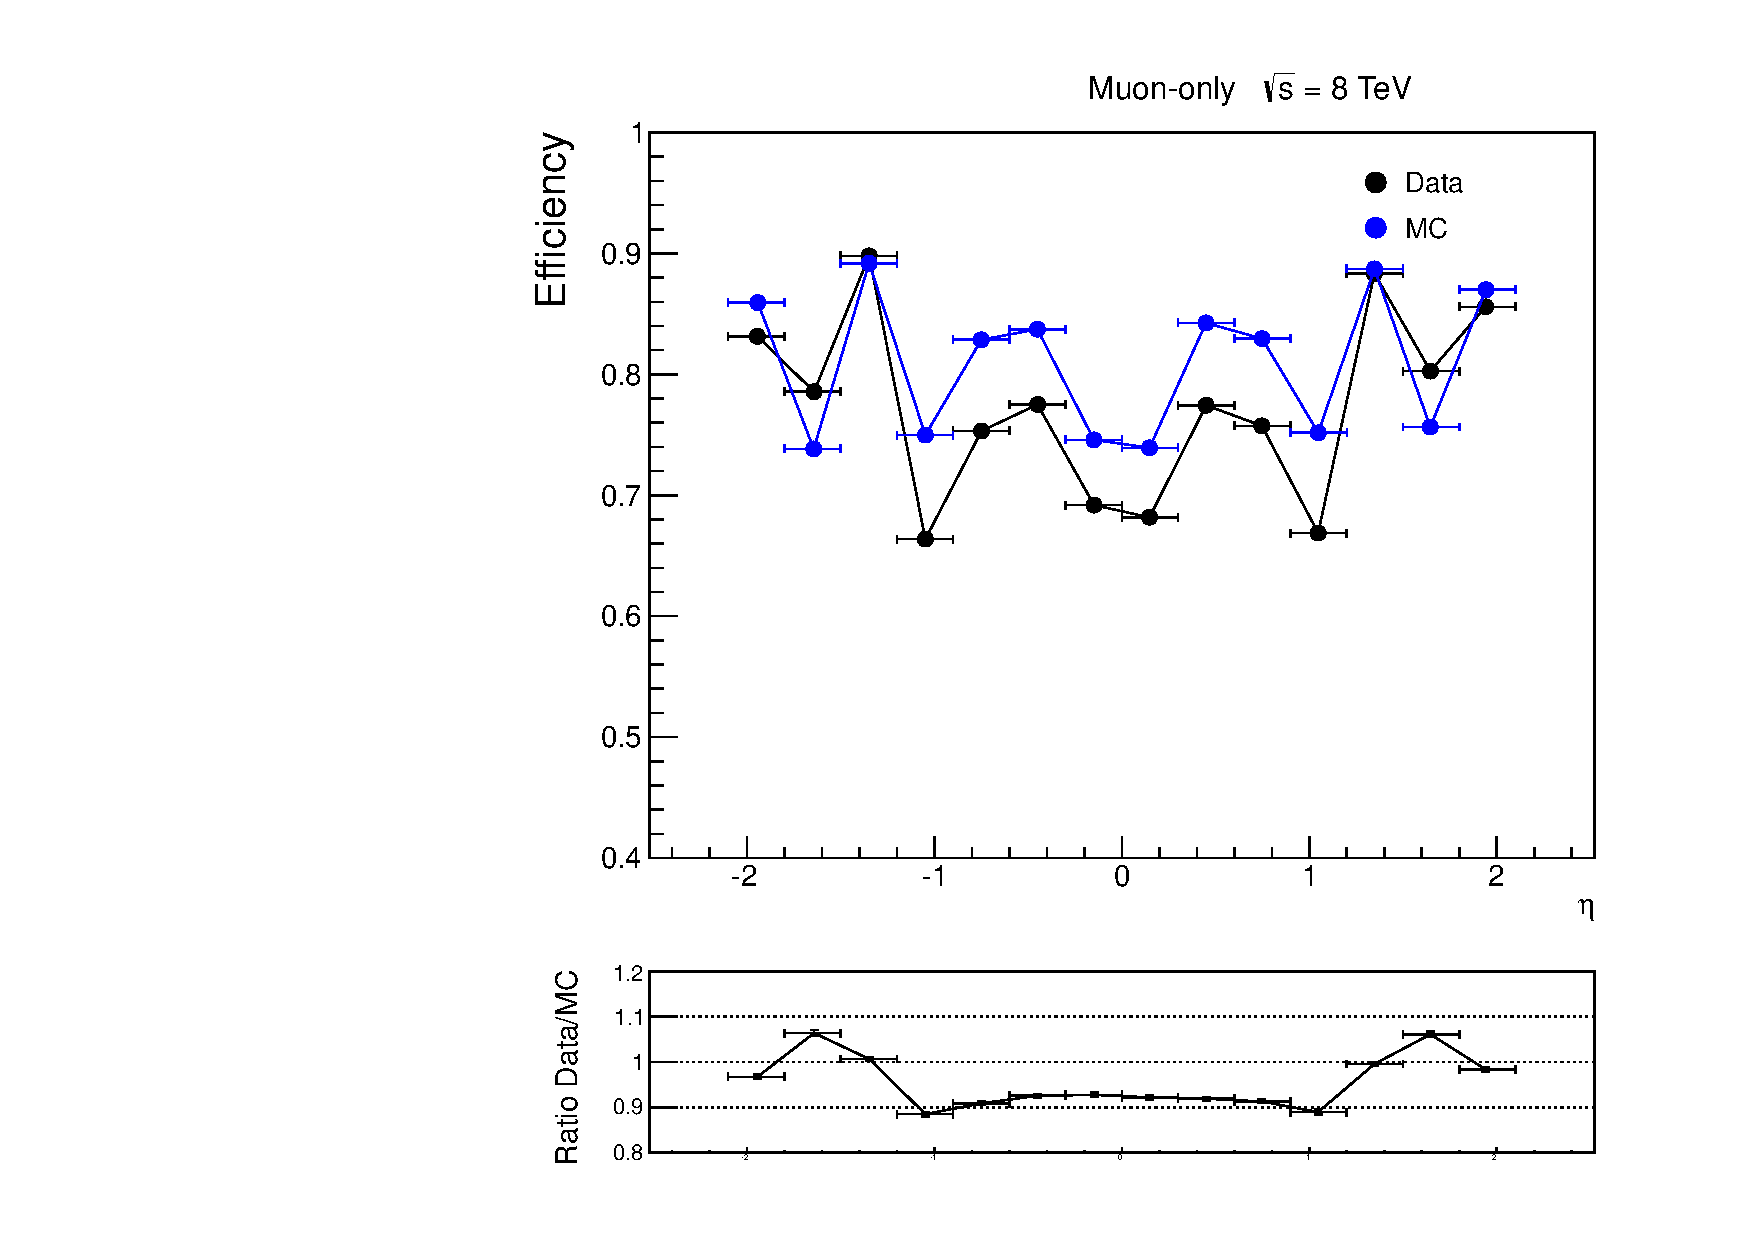
\includegraphics[clip=false, trim=0.0cm 0cm 0cm 0cm, width=0.44\textwidth]{figures/muonly/etaeff_Comp}
  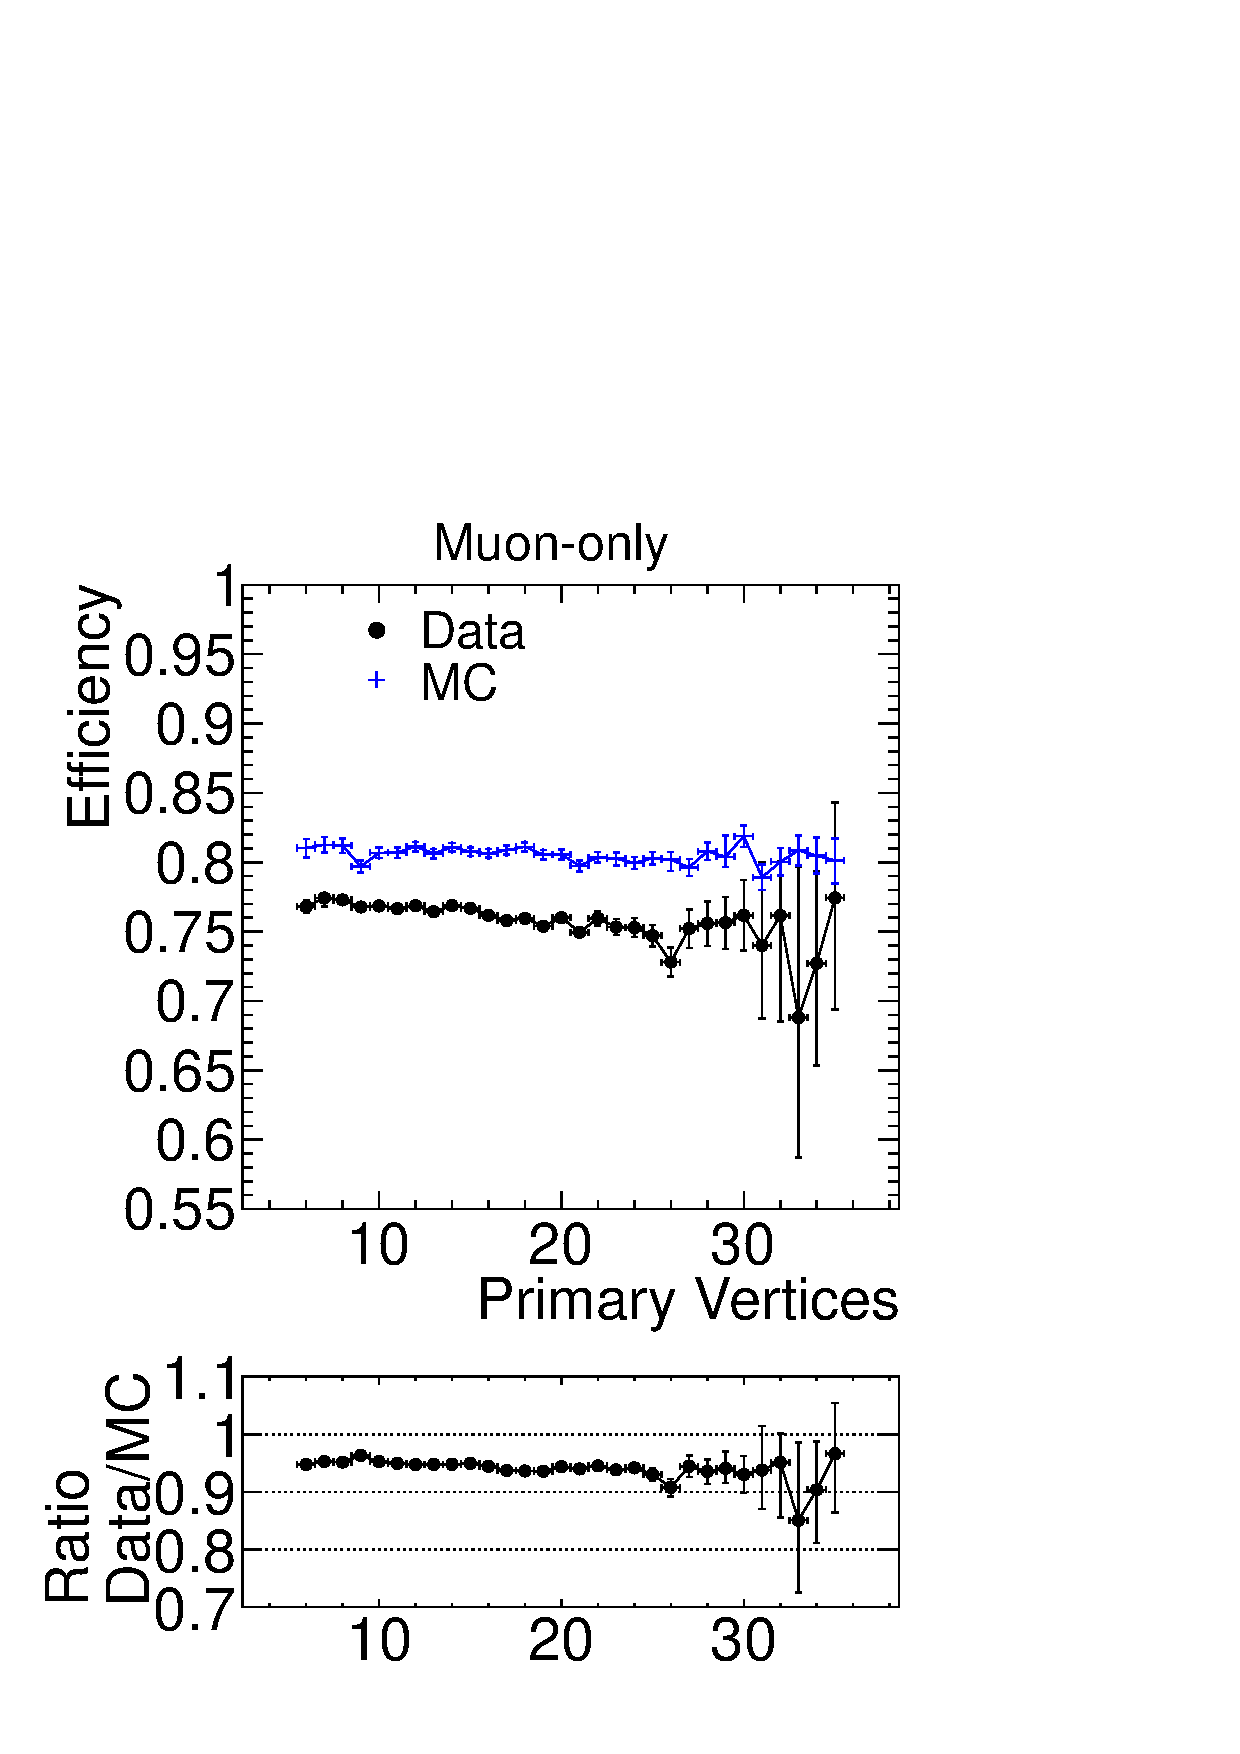
\includegraphics[clip=false, trim=0.0cm 0cm 0cm 0cm, width=0.44\textwidth]{figures/muonly/PVeff_Comp}
 \end{center}
 \caption[Efficiency to pass preselection cuts for the \muononly\ analysis as a function of \pt, $\eta$, and number of primary vertices]
{Efficiency to pass preselection cuts for the \muononly\ analysis.
Top row: As a function of $p_T$ (left) and $\eta$ (right)
Bottom row: As a function of number of primary vertices.}
   \label{fig:MuOnlyTagProbeEff}
\end{figure}